\documentclass[xcolor=dvipsnames,10pt]{beamer}
\mode<presentation>


\usepackage[active,tightpage]{preview}
%\setlength\PreviewBorder{5pt}%
%\usepackage[hidelinks]{hyperref}
%\usepackage{cite}
\usepackage{beamerthemesplit}
\usepackage{verbatim}
\usepackage[UKenglish]{babel}
\usepackage{listings}
\usepackage{latexsym}
\usepackage[utf8]{inputenc}
\usepackage{multirow}
\usepackage{listings}
\usepackage{color}
\usepackage{amsmath,amsthm,amssymb}
\usepackage[noend]{algpseudocode}
\usepackage[ruled,noline,linesnumbered]{algorithm2e}
\usepackage{pgf}
\usepackage{tikz}
\usetikzlibrary{automata,arrows,decorations.pathreplacing}
	\usetikzlibrary{positioning}
	\usetikzlibrary{backgrounds}
	\usetikzlibrary{arrows}
\usepackage{epstopdf}
\usepackage[caption=false]{subfig}

\usepackage{array}
\newcolumntype{C}[1]{>{\centering\arraybackslash}p{#1}}


%% style for drawing RNNs
\tikzstyle{RNN_style}=[
	->,shorten >=1pt,auto,node distance=1.5cm, thick,
	neuron/.style={circle,fill=white!50,node distance =1.2cm,draw,minimum 	size=0.7cm,font=\sffamily\normalsize},
	missing/.style={rectangle,node distance =1.2cm,draw=none,minimum size=0.7cm,font=\sffamily\Huge\bfseries},
	label/.style={node distance=1.2cm,rectangle,draw=none,minimum size=0.7cm,font=\sffamily\normalsize},
	layer/.style={rectangle,fill=white!50,draw,minimum width=4cm,font=\sffamily\normalsize},
	thick_edge/.style={line width=1pt},
	thin_edge/.style={line width=0.5pt}
]

%%Notation:

%%vectors
\renewcommand{\vec}[1]{\boldsymbol{#1}}
%%sets
\newcommand{\set}[1]{\mathcal{#1}}
%%matrixes
\newcommand{\mat}[1]{#1}
%%norm
\newcommand{\norm}[1]{\left\Vert #1 \right\Vert}
%%defeq
\newcommand{\defeq}{\triangleq}
%%
\newcommand{\net}[1]{\mathrm{#1}}
%% pair<x,y>
\newcommand{\pair}[2]{\langle#1,#2\rangle}


\graphicspath{ {./images/} }

%\usecolortheme[named=MidnightBlue]{structure}
%Warsaw Dresden Singapore Copenhagen Madrid AnnArbor
%\usetheme{Warsaw}
\usetheme{metropolis}
\setbeamercovered{transparent}
%\setbeamercolor{lowercolor}{fg=white , bg=MidnightBlue}
\setbeamertemplate{blocks}[rounded][shadow=true]
\setbeamertemplate{items}[default]
\setbeamertemplate{navigation symbols}{}

\title{Optimization methods for Recurrent Neural Networks training}
%\subtitle{A nice subtitle}
\date{20th April 2016}
\author{Giulio Galvan\\ Gsss }
\institute{Università degli studi di Firenze}
\titlegraphic{\hfill
\includegraphics[height=1.5cm]{stemma}}  % %TODO put the logo img here
\usetitlepagetemplate{
	\begin{center}
		%\pgfuseimage{salom}
		%\vskip0.5ex
		\begin{figure}
			
\includegraphics[width=3cm]{stemma.pdf}
		\end{figure}
		\vskip4ex
		\begin{beamerboxesrounded}[lower=lowercolor, shadow=true]{}
			\begin{center}
				\large{\textbf{Optimization methods for Recurrent Neural Networks training}}\\
				
			\end{center}
		\end{beamerboxesrounded}
		\vskip4ex
		\begin{footnotesize}
			\begin{center}
				Giulio Galvan
			\end{center}
			\begin{columns}
				\begin{column}{0.4\textwidth}
					\flushleft{\textbf{Relatori}: }\\
					Prof. Marco Sciandrone \\
					Prof. Luís  Nunes Vicente
				\end{column}
				\begin{column}{0.4\textwidth}
					\flushright{\textbf{Correlatore}: }\\
					Prof. Fabio Schoen
				\end{column}
			\end{columns}
			\vskip 1cm
			20th April 2016
		\end{footnotesize}
		
	\end{center}
}


\begin{document}
%\maketitle
\frame{\titlepage}
\section{Introduction}

\subsection{The model}
\begin{frame}{The model}
	
\begin{block}{Def: RNN}
	Given an input sequence $\{\vec{u}\}_{t=1,...,T}$, with $ \vec{u}_t \in \mathbb{R}^p$, the output sequence of a RNN $\{\vec{y}\}_{t=1,...,T}$, with $\vec{y}_t \in \mathbb{R}^o$,  is defined by the following:
\begin{align}
		&\vec{y}^t \defeq F(\vec{z}^t)\\
		&\vec{z}^t \defeq \mat{W}^{out}\cdot\vec{a}^t + \vec{b}^{out}\\
		&\vec{a}^t \defeq \mat{W}^{rec}\cdot\vec{h}^{t-1}+\mat{W}^{in}\cdot\vec{u}^t+\vec{b}^{rec}\\
		&\vec{h}^t \defeq  \sigma(\vec{a}^t) \\
		&\vec{h}^0 \defeq \overrightarrow{0},
\end{align}
where $\sigma(\cdot):\mathbb{R}\rightarrow\mathbb{R}$ is a non linear function applied element-wise called \textbf{activation function}, $F(\cdot)$ is called \textbf{output function}. 
\end{block}

\begin{block}{}
	The parameters of the net are $\{\mat{W}^{out}, \mat{W}^{in},  \mat{W}^{rec}, \vec{b}^{rec}, \vec{b}^{out}\}$.
\end{block}
\end{frame}

\begin{frame}
	\tikzstyle{rnn_style}=[->,shorten >=1pt,auto,node distance=1.5cm,
	thick,
	neuron/.style={circle,fill=white!50,node distance =1.2cm,draw,minimum size=0.7cm,font=\sffamily\Large\bfseries},
	missing/.style={rectangle,node distance =1.2cm,fill=white!50,draw=none,minimum size=0.7cm,font=\sffamily\Huge\bfseries},
	label/.style={node distance=1.2cm,rectangle,fill=white!50,draw=none,minimum size=0.7cm,font=\sffamily\normalsize},
	layer/.style={rectangle,fill=white!50,draw,minimum width=4cm,font=\sffamily\normalsize},
	loopStyle/.style={in=120,out=60, distance=2.5cm},]
	\begin{figure}[!h]
		\centering
		\resizebox{7cm}{!}{
		\begin{tikzpicture}[rnn_style]
		
		\node[neuron]    (x0)       {};
		\node[neuron]    (x1)[right of=x0]   {};
		\node[neuron]    (x2)[right of=x1]   {};
		\node[missing]   (x3)[right of=x2]   { $\hdots$};
		\node[neuron]    (xn)[right of=x3]   {};
		
		\node[label]    (u0)[below of=x0]   {$u_0[t]$};
		\node[label]    (u1)[below of=x1]   {$u_1[t]$};
		\node[label]    (u2)[below of=x2]   {$u_2[t]$};
		\node[label]    (un)[below of=xn]   {$u_n[t]$};
		
		
		\node[layer] (hl)[above of=x2,node distance=2cm] {Hidden layer};
		\node[neuron](b) [right of=hl,node distance=3cm] {};
		\node[label] (b_l) [right of=b] {bias=1};
		\node[layer] (ol)[above of=hl,node distance=2cm] {Output layer};
		
		\node[neuron] (o1) at (0,5.5) {};
		\node[neuron] (o2)[right of=o1] {};
		\node[neuron] (o3)[right of=o2] {};
		\node[missing](o4)[right of=o3] {$\hdots$};
		\node[neuron] (on)[right of=o4] {};
		
		
		\node[label]    (y0)[above of=o1]   {$y_0[t]$};
		\node[label]    (y1)[above of=o2]   {$y_1[t]$};
		\node[label]    (y2)[above of=o3]   {$y_2[t]$};
		\node[label]    (yn)[above of=on]   {$y_n[t]$};
		
		
		\path[->] (x0) edge [] node[]{$W_{in}$}   (hl)
		(x1) edge []   (hl)
		(x2) edge []   (hl)
		(xn) edge []   (hl)
		(u0) edge []   (x0)
		(u1) edge []   (x1)
		(u2) edge []   (x2)
		(un) edge []   (xn)
		(ol) edge []   (o1)
		(ol) edge []   (o2)
		(ol) edge []   (o3)
		(ol) edge []   (on)
		(o1) edge []   (y0)
		(o2) edge []   (y1)
		(o3) edge []   (y2)
		(on) edge []   (yn)
		(hl) edge []  node[]{$W_{out}$} (ol)
		(b)  edge [bend left,dotted,in= 160]  node[]{$b_{rec}$} (hl)
		(b)  edge [bend left,dotted,anchor=west, in= -160]  node[]{$b_{out}$} (ol)
		(hl) edge [loop ,in=-160,out=160, distance=3cm,anchor=east ]      node [align=center]  {$W_{rec} $} (hl);
		
		\end{tikzpicture}
		}
		\caption{$\net{RNN}$ model.}
		\label{rnn_model}
	\end{figure}
\end{frame}

\subsection{The optimization problem}
\begin{frame}{The optimization problem}
Given a dataset $D$:
\begin{equation}
D\defeq\{\{\overline{\vec{u}}^{(i)}\}_{t=1,...,T}, \overline{\vec{u}}^{(i)}_t \in \mathbb{R}^p, \{\overline{\vec{y}}^{(i)}\}_{t=1,...,T}, \overline{\vec{y}}^{(i)}_t \in \mathbb{R}^o;  i=1,...,N\}
\end{equation}
we define a loss function $L_D(\vec{x})$ over $D$  as
\begin{equation}
L_D(\vec{x})\defeq\frac{1}{N}\sum_{i=1}^N \sum_{t=1}^T L_t(\overline{\vec{y}}_t^{(i)},\vec{y}_t^{(i)}(\vec{x})),
\end{equation}
where $L_t(\cdot, \cdot)$ is an arbitrary loss function for the time step $t$ and $\vec{x}$ represents all the parameters of the network.
The problem is \begin{equation}
\min_{\vec{x}} L_D(\vec{x})
\end{equation}
\end{frame}

\begin{frame}{Some learning examples}

	\begin{itemize}
		\item Regression: mean squared error, linear output
		\begin{equation}
			L(\vec{y}, \vec{t}) = \frac{1}{M}\sum_{i=1}^M (y_i-t_i)^2, \quad F(\vec{y}) = \vec{y}.
		\end{equation}
		\item Binary classification: hinge loss, linear output
		\begin{equation}
			L(y, t) = \max(0,1-t\cdot y ), \quad F(y) = y.
		\end{equation}
		\item Multi-way classification: cross entropy loss, softmax output
		\begin{equation}
						L(\vec{y}, \vec{t}) = -\frac{1}{M}\sum_{i=1}^M \log(y_i)\cdot t_i, \quad F(y_j) = \frac{e^{y_j}}{\sum_{i=1}^M e^{y_i}}.
		\end{equation}
	\end{itemize}
\end{frame}

\begin{frame}{Stochastic gradient descent (SGD)}
\begin{algorithm}[H]
	\KwData{\\
		\Indp
		$D=\{\pair{\vec{u}^{(i)}}{\vec{y}^{(i)}}\}$: training set\\
		$\vec{x}_0$: candidate solution \\
		$m$: size of each mini-batch\\
	}
	
	\KwResult{\\
		\Indp $\vec{x}$: solution
	}
	\BlankLine
	
	$\vec{x} \gets \vec{x}_0$\\
	\While{stop criterion}{
		
		$I$ $\gets$ select $m$ training example $\in D$  \\
		$\alpha \gets$ compute learning rate \\
		$\vec{x} \gets \vec{x} - \alpha \sum_{ i\in I}\nabla_{\vec{x}} L(\vec{x}; \pair{\vec{u}^{(i)}}{\vec{y}^{(i)}})$\\
	}
	\caption{Stochastic gradient descent}
	\label{algo:sgd}
\end{algorithm}	
\end{frame}
\begin{frame}{}
	\begin{itemize}
		\item Nemirovski (2009)\cite{Nemirovski}: proof of convergence in the convex case
		\item there are no theoretical guarantees in the non-convex case 
		\item in practice it always works: SGD is the standard framework in most of neural networks applications.
	\end{itemize}
\end{frame}
\section{Gradient of a RNN}


%\begin{frame}
%	
%	Let's consider a single output unit $u$, and a weight $w_{lj}$, we have
%	
%	\begin{align}
%	\label{sum_over_time}
%	\frac{\partial a^t_u}{\partial w_{lj}} &= \sum_{k=1}^t \frac{\partial a_u^t}{\partial a^k_l} \cdot \frac{\partial a^k_l}{\partial w_{lj}}\\
%	&= \sum_{k=1}^t \delta^{tk}_{lu} \cdot \phi_j^{t-1}
%	\end{align}
%	where
%	\begin{equation}
%	\delta_{lu}^{tk} \triangleq \frac{\partial a_u^t}{\partial a^k_l}.
%	\end{equation}
%	
%	Let $P(l)$ be the set of parents of neuron $l$, defined as the set of parents in the unfolded network.
%	
%	\begin{equation}
%	\delta_{lu}^{tk} = \sum_{h\in P(l)} \delta_{hu}^{tk} \cdot \sigma'(a_h^{t-1})\cdot w_{hl}
%	\end{equation}
%\end{frame}
%\begin{frame}
%	\begin{figure}
%		\centering
%		\resizebox{5cm}{!}{
%		\begin{tikzpicture}[RNN_style]
%		
%		
%		\node[neuron]    (x1)[]   {$u$};
%		\node[neuron]    (x2)[right of=x1]   {$l$};
%		\node[neuron]    (x3)[right of=x2]   {};
%		\node[label]     (xl)[left of=x1] {$t$};
%		
%		\node[neuron]    (h1)[below of =x1]   {$u$};
%		\node[neuron]    (h2)[right of=h1]   {$l$};
%		\node[neuron]    (h3)[right of=h2]   {};
%		\node[label]     (hl)[left of=h1] {$\hdots$};
%		
%		\node[neuron]    (y1)[below of=h1]   {$u$};
%		\node[neuron]    (y2)[right of=y1]   {$l$};
%		\node[neuron]    (y3)[right of=y2]   {};
%		\node[label]     (yl)[left of=y1] {$k+2$};
%		
%		
%		\node[neuron]    (z1)[below of=y1]   {$u$};
%		\node[neuron]    (z2)[right of=z1]   {$l$};
%		\node[neuron]    (z3)[right of=z2]   {};
%		\node[label]     (zl)[left of=z1] {$k+1$};
%		
%		\node[neuron]    (w1)[below of=z1]   {$u$};
%		\node[neuron]    (w2)[right of=w1]   {$l$};
%		\node[neuron]    (w3)[right of=w2]   {};
%		\node[label]     (wl)[left of=w1] {$k$};
%		
%		
%		%   \node[label]      (lu)[left of=u] {$u$};
%		%   \node[label]      (ll)[left of=z1] {$l$};
%		
%		
%		\path[->] (h1) edge [thick_edge]  (x1)
%		(h1) edge [thin_edge]   (x2)
%		(h1) edge [thin_edge]   (x3)
%		(h2) edge [thick_edge]  (x1)
%		(h2) edge [thin_edge]   (x2)
%		(h2) edge [thin_edge]   (x3)
%		(h3) edge [thick_edge]  (x1)
%		(h3) edge [thin_edge]   (x2)
%		(h3) edge [thin_edge]   (x3);
%		
%		\path[->] (y1) edge [thick_edge]   (h1)
%		(y1) edge [thick_edge]   (h2)
%		(y1) edge [thick_edge]   (h3)
%		(y2) edge [thick_edge]   (h1)
%		(y2) edge [thick_edge]   (h2)
%		(y2) edge [thick_edge]   (h3)
%		(y3) edge [thick_edge]   (h1)
%		(y3) edge [thick_edge]   (h2)
%		(y3) edge [thick_edge]   (h3);
%		
%		
%		\path[->] (z1) edge [thin_edge]   (y1)
%		(z1) edge [thick_edge]  (y2)
%		(z1) edge [thin_edge]   (y3)
%		(z2) edge [thick_edge]  (y1)
%		(z2) edge [thick_edge]  (y2)
%		(z2) edge [thick_edge]  (y3)
%		(z3) edge [thin_edge]   (y1)
%		(z3) edge [thin_edge]   (y2)
%		(z3) edge [thin_edge]   (y3);
%		
%		\path[->] (w1) edge [thin_edge]   (z1)
%		(w1) edge [thick_edge]  (z2)
%		(w1) edge [thin_edge]   (z3)
%		(w2) edge [thin_edge]   (z1)
%		(w2) edge [thin_edge]   (z2)
%		(w2) edge [thin_edge]   (z3)
%		(w3) edge [thin_edge]   (z1)
%		(w3) edge [thin_edge]   (z2)
%		(w3) edge [thin_edge]   (z3);
%		
%		
%		\end{tikzpicture}
%		}
%		\caption{Nodes involved in $\frac{\partial a^t_u }{\partial a^k_l}$.}
%		\label{deriv_arcs_rnn}
%	\end{figure}
%\end{frame}


\begin{frame}{Gradient structure: unfolding}
	
	\begin{figure}[h!]
		\centering
		\resizebox{8cm}{!}{
			\begin{tikzpicture}[RNN_style, loopStyle/.style={in=120,out=60, distance=2.5cm}]
			
			%t=0
			\node[layer] (hl1) {Hidden layer t=0};
			
			\node[neuron]    (x0)[below left=0.3cm and 1cm of hl1]       {};
			\node[label]    (u0)[left of=x0]   {$\vec{u}^1$};
			
			
			
			\node[neuron] (o0) [above right=0.3cm and 1cm of hl1] {};
			\node[label]    (y0)[right of=o0]   {$\vec{y}^1$};
			
			%t=1
			\node[layer] (hl2)[above of=hl1,node distance=2.5cm] {Hidden layer t=1};
			
			\node[neuron]    (x1)[below left=0.3cm and 1cm of hl2]      {};
			\node[label]    (u1)[left of=x1]   {$\vec{u}^2$};
			
			
			\node[neuron] (o1) [above right=0.3cm and 1cm of hl2] {};
			\node[label]    (y1)[right of=o1]   {$\vec{y}^2$};
			
			%dots
			\node[label,font=\sffamily\Huge\bfseries] (hld)[above of=hl2,node distance=2cm] {$\hdots$};
			
			%t=T
			\node[layer] (hlT)[above of=hld,node distance=2cm] {Hidden layer t=T};
			
			\node[neuron]    (xT)[below left=0.3cm and 1cm of hlT]      {};
			\node[label]    (uT)[left of=xT]   {$\vec{u}^T$};
			
			
			\node[neuron] (oT) [above right=0.3cm and 1cm of  hlT] {};
			\node[label]    (yT)[right of=oT]   {$\vec{y}^T$};
			
			
			%biases
			\node[neuron](b) [right of=y1,node distance=1.4cm] {};
			\node[label] (b_l) [above of=b,node distance=0.7cm] {bias=1};
			
			
			\path[->] (x0) edge [bend right] node[]{$W^{in}$}   (hl1)
			(u0) edge []   (x0)
			(o0) edge []   (y0)
			(x1) edge [bend right] node[]{$W^{in}$} (hl2)
			(u1) edge []   (x1)
			(o1) edge []   (y1)
			(xT) edge [bend right] node[]{$W^{in}$} (hlT)
			(uT) edge []   (xT)
			(oT) edge []   (yT)
			
			
			(hl1) edge [bend left]  node[]{$W^{out}$} (o0)
			(hl2) edge [bend left]  node[]{$W^{out}$} (o1)
			(hlT) edge [bend left]  node[]{$W^{out}$} (oT)
			
			(b)  edge [bend left,dotted,in = 90]  node[]{$b^{out}$} (o0)
			(b)  edge [bend left, dotted, in = 90,out=80]  node[]{$b^{rec}$} (hl1)
			(b)  edge [bend left, dotted]  node[]{$b^{rec}$} (hl2)
			(b)  edge [bend left,dotted]  node[]{$b^{out}$} (o1)
			(b)  edge [bend left, dotted,in = 200]  node[]{$b^{rec}$} (hlT)
			(b)  edge [bend left,dotted,in =200]  node[]{$b^{out}$} (oT)
			(hl1) edge [] node[]{$W^{rec} $} (hl2)
			(hl2) edge [] node[]{$W^{rec} $} (hld)
			(hld) edge [] node[]{$W^{rec} $} (hlT);
			
			\end{tikzpicture}
		}
%		\caption{Unfolding of a $\net{RNN}$}
		\label{rnn_unfolding}
	\end{figure}
\end{frame}

\begin{frame}{Gradient structure: calculus}
	Consider, for ease of notation, the case where the loss function $L(\bar{\vec{u}}, \bar{\vec{y}})$ is defined only on the last step $\tau$. Let $g(\vec{x}): \mathbb{R}$ be the function defined by
	$$g(\vec{x}) \triangleq L(F(\vec{z}^\tau(\vec{\bar{\vec{u}};x}),\bar{\vec{y}}_\tau )).$$
	
	We compute the gradient as:
	\begin{align}
	\frac{\partial g}{\partial \mat{W}^{rec}} 
	&= \frac{\partial g}{\partial \vec{a}^\tau} \cdot \frac{\partial \vec{a}^\tau}{\partial \mat{W^{rec}}}\\
	&=  \nabla L^T \cdot J(F) \cdot \frac{\partial \vec{z}^\tau}{\partial \vec{a}^\tau} \cdot \frac{\partial \vec{a}^\tau}{\partial \mat{W}^{rec}}.
	\end{align}
\end{frame}

\begin{frame}
	In matrix notation we have:
	
	\begin{equation}
	\frac{\partial \vec{a}^t}{\partial \mat{W}^{rec}} = \sum_{k=1}^t \frac{\partial \vec{a}^t}{\partial \vec{a}^k} \cdot \frac{\partial^+ \vec{a}^k}{\partial \mat{W}^{rec}}
	\end{equation}
	
	
	\begin{equation}
	\frac{\partial^+ a^{k}}{\partial \mat{W}_j^{rec}} =
	\begin{bmatrix}
	h_j^{k}    & 0                & \cdots      & \cdots       & 0  \\
	0               & h_j^{k}     & \cdots      & \cdots       & 0  \\
	\vdots          & \vdots           & \ddots      & \vdots       &\vdots\\
	0               & \cdots           & \cdots      & \cdots       & h^{k}_{j}
	\end{bmatrix}
	\end{equation}
	
	\begin{align}
	\frac{\partial \vec{a}^t}{\partial \vec{a}^k} &= \frac{\partial \vec{a}^t}{\partial \vec{a}^{k+1}} \cdot diag(\sigma'(\vec{a}^k)) \cdot \mat{W}^{rec} \\
	&= \prod_{i=t-1}^{k} diag(\sigma'(\vec{a}^i)) \cdot \mat{W}^{rec}
	\label{rnn_delta}.
	\end{align}
	
	The derivatives with respect to the other variables are computed in a similar fashion.
	
	
\end{frame}

\begin{frame}{Gradient structure: temporal components}
	
	Putting all together we obtain:
	\begin{align}
	\nabla_{\mat{W^{rec}}} g  &= \sum_{k=1}^{\tau} \frac{\partial g}{\partial \vec{a}^{\tau}} \cdot \frac{\partial \vec{a}^{\tau}}{\partial \vec{a}^k} \cdot \frac{\partial^+ \vec{a}^k}{\partial \mat{W}^{rec}}\\
	&\defeq \sum_{k=1}^{\tau} \nabla_{\mat{W^{rec}}} L_{|k}.
	\end{align}
	
	We refer to $\nabla_{\vec{x}} g_{|k}$ as the \textbf{temporal gradient} for time step $k$ w.r.t. the variable $\vec{x}$, and it is easy to see that it is the gradient we would compute if we replicated the variable $\vec{x}$ for each time step and took the derivatives w.r.t. to its k-th replicate.
\end{frame}
\section{The vanishing gradient problem}
\subsection{The addition task}
\begin{frame}{A pathological problem example}


An input sequence:

\vspace{1em}

\begin{tabular}{|c|c|c|c|c|c|c|c|c|c}
	\hline  marker & 0&  1&  0&  $\hdots$& 0 & 1 & 0 & 0  \\ 
	  value & 0.3&  \textbf{0.7}&  0.1&  $\hdots$& 0.2& \textbf{0.4} & 0.6& 0.9  \\ 
	\hline 
\end{tabular}

\vspace{1em}
The predicted output should be the sum of the two one-marked positions (1.1). 
\pause
\vspace{1em}
\begin{block}{Why is this a difficult problem?}
	Because of its long time dependencies.
\end{block}

\end{frame}
\subsection{Gradient calculus}
\begin{frame}{Gradient}
	Let $L_t(\bar{\vec{u}}, \bar{\vec{y}})$ the loss function for the time step $t$ and  $g_t(\vec{x}): \mathbb{R}$ be the function defined by
	$$g_t(\vec{x}) \triangleq L_t(F(\vec{z}^t(\vec{\bar{\vec{u}};x}),\bar{\vec{y}}_t ))$$
	and $$g(\vec{x}) \triangleq \sum_{t=1}^T g_t(\vec{x})$$
	
	
	\begin{align}
	\frac{\partial g}{\partial \mat{W}^{rec}} &= \sum_{t=1}^T \nabla L_t^T \cdot J(F) \cdot \frac{\partial \vec{z}^t}{\partial \vec{a}^t} \cdot \frac{\partial \vec{a}^t}{\partial \mat{W}^{rec}}\\
	&= \sum_{t=1}^T\frac{\partial g_t}{\partial \vec{a}^t} \cdot \frac{\partial \vec{a}^t}{\partial \mat{W^{rec}}}
	\end{align}
\end{frame}
\begin{frame}
	
	Let's consider a single output unit $u$, and a weight $w_{lj}$, we have
	
	\begin{align}
	\label{sum_over_time}
	\frac{\partial a^t_u}{\partial w_{lj}} &= \sum_{k=1}^t \frac{\partial a_u^t}{\partial a^k_l} \cdot \frac{\partial a^k_l}{\partial w_{lj}}\\
	&= \sum_{k=1}^t \delta^{tk}_{lu} \cdot \phi_j^{t-1}
	\end{align}
	where
	\begin{equation}
	\delta_{lu}^{tk} \triangleq \frac{\partial a_u^t}{\partial a^k_l}.
	\end{equation}
	
	Let $P(l)$ be the set of parents of neuron $l$, defined as the set of parents in the unfolded network.
	
	\begin{equation}
	\delta_{lu}^{tk} = \sum_{h\in P(l)} \delta_{hu}^{tk} \cdot \sigma'(a_h^{t-1})\cdot w_{hl}
	\end{equation}
\end{frame}
\begin{frame}
	
	
	\begin{figure}
		\centering
		\resizebox{5cm}{!}{
		\begin{tikzpicture}[RNN_style]
		
		
		\node[neuron]    (x1)[]   {$u$};
		\node[neuron]    (x2)[right of=x1]   {$l$};
		\node[neuron]    (x3)[right of=x2]   {};
		\node[label]     (xl)[left of=x1] {$t$};
		
		\node[neuron]    (h1)[below of =x1]   {$u$};
		\node[neuron]    (h2)[right of=h1]   {$l$};
		\node[neuron]    (h3)[right of=h2]   {};
		\node[label]     (hl)[left of=h1] {$\hdots$};
		
		\node[neuron]    (y1)[below of=h1]   {$u$};
		\node[neuron]    (y2)[right of=y1]   {$l$};
		\node[neuron]    (y3)[right of=y2]   {};
		\node[label]     (yl)[left of=y1] {$k+2$};
		
		
		\node[neuron]    (z1)[below of=y1]   {$u$};
		\node[neuron]    (z2)[right of=z1]   {$l$};
		\node[neuron]    (z3)[right of=z2]   {};
		\node[label]     (zl)[left of=z1] {$k+1$};
		
		\node[neuron]    (w1)[below of=z1]   {$u$};
		\node[neuron]    (w2)[right of=w1]   {$l$};
		\node[neuron]    (w3)[right of=w2]   {};
		\node[label]     (wl)[left of=w1] {$k$};
		
		
		%   \node[label]      (lu)[left of=u] {$u$};
		%   \node[label]      (ll)[left of=z1] {$l$};
		
		
		\path[->] (h1) edge [thick_edge]  (x1)
		(h1) edge [thin_edge]   (x2)
		(h1) edge [thin_edge]   (x3)
		(h2) edge [thick_edge]  (x1)
		(h2) edge [thin_edge]   (x2)
		(h2) edge [thin_edge]   (x3)
		(h3) edge [thick_edge]  (x1)
		(h3) edge [thin_edge]   (x2)
		(h3) edge [thin_edge]   (x3);
		
		\path[->] (y1) edge [thick_edge]   (h1)
		(y1) edge [thick_edge]   (h2)
		(y1) edge [thick_edge]   (h3)
		(y2) edge [thick_edge]   (h1)
		(y2) edge [thick_edge]   (h2)
		(y2) edge [thick_edge]   (h3)
		(y3) edge [thick_edge]   (h1)
		(y3) edge [thick_edge]   (h2)
		(y3) edge [thick_edge]   (h3);
		
		
		\path[->] (z1) edge [thin_edge]   (y1)
		(z1) edge [thick_edge]  (y2)
		(z1) edge [thin_edge]   (y3)
		(z2) edge [thick_edge]  (y1)
		(z2) edge [thick_edge]  (y2)
		(z2) edge [thick_edge]  (y3)
		(z3) edge [thin_edge]   (y1)
		(z3) edge [thin_edge]   (y2)
		(z3) edge [thin_edge]   (y3);
		
		\path[->] (w1) edge [thin_edge]   (z1)
		(w1) edge [thick_edge]  (z2)
		(w1) edge [thin_edge]   (z3)
		(w2) edge [thin_edge]   (z1)
		(w2) edge [thin_edge]   (z2)
		(w2) edge [thin_edge]   (z3)
		(w3) edge [thin_edge]   (z1)
		(w3) edge [thin_edge]   (z2)
		(w3) edge [thin_edge]   (z3);
		
		
		\end{tikzpicture}
		}
		\caption{Nodes involved in $\frac{\partial a^t_u }{\partial a^k_l}$.}
		\label{deriv_arcs_rnn}
	\end{figure}
\end{frame}
\begin{frame}
	In matrix notation we have:
	
	\begin{equation}
	\frac{\partial \vec{a}^t}{\partial \mat{W}^{rec}} = \sum_{k=1}^t \frac{\partial \vec{a}^t}{\partial \vec{a}^k} \cdot \frac{\partial^+ \vec{a}^k}{\partial \mat{W}^{rec}}
	\end{equation}
	
	
	\begin{equation}
	\frac{\partial^+ a^{k}}{\partial \mat{W}_j^{rec}} =
	\begin{bmatrix}
	\phi_j^{k}    & 0                & \cdots      & \cdots       & 0  \\
	0               & \phi_j^{k}     & \cdots      & \cdots       & 0  \\
	\vdots          & \vdots           & \ddots      & \vdots       &\vdots\\
	0               & \cdots           & \cdots      & \cdots       & \phi^{k}_{j}
	\end{bmatrix}
	\end{equation}
	
	\begin{align}
	\frac{\partial \vec{a}^t}{\partial \vec{a}^k} &= \frac{\partial \vec{a}^t}{\partial \vec{a}^{k+1}} \cdot diag(\sigma'(\vec{a}^k)) \cdot \mat{W}^{rec} \\
	&= \prod_{i=t-1}^{k} diag(\sigma'(\vec{a}^i)) \cdot \mat{W}^{rec}
	\label{rnn_delta}.
	\end{align}
	
	The derivatives with respect to the other variables are computed in a similar fashion.

	
\end{frame}

\subsection{A sufficient condition}
\begin{frame}{Vanishing gradient: a sufficient condition}
	\begin{equation}
	\frac{\partial \vec{a}^t}{\partial \vec{a}^k} = \prod_{i=t-1}^{k}  diag(\sigma'(\vec{a}^i)) \cdot \mat{W}^{rec}.
	\label{eq:temporalComponent}
	\end{equation}
	
	Taking the singular value decomposition of $\mat{W}^{rec}$:
	\begin{equation}
	\mat{W}^{rec} =  \mat{S}\cdot\mat{D}\cdot\mat{V}^T
	\end{equation}
	where $\mat{S},\mat{V}^T$ are squared orthogonal matrices and $\mat{D}\defeq diag(\mu_1, \mu_2,...,\mu_r)$ is the diagonal matrix containing the singular values of $\mat{W}^{rec}$.
	Hence:
	\begin{equation}
	\frac{\partial \vec{a}^t}{\partial \vec{a}^k} = \prod_{i=t-1}^{k}  diag(\sigma'(\vec{a}^i)) \cdot \mat{S}\cdot \mat{D} \cdot \mat{V}^T
	\end{equation}
\end{frame}
\begin{frame}
	Since $\mat{U}$ and $\mat{V}$ are orthogonal matrix, hence $$\norm{\mat{U}}_2=\norm{\mat{V}^T}_2 = 1,$$ and $$\norm{diag(\lambda_1, \lambda_2,...,\lambda_r)}_2 = \lambda_{max},$$ we get
	\begin{align}
	\norm{\frac{\partial \vec{a}^t}{\partial \vec{a}^k}}_2 &= \norm{ (\prod_{i=t-1}^{k} diag(\sigma'(\vec{a}^i)) \cdot \mat{S}\cdot \mat{D} \cdot \mat{V}^T)}_2\\
	&\leq (\sigma'_{max} \cdot \mu_{max})^{t-k-1}
	\end{align}
\end{frame}


%\section{Existing solutions}
%The entirety of our work is based on the SGD framework described in section \ref{sec:sgd}. In particular we insisted on three phases of the algorithm, namely the initialization, the choice of the descent direction and the step size. We show that the initialization play a crucial role in the learning process and can, alone, dictate if the learning process will be "successful"\footnote{Here we refer to artificial task where a criterion for success is easily defined.} or not. We than propose a strategy to choose a descent direction which helps to deal with the vanishing gradient. As for the learning rate we use a technique which is entirely equivalent to the gradient clipping trick proposed in \cite{understandingExplodingGradients} which helps dealing with exploding gradients.


\section{Notation}
Before focusing on each phase we will introduce some notation which we will need in the following sections.

Consider a loss function $g$ for some time step $\tau$. Defining 
\begin{equation}
\nabla_{\mat{W_{rec}}} g_{|k}  \defeq \frac{\partial g}{\partial \vec{a}^{\tau}} \cdot \frac{\partial \vec{a}^{\tau}}{\partial \vec{a}^k} \cdot \frac{\partial^+ \vec{a}^k}{\partial \mat{W}^{rec}},
\end{equation}
and recalling the results of section \ref{sec:rnn_grad} we have
\begin{equation}
	\frac{\partial g_{\tau}}{\partial \mat{W}^{rec}} = \sum_{k=1}^{\tau} \nabla_{\mat{W_{rec}}} g_{|k}.
\end{equation}
We refer to $\nabla_{\vec{x}} g_{|k}$ as temporal gradient for time step $k$ w.r.t. the variable $\vec{x}$ and is easy to see that it is the gradient computed imagining to replicate variable $\vec{x}$ for each time step and taking the derivatives w.r.t. the variable for the step $k$.

The \textbf{vanishing gradient} problem appears then, under this new notation, when the norm of the temporal components $\nabla_{\vec{x}} g_{|k}$ are exponentially bigger for more recent time steps.

\section{Initialization}
The first moment of the learning process is the initialization of the variables. We found that the choice of the initial value for the recurrent matrix $\mat{W_{rec}}$ has a big impact on the entire learning process. Recall the results from section  \ref{sec:vanishing} where we saw that having such matrix too small singular values, more precisely $\sigma'_{max} \cdot \mu_{max} <1 $, is a sufficient condition for the gradient to vanish. Although a sufficient condition that, conversely, guarantees the gradient not to vanish is not known, the bounds on the singular values encourage to explore initialization techniques which produce matrices with higher singular values or more in general spectral radius. A similar suggestion, motivated by other consideration was given in the ESN field \cite{reservoirSummary}.

We propose an initialization scheme where the recurrent matrix is firstly sampled from some distribution\footnote{In all the experiments we always sample from a zero mean gaussian, but others distribution can be used as well.} and scaled to have a specified spectral radius as shown in \ref{algo:init_scaling}.

\begin{algorithm}[!h]
	\KwData{\\
		\Indp
		$\rho = $ desired spectral radius
	}
	\BlankLine

	$\mat{W_{rec}} \sim \mathcal{N}(0, \sigma^2)$\\
	$r \gets \mbox{spectral\_radius}(\mat{W_{rec}})$\\
	$\mat{W_{rec}}\gets \frac{\rho}{r} \cdot \mat{W_{rec}}$\\
	\KwRet{$\mat{W_{rec}}$}
	\caption{Recurrent weight matrix initialization scheme}
	\label{algo:init_scaling}
\end{algorithm}

 In figure \ref{fig:temporal_norms} we show, as an example, the temporal components w.r.t. all the variables of the model varying the spectral radius in [0.8, 0.9, 1, 1.1, 1.2] computed on a hundred samples for the temporal order task (INTRODUCE TASK).

\begin{figure}
    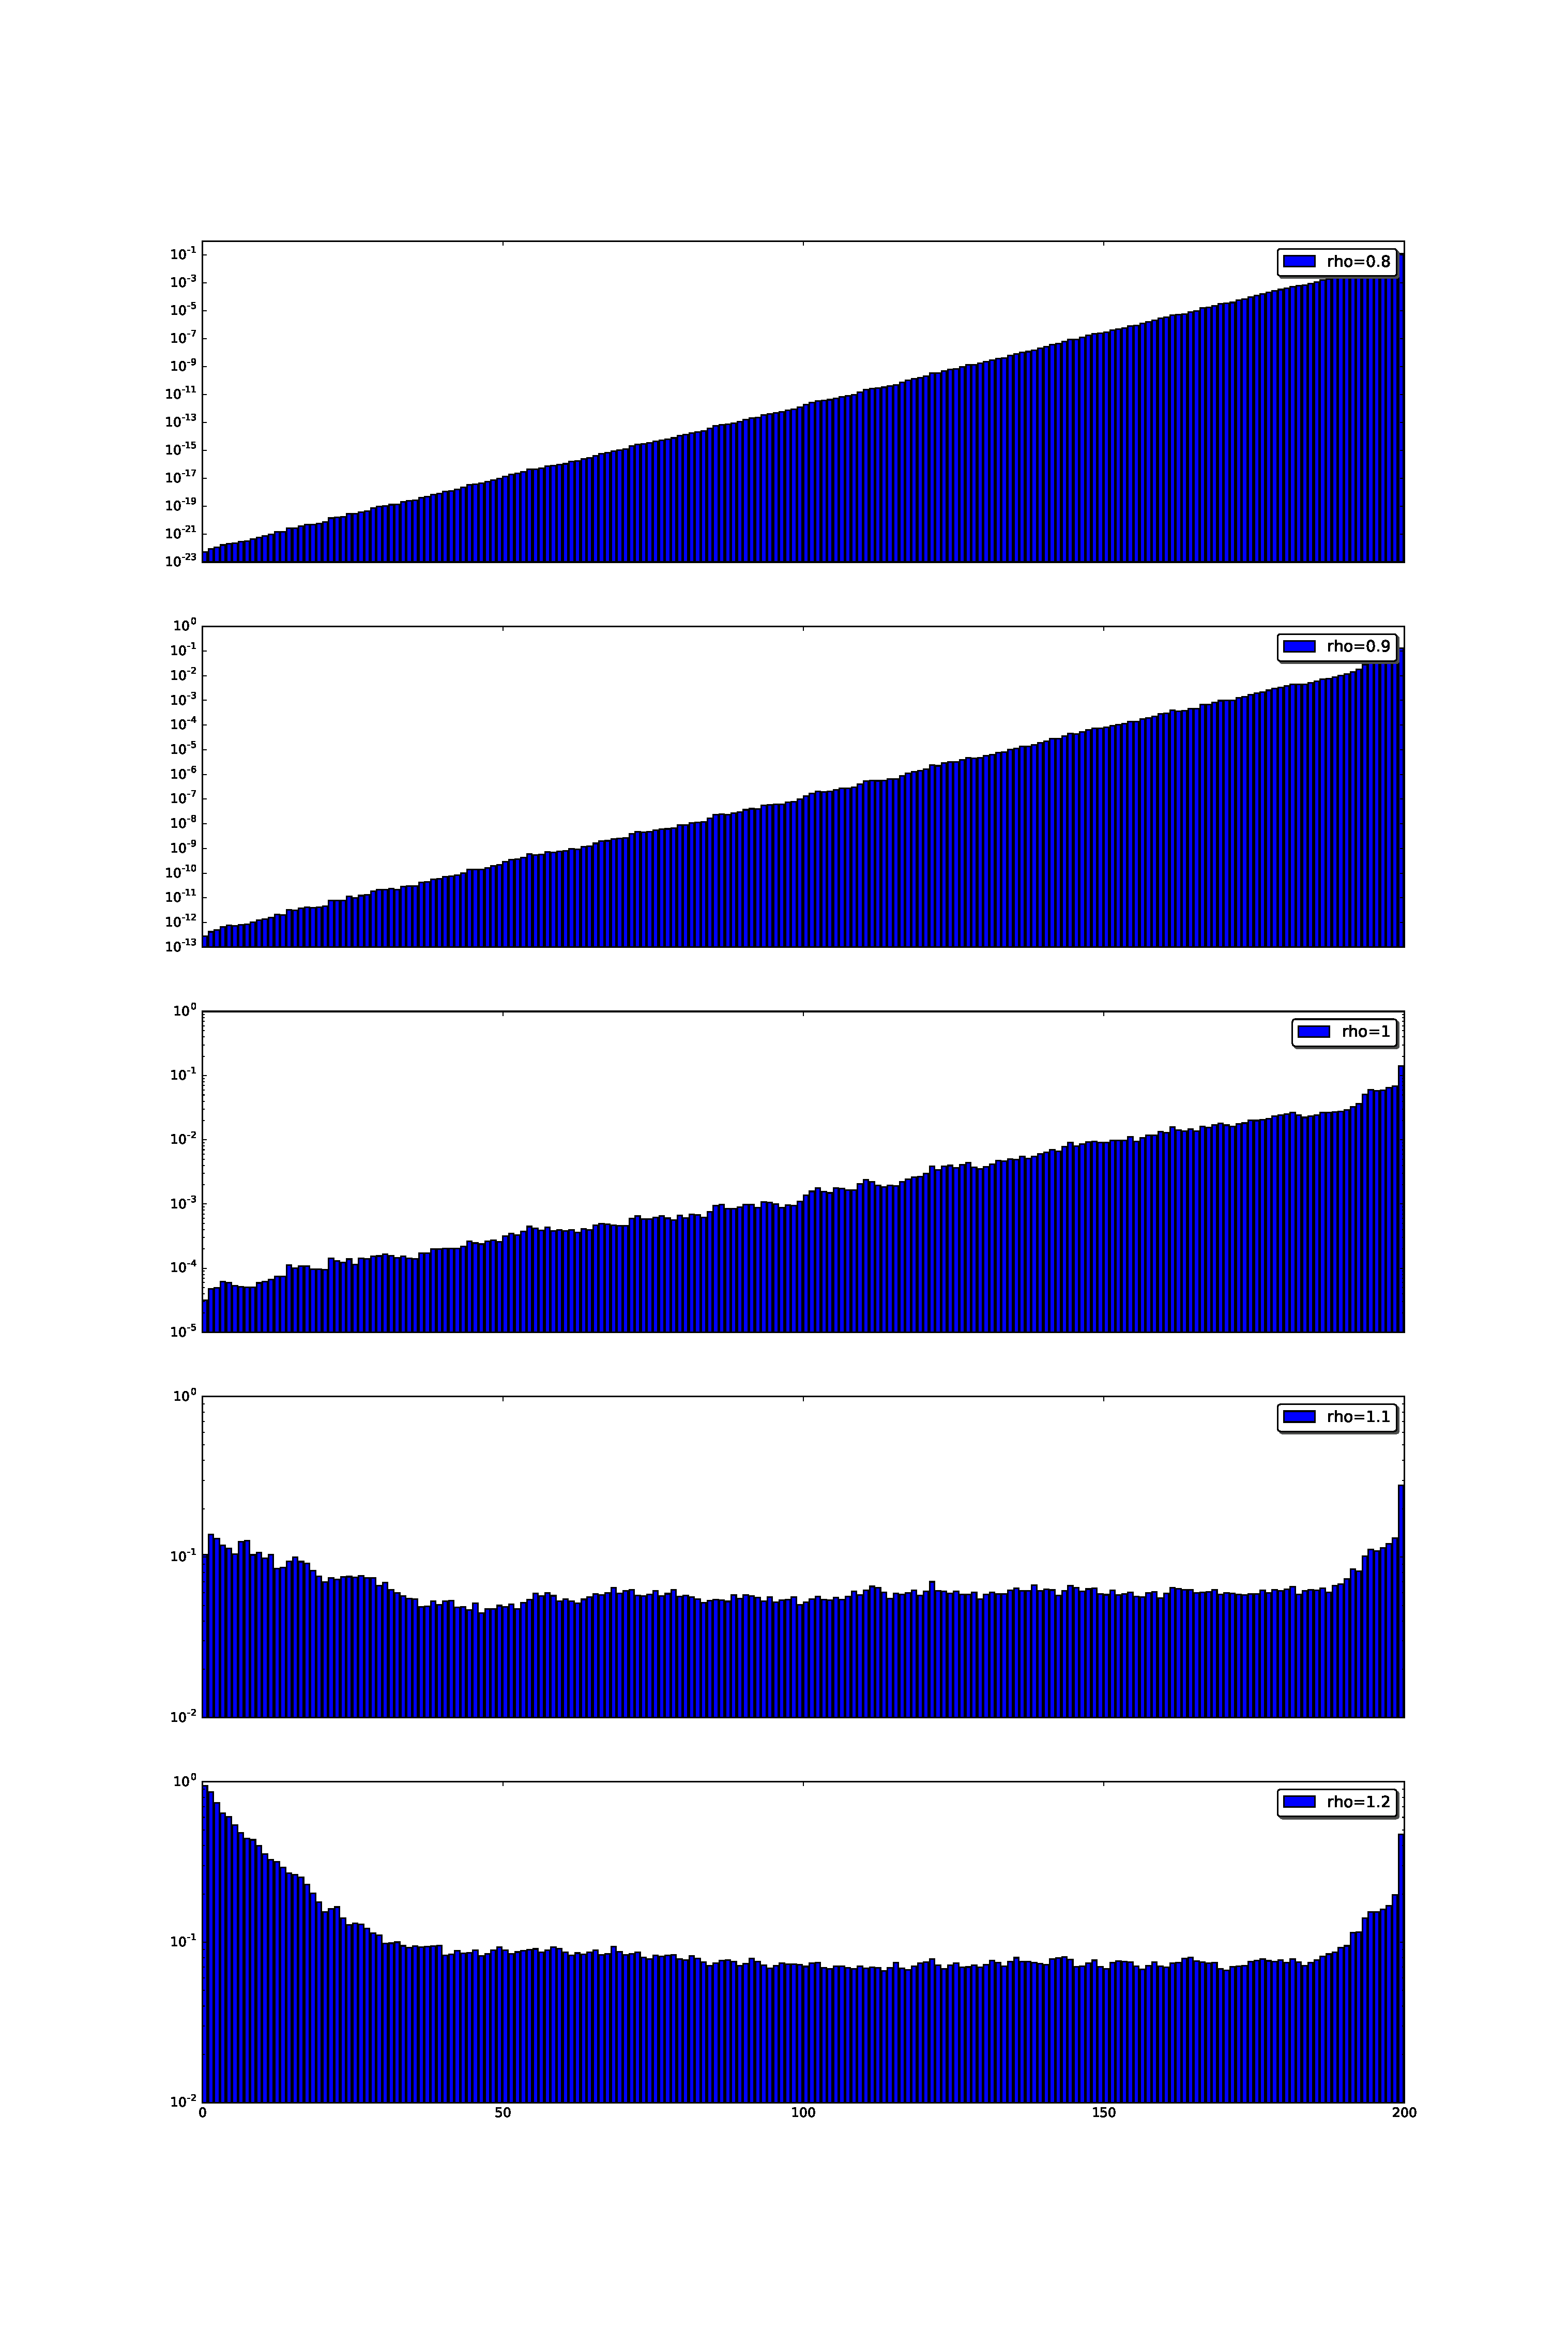
\includegraphics[width=0.9\textwidth]{chapter3/temporal_components.eps}
    \caption{Temporal components for the temporal order task varying the spectral radius of the recurrent matrix. y axis is in logarithmic scale.}
    \label{fig:temporal_norms}
\end{figure}

The first two cases, the one with spectral radius less than one, are perfect example of vanishing gradient instances: more recent temporal components have norm exponentially bigger than the more distant ones (please note that the y axis is in logarithmic scale). On the contrary such phenomenon is not observed in the cases of spectral radius bigger than one where the temporal components have roughly the same norm.

We found that, at least in the task we explored (SAY WHICH ONES), an appropriate spectral radius always allow the training process to start in a regime where the gradient does not vanish. We report some results on the effect of the initialization on the training process in chapter \ref{ch:experiments}

\section{Descent direction}

\begin{figure}
	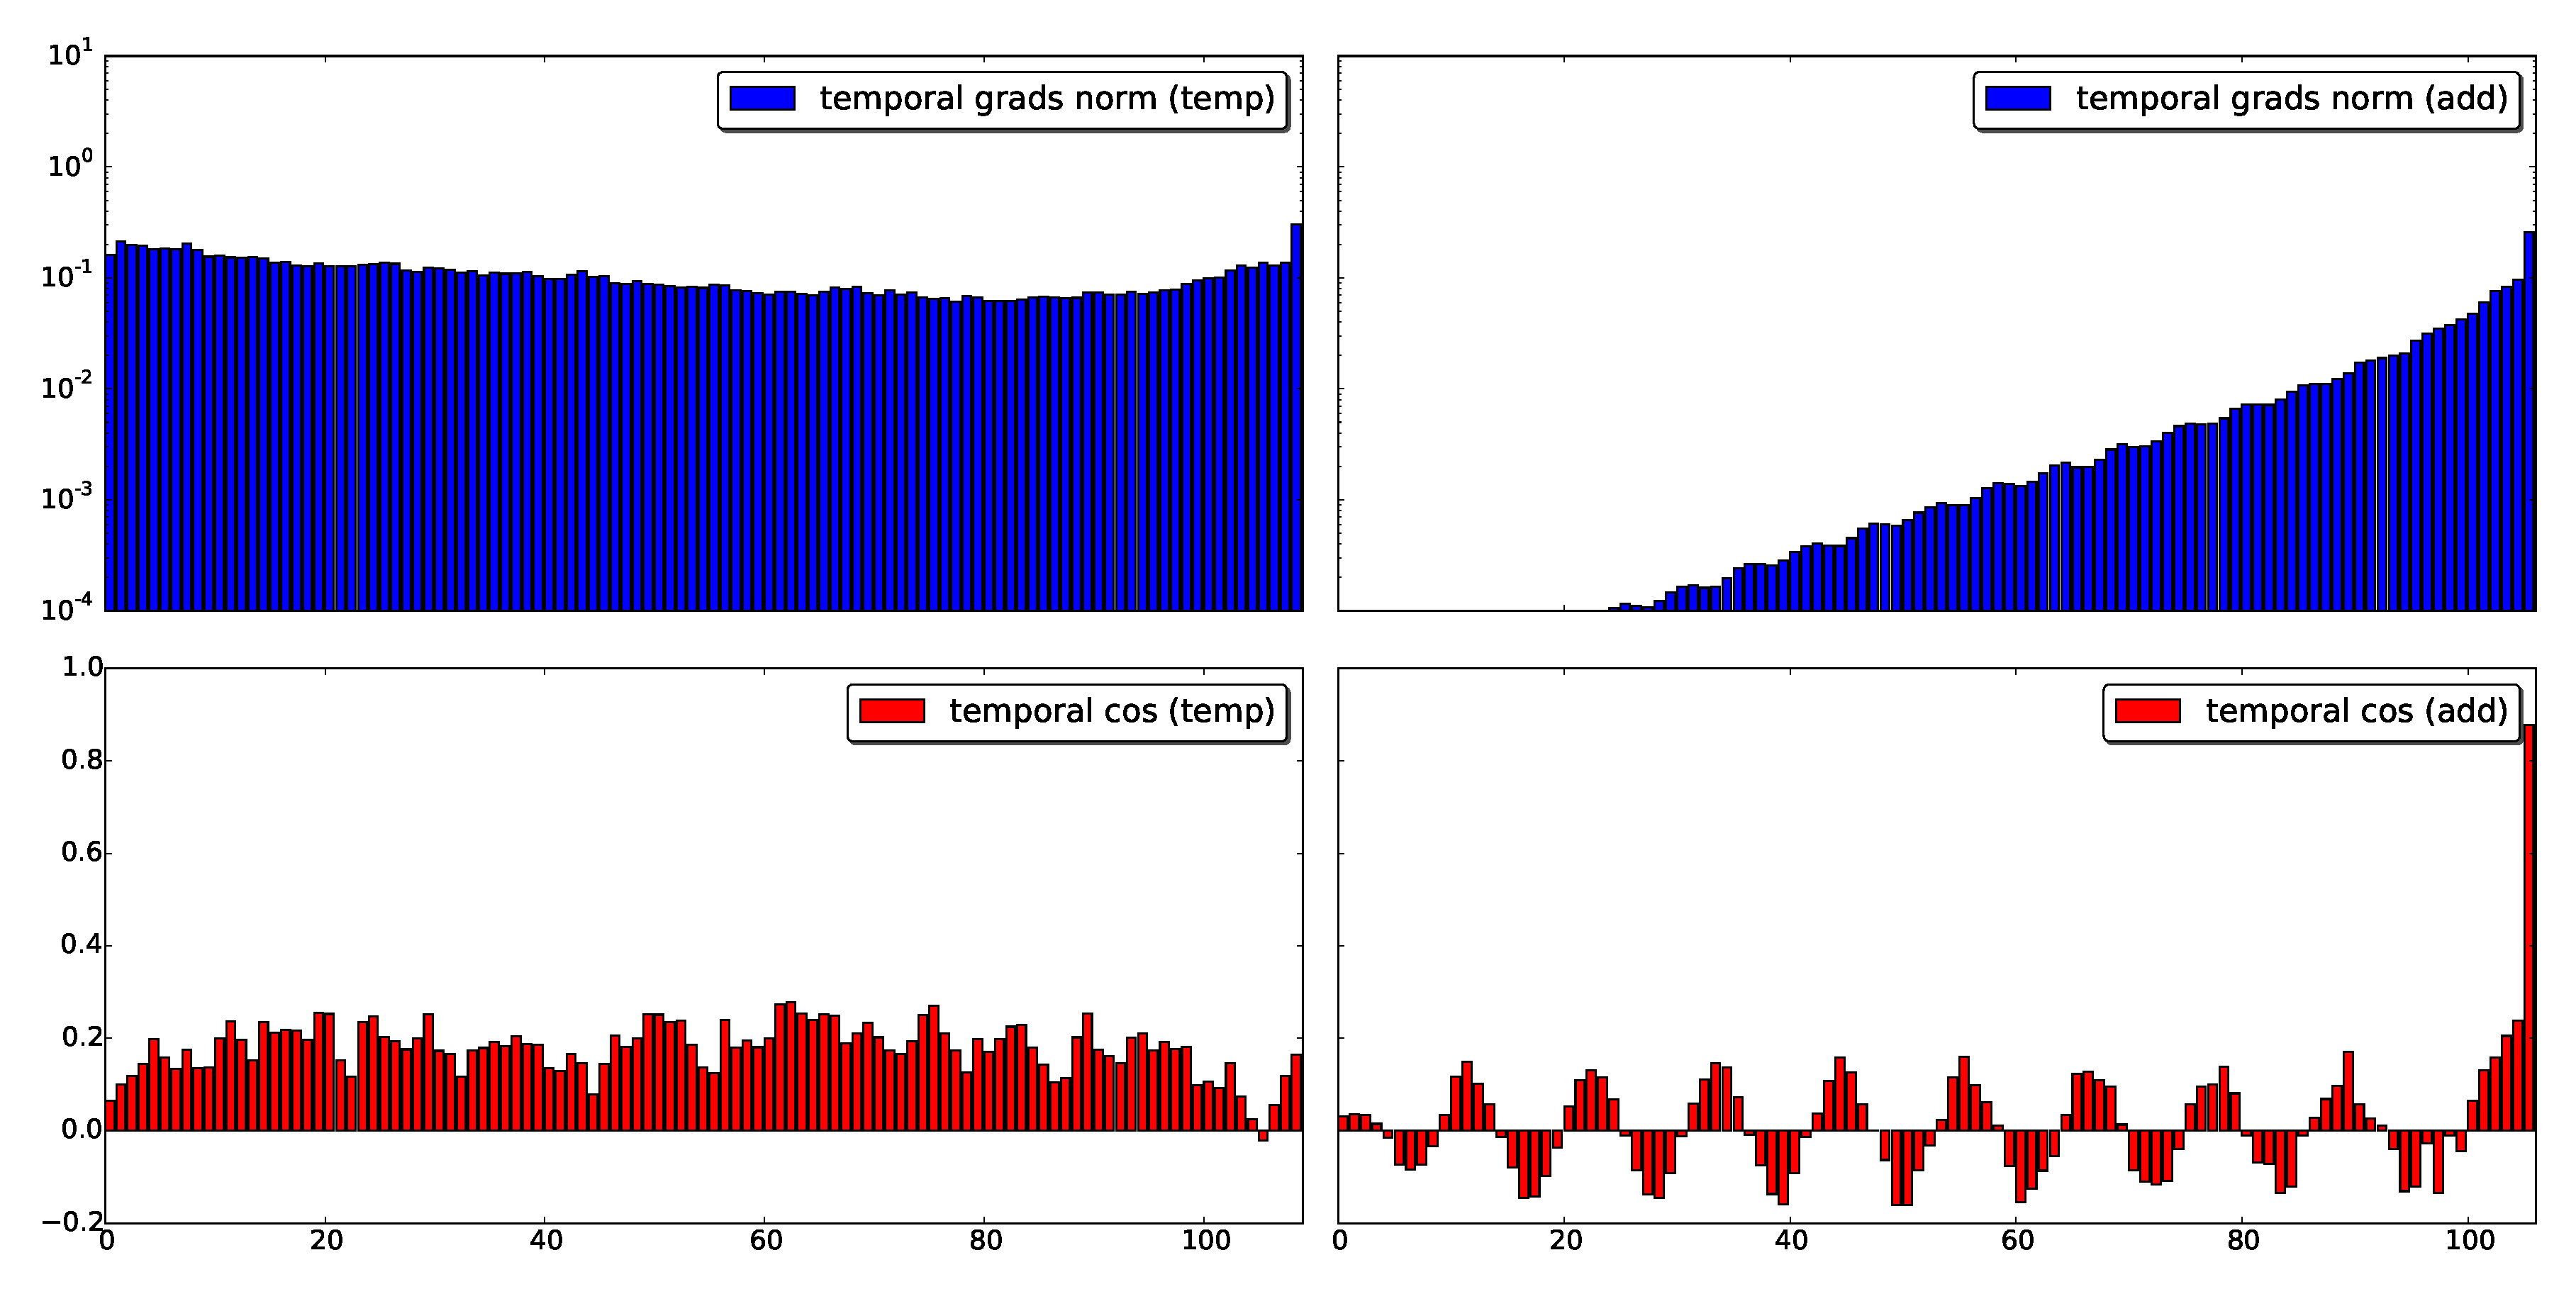
\includegraphics[width=1.4\textwidth]{chapter3/compare_add_temp_norms_1.eps}
	\caption{Temporal components for the temporal order task varying the spectral radius of the recurrent matrix. y axis is in logarithmic scale.}
	\label{fig:}
\end{figure}


The idea is to use the structure of the gradient to compute a "descent" direction which does not suffer from the vanishing problem.

\begin{itemize}
	\item normalize the temporal components:
	\begin{equation}
	g_t(\vec{x}) = \frac{\nabla L_{|t}(\vec{x})}{\norm{\nabla L_{|t}(\vec{x})}}.
	\end{equation}
	
	\item combine the normalized gradients in a simplex:
	\begin{equation}
	g(\vec{x}) = \sum_{t=1}^T \beta_t \cdot g_t(\vec{x}).
	\end{equation}
	
	with $\sum_{t=1}^T\beta_t=1, \beta_t>0$ (randomly picked at each iteration).
	\item exploit the gradient norm:
	\begin{equation}
	d(\vec{x}) = \norm{\nabla L (\vec{x})}\frac{g(\vec{x})}{\norm{g(\vec{x})}}.
	\end{equation}
\end{itemize}
\section{Learning rate}

The choice of the learning rate is crucial for the success of the training procedure. It is well known that RNNs give rise to gradients which change extremely fast in norm (the exploding gradient problem). This makes choosing a single constant step, or even designing an adaptive strategy, very difficult, at the least, for this kind of models. A simple trick which allow to choose a fixed step from the beginning is to \textit{clip the gradients}. This technique was introduced and used in slightly different forms in \cite{understandingExplodingGradients} and \cite{clippingMikolov} and we describe it in section \ref{algo:sgd}. We reformulate the version proposed in \cite{understandingExplodingGradients} as a learning rate selection strategy.
Given a direction $\vec{d}_k$ the step $\alpha_k$ is chosen as:
\begin{equation}
\alpha_k = 
\begin{cases}
	\mu  \quad &\mbox{if} \norm{\vec{d}_k}_2 \leq \tau\\
	\frac{\mu \cdot \tau}{\norm{\vec{d}_k}_2} \quad & otherwise,
\end{cases}
\end{equation}
where $\mu$ and $c$ are some positive constants. The parameter $\tau$ is the threshold on the direction norm; $\mu$ is instead the constant learning rate that is used when the norm of the direction is not above such threshold. The idea is to use a constant step when the direction has an enough small norm and vice-versa choose a step which inversely proportional when such norm is too big. We confirm, as found in works cited above, that this trick is essential to train RNNs in a stochastic framework.

\section{Putting all togheter}
TODO

\section{Proof of convergence}
 
\documentclass{article}
\usepackage[utf8]{inputenc}
\usepackage[italian]{babel}
\usepackage{graphicx}
\usepackage{cite}
\usepackage[hidelinks]{hyperref}
\usepackage{listings}
\usepackage{latexsym}
\usepackage{amsmath}
\usepackage{proof}
\usepackage{stmaryrd}
\usepackage{amssymb}
\usepackage{epstopdf}
\usepackage{pgf}
\usepackage{tikz}
\usepackage[noend]{algpseudocode}
\usepackage[ruled,noline,linesnumbered]{algorithm2e}
\usetikzlibrary{automata,arrows}
\let\emptyset\varnothing

\graphicspath{ {./images/} }

%%Notation:

%%vectors
\renewcommand{\vec}[1]{\boldsymbol{#1}}
%%sets
\newcommand{\set}[1]{\mathcal{#1}}
%%matrixes
\newcommand{\mat}[1]{#1}
%%norm
\newcommand{\norm}[1]{\left\Vert #1 \right\Vert}
%%defeq
\newcommand{\defeq}{\triangleq}
%%
\newcommand{\net}[1]{\mathrm{#1}}
%% pair<x,y>
\newcommand{\pair}[2]{\langle#1,#2\rangle}

\title{Stochastic gradient descent}
\author{Giulio Galvan}

\begin{document}
	\maketitle
\noindent
Consider the stochastic optimization problem 
\begin{equation}
	\underset{\vec{x} \in \mathbb{R}^n}{\text{min}} f(\vec{x}) = \mathbb{E[F(\vec{x}, \vec{\xi})]},
	\label{eq:stochastic_prob}
\end{equation}
where $\vec{\xi} \in \Omega \subset \mathbb{R}^d$ is a random vector.
Suppose $f(\cdot)$ is continuous, strongly convex (with constant $c$) and there exists a compact level set of $f(\cdot)$, hence (\ref{eq:stochastic_prob}) has a unique optimal solution $\vec{x}_*$. Let also $L$ be the Lipschitz constant of $\nabla f$.
We make the following two assumptions:
\begin{itemize}
	\item	It is possible to generate independent identically distributed samples of $\vec{\xi}$
	\item There exists an oracle which, for a given point $(\vec{x}, \vec{\xi})$ return a stochastic descent direction $D(\vec{x}, \vec{\xi})$ such that $d(\vec{x})\defeq\mathbb{E}[D(\vec{x}, \vec{\xi})]$ satisfies:
	\begin{equation}
	-(\vec{x}-\vec{x}_*)^T (\nabla f(\vec{x}) -g(\vec{x})) \geq -\mu L \norm{\vec{x}_j-\vec{x}_*}^2_2\quad \forall \vec{x} \in \mathbb{R}^n,
	\label{eq:angular_condition}
	\end{equation}
	for some $\mu \in (0,\frac{c}{L}) $.
\end{itemize}
Consider the algorithm defined by
\begin{equation}
	\vec{x}_{j+1} = \vec{x}_j -\gamma_j D(\vec{x}_j,\vec{\xi}_j).
	\label{eq:stochastic_algo}
\end{equation}
Each iterate $\vec{x}_j$ of such random process is a function of the history $\vec{\xi}_{[j-1]}=(\vec{\xi}_1,\dots, \vec{\xi}_{j-1})$

Let $A_j\defeq \norm{\vec{x}_j-\vec{x}_*}^2_2$ and $a_j\defeq\mathbb{E}[A_j]$.
From (\ref*{eq:stochastic_algo}) we get
\begin{equation}
\begin{aligned}
	A_{j+1} &= \frac{1}{2}\norm{\vec{x}_j - \gamma_jD(\vec{x}_j,\vec{\xi}_j) -\vec{x}_*}^2_2\\ 
	&= A_j +\frac{1}{2}\gamma_j^2\norm{D(\vec{x}_j,\vec{\xi}_j)}^2_2 - \gamma_j(\vec{x}_j-\vec{x}_*)^TD(\vec{x}_j,\vec{\xi}_j).
\end{aligned}
\label{eq:aj_rec}
\end{equation}
Since $\vec{x}_j = \vec{x}_j(\vec{\xi_{[j-1]}})$ is independent of $\vec{\xi}_j$ we have
\begin{equation}
\begin{aligned}
	\mathbb{E}_{\vec{\xi}_{[j]}}[(\vec{x}_j-\vec{x}_*)^TD(\vec{x}_j,\vec{\xi}_j)] &= \mathbb{E}_{\vec{\xi}_{[j-1]}}[\mathbb{E}_{\vec{\xi}_{[j]}}[(\vec{x}_j-\vec{x}_*)^TD(\vec{x}_j,\vec{\xi}_j)]|\vec{\xi}_{[j-1]}]\\
	&= \mathbb{E}_{\vec{\xi}_{[j-1]}}[(\vec{x}_j-\vec{x}_*)^T\mathbb{E}{\vec{\xi}_{[j]}}[D(\vec{x}_j,\vec{\xi}_j)]|\vec{\xi}_{[j-1]}]\\
	&=\mathbb{E}_{\vec{\xi}_{[j-1]}}[(\vec{x}_j-\vec{x}_*)^Td(\vec{x}_j)]\\
\end{aligned}
\label{eq:independece}
\end{equation}
Let now assume that there exists $M>0$ such that
\begin{equation}
	\mathbb{E}[\norm{D(\vec{x},\vec{\xi})}^2_2]\leq M^2 \quad \forall \vec{x} \in \mathbb{R}^n.
	\label{eq:gradient_bound}
\end{equation}
Using (\ref{eq:independece}) and (\ref{eq:gradient_bound}) we obtain, taking expectation of both sides of (\ref{eq:aj_rec})
\begin{equation}
	a_{j+1} \leq a_j - \gamma_j\mathbb{E}_{\vec{\xi}_{[j-1]}}[(\vec{x}_j-\vec{x}_*)^Td(\vec{x}_j)] + \frac{1}{2}\gamma_j^2M^2
	\label{eq:aj_rec_2}
\end{equation}
Since $f(\cdot)$ is strongly convex there exists $c>0$ such that
\begin{equation}
	(\vec{y}-\vec{x})^T(\nabla f(\vec{y})- \nabla f(\vec{x}))\geq c \norm{\vec{y}-\vec{x}}^2_2
	\label{eq:strong_convexity}
\end{equation}
By optimality of $\vec{x}_*$ we have
\begin{equation}
	(\vec{x}-\vec{x}_*)^T\nabla f(\vec{x}_*) \geq 0 \quad \vec{x} \in \mathbb{R}^n.
	\label{eq:optimality}
\end{equation}
Inequalities (\ref{eq:optimality}) and (\ref{eq:strong_convexity}) implies
\begin{equation}
	(\vec{x}-\vec{x}_*)^T \nabla f(\vec{x}) \geq c \norm{\vec{x}-\vec{x}_*}^2_2 \quad \vec{x} \in \mathbb{R}^n.
\end{equation}
Adding and subtracting the descent direction $g(\vec{x})$ we get
\begin{equation}
	(\vec{x}-\vec{x}_*)^T (\nabla f(\vec{x}) -g(\vec{x}) +g(\vec{x})) \geq c \norm{\vec{x}-\vec{x}_*}^2_2,
\end{equation}
which can be rewritten as
\begin{equation}
		(\vec{x}-\vec{x}_*)^T g(\vec{x}) \geq c \norm{\vec{x}-\vec{x}_*}^2_2 - (\vec{x}-\vec{x}_*)^T (\nabla f(\vec{x}) -g(\vec{x}))
		\label{eq:angular_inequality}
\end{equation}
From assumption (\ref{eq:angular_condition}), taking expectations of both side of (\ref{eq:angular_inequality}) we obtain
\begin{align}
\mathbb{E}[(\vec{x}_j-\vec{x}_*)^T g(\vec{x}_j)] &\geq c \mathbb{E}[\norm{\vec{x}_j-\vec{x}_*}^2_2)] - \mathbb{E}[(\vec{x}_j-\vec{x}_*)^T (\nabla f(\vec{x}_j) -g(\vec{x}_j))]\\
 &\geq c(1-\frac{\mu L}{c}) \mathbb{E}[\norm{\vec{x}_j-\vec{x}_*}^2_2)]\\
 & = 2\bar{c}a_j,
\end{align}
with $\bar{c}=c(1-\frac{\mu L}{c})$.
Hence from (\ref{eq:aj_rec_2}) follows 
\begin{equation}
	a_{j+1} \leq (1-2\bar{c}\gamma_j)a_j + \frac{1}{2}\gamma_j^2M^2.
\end{equation}
Choosing the stepsizes as $\gamma_j = \frac{\beta}{j}$ for some constant $\beta>\frac{1}{2\bar{c}}$ we get
\begin{equation}
		a_{j+1} \leq (1-2\bar{c}\gamma_j)a_j + \frac{1}{2}\frac{\beta^2M^2}{j^2}.
\end{equation}
It follows by induction that
\begin{equation}
	\mathbb{E}[\norm{\vec{x}_j - \vec{x}_*}^2_2] = 2a_j\leq \frac{Q(\beta)}{j},
\end{equation}
where 
\begin{equation}
	Q(\beta) = max\left\{\frac{\beta^2M^2}{2\bar{c}-1},\norm{\vec{x}_1 - \vec{x}_*}^2_2 \right\}.
\end{equation}
Hence, since
\begin{equation}
	f(\vec{x})\leq f(\vec{x}_*) + \frac{1}{2}L\norm{\vec{x} - \vec{x}_*}^2_2, \quad \forall \vec{x} \in \mathbb{R}^n,
\end{equation}
we obtain
\begin{equation}
	\mathbb{E}[f(\vec{x}_j)-f(\vec{x}_*)] \leq \frac{1}{2} L \mathbb{E}[\norm{\vec{x}_j - \vec{x}_*}^2_2] \leq \frac{1}{2}LQ(\beta)
\end{equation}

\paragraph{Sufficient descent direction condition} Assumption \ref{eq:angular_condition} can be further elaborated.
Let $\theta$ be the angle between $\nabla f(\vec{x})$ and $g(\vec{x})$ and $\norm{g(\vec{x})} = \alpha \norm{\nabla f(\vec{x})}$ for some $\alpha>0$.
Then,
\begin{align}
	\norm{\nabla f(\vec{x}_j)-g(\vec{x}_j)}^2 &= \norm{\nabla f(\vec{x}_j)}^2 + \norm{g(\vec{x}_j)}^2 -2\norm{\nabla f(\vec{x}_j)}\norm{g(\vec{x}_j)}\cos\theta_j\\
	&=  \norm{\nabla f(\vec{x}_j)}^2(1+\alpha_j^2-2\alpha_j \cos\theta_j).
\end{align}
Since $\nabla f(\vec{x}_*)=0$, using Lipschitz continuity of $\nabla f$ (with constant L) we get
\begin{equation}
	\norm{\nabla f(\vec{x}_j)-g(\vec{x})} \leq L\norm{\vec{x}-\vec{x}_*} (1+\alpha^2-2\alpha \cos\theta)^{\frac{1}{2}}
\end{equation}
Hence
\begin{align}
(\vec{x}-\vec{x}_*)^T (\nabla f(\vec{x}) -g(\vec{x})) &\leq \norm{\vec{x}-\vec{x}_*} \norm{\nabla f(\vec{x}) -g(\vec{x})}\\
&\leq L\norm{\vec{x}-\vec{x}_*}^2 (1+\alpha^2-2\alpha \cos\theta)^{\frac{1}{2}}.
\end{align}
Hence a sufficient condition for assumption \ref{eq:angular_condition} to hold is
\begin{equation}
	1+\alpha^2-2\alpha \cos\theta_j\leq \mu^2
\end{equation}

\end{document}      




\section{A new SGD approach for training RNNs}
\begin{frame}{Initialization}
	
The matrix $\mat{W}^{rec}$ is \textbf{scaled} to have a desired spectral radius.

\vspace{2em}

\begin{algorithm}[H]
	\KwData{\\
		\Indp
		$\rho = $ desired spectral radius
	}
	\BlankLine
	
	$\mat{W_{rec}} \sim \mathcal{N}(0, \sigma^2)$\\
	$r \gets \mbox{spectral\_radius}(\mat{W_{rec}})$\\
	$\mat{W_{rec}}\gets \frac{\rho}{r} \cdot \mat{W_{rec}}$\\
	\KwRet{$\mat{W_{rec}}$}
	\caption{Recurrent weight matrix initialization scheme}
	\label{algo:init_scaling}
\end{algorithm}
\end{frame}

\begin{frame}{The effect of initialization on the temporal gradients}
	\captionsetup[subfigure]{labelformat=empty}
		\begin{figure}
			\centering
			\subfloat[][]{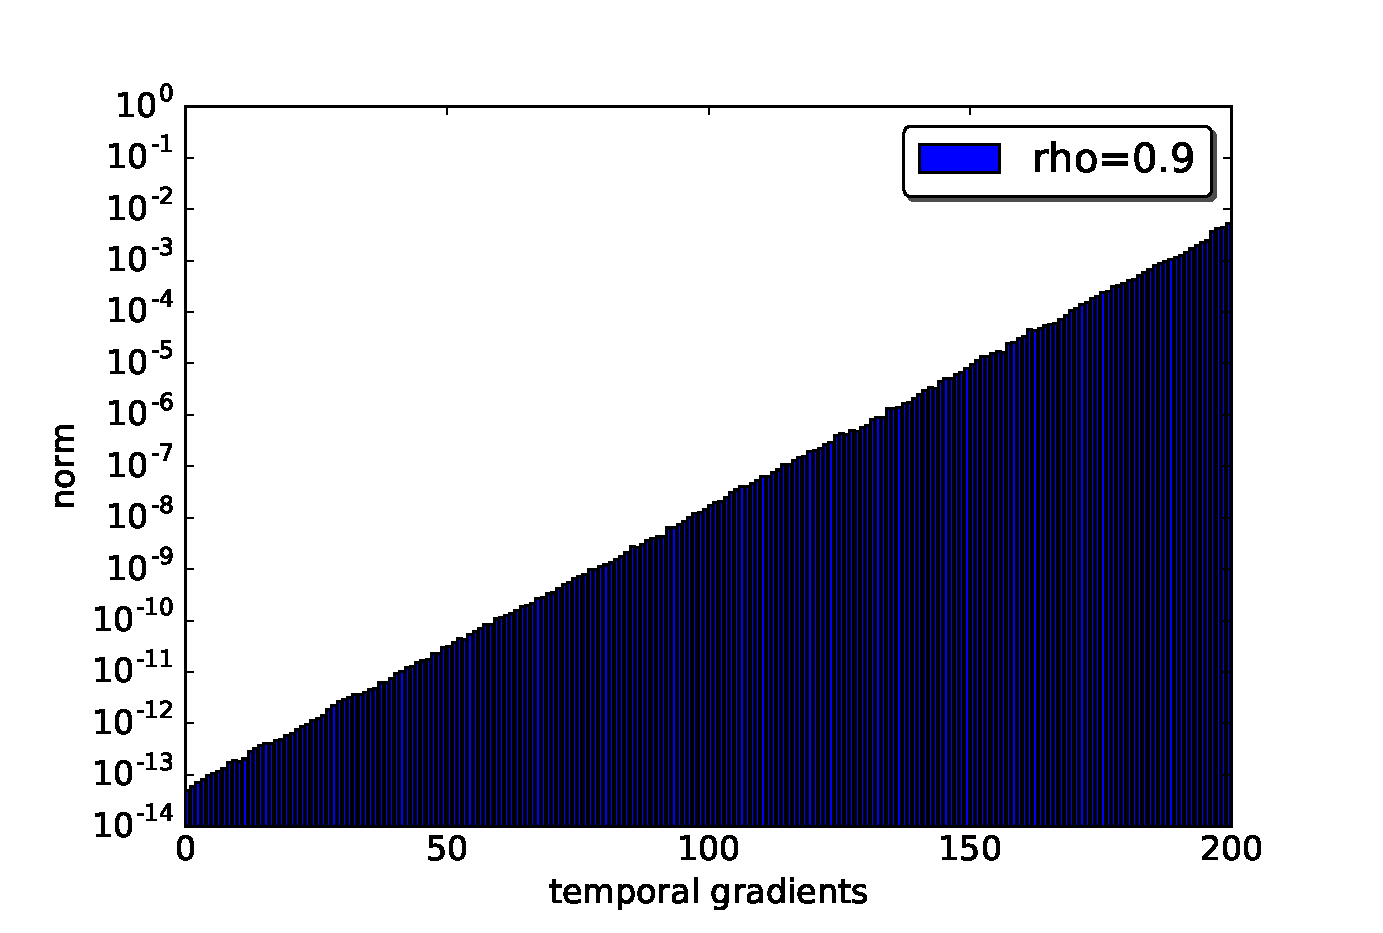
\includegraphics[width= 0.5\textwidth]{plot_grad_norms_it0_09.eps}\label{fig:temp_norms_09}}
			\subfloat[][]{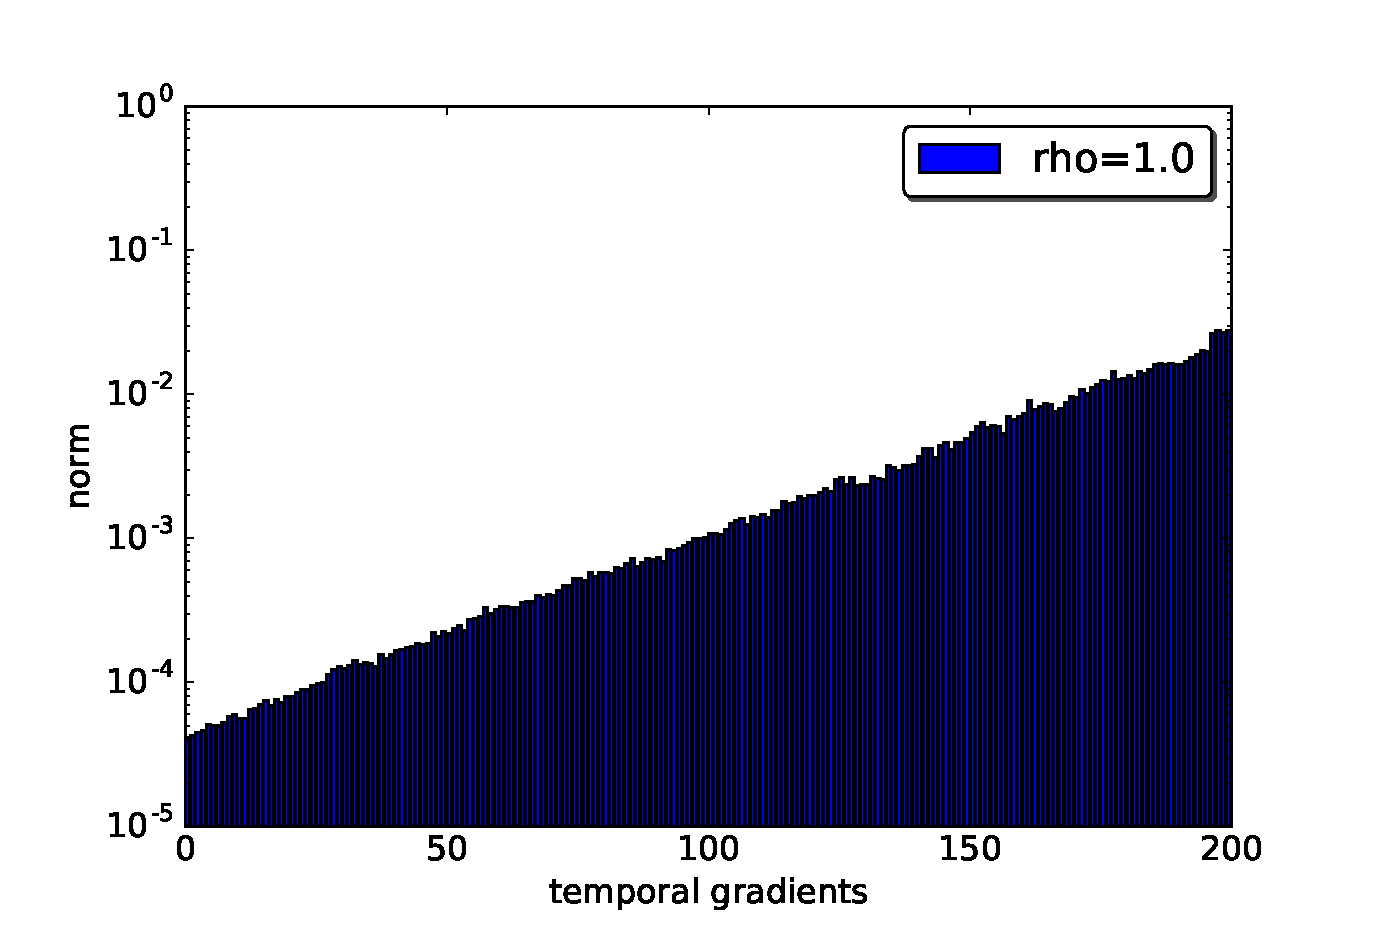
\includegraphics[width= 0.5\textwidth]{plot_grad_norms_it0_1.eps}\label{fig:temp_norms_1}}\\
			\vspace{-2em}
			\subfloat[][]{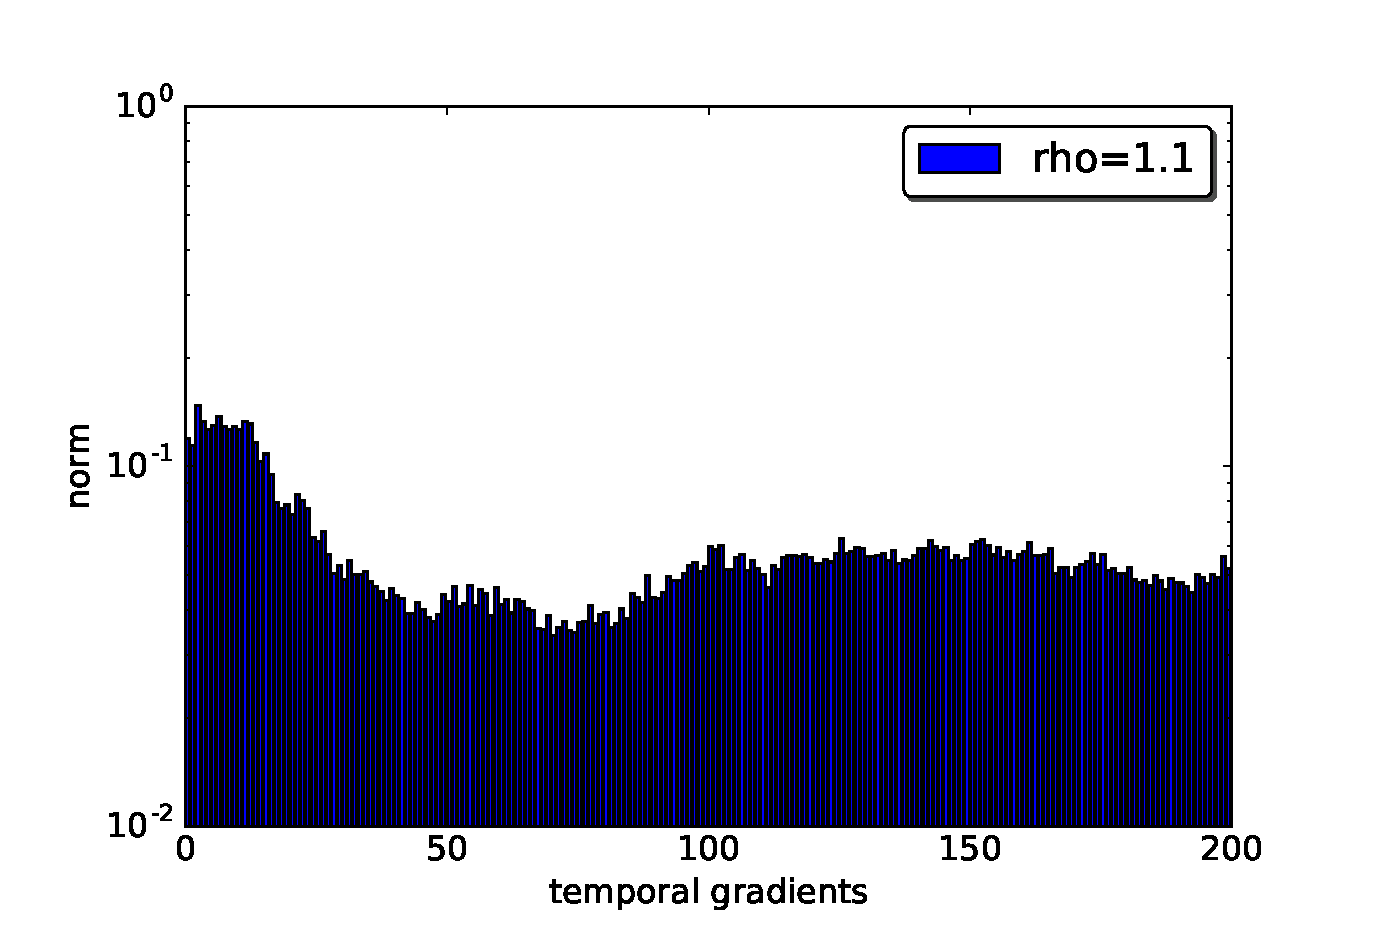
\includegraphics[width= 0.5\textwidth]{plot_grad_norms_it0_11.eps}\label{fig:temp_norms_11}}
			\subfloat[][]{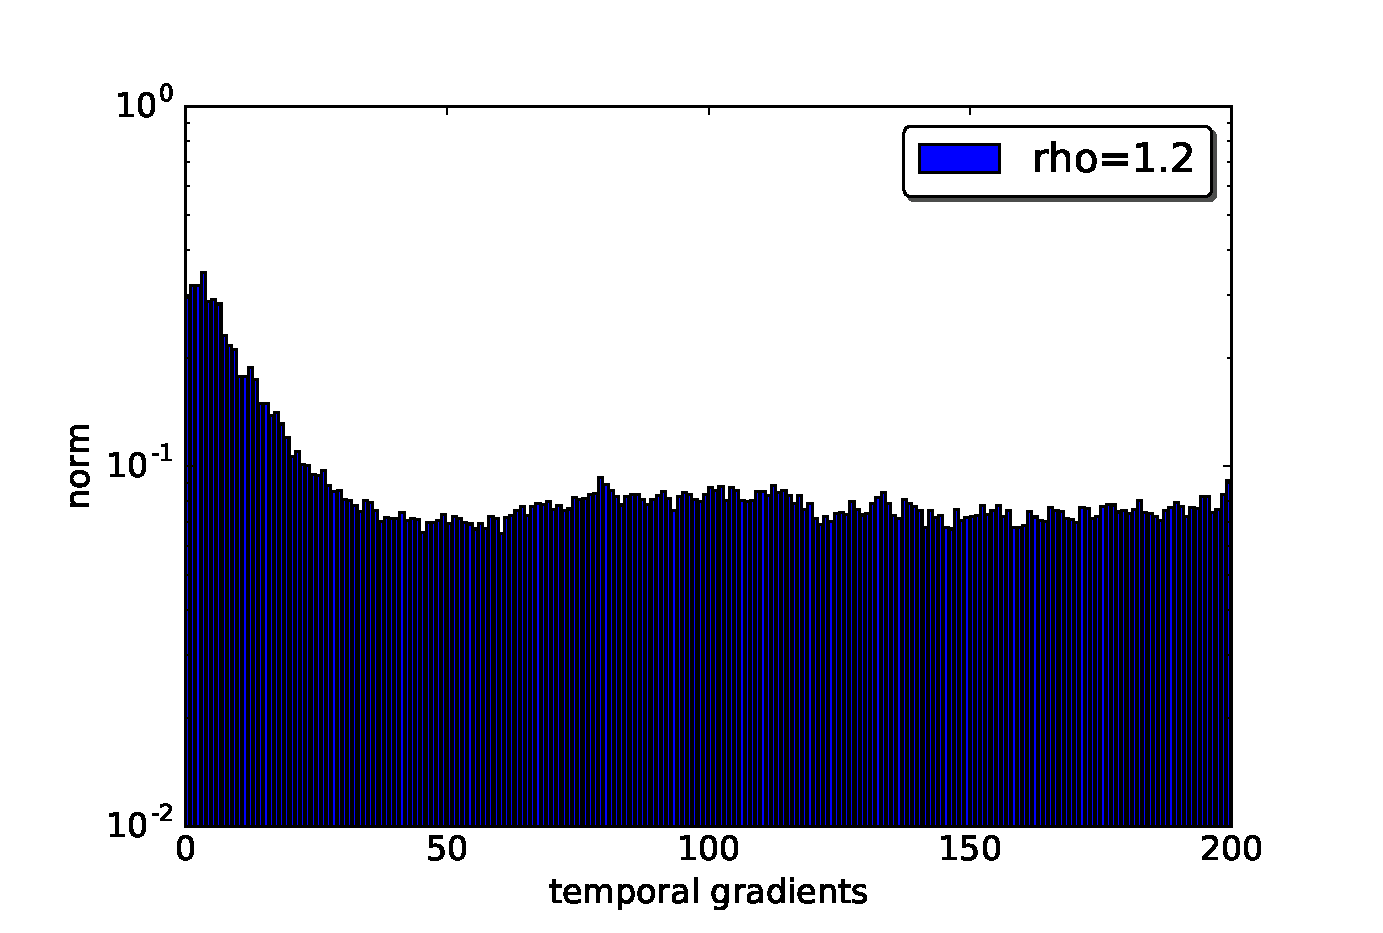
\includegraphics[width= 0.5\textwidth]{plot_grad_norms_it0_12.eps}\label{fig:temp_norms_12}}
		\end{figure}
	
%	\vspace{-3em}
%	\begin{figure}[H]
%		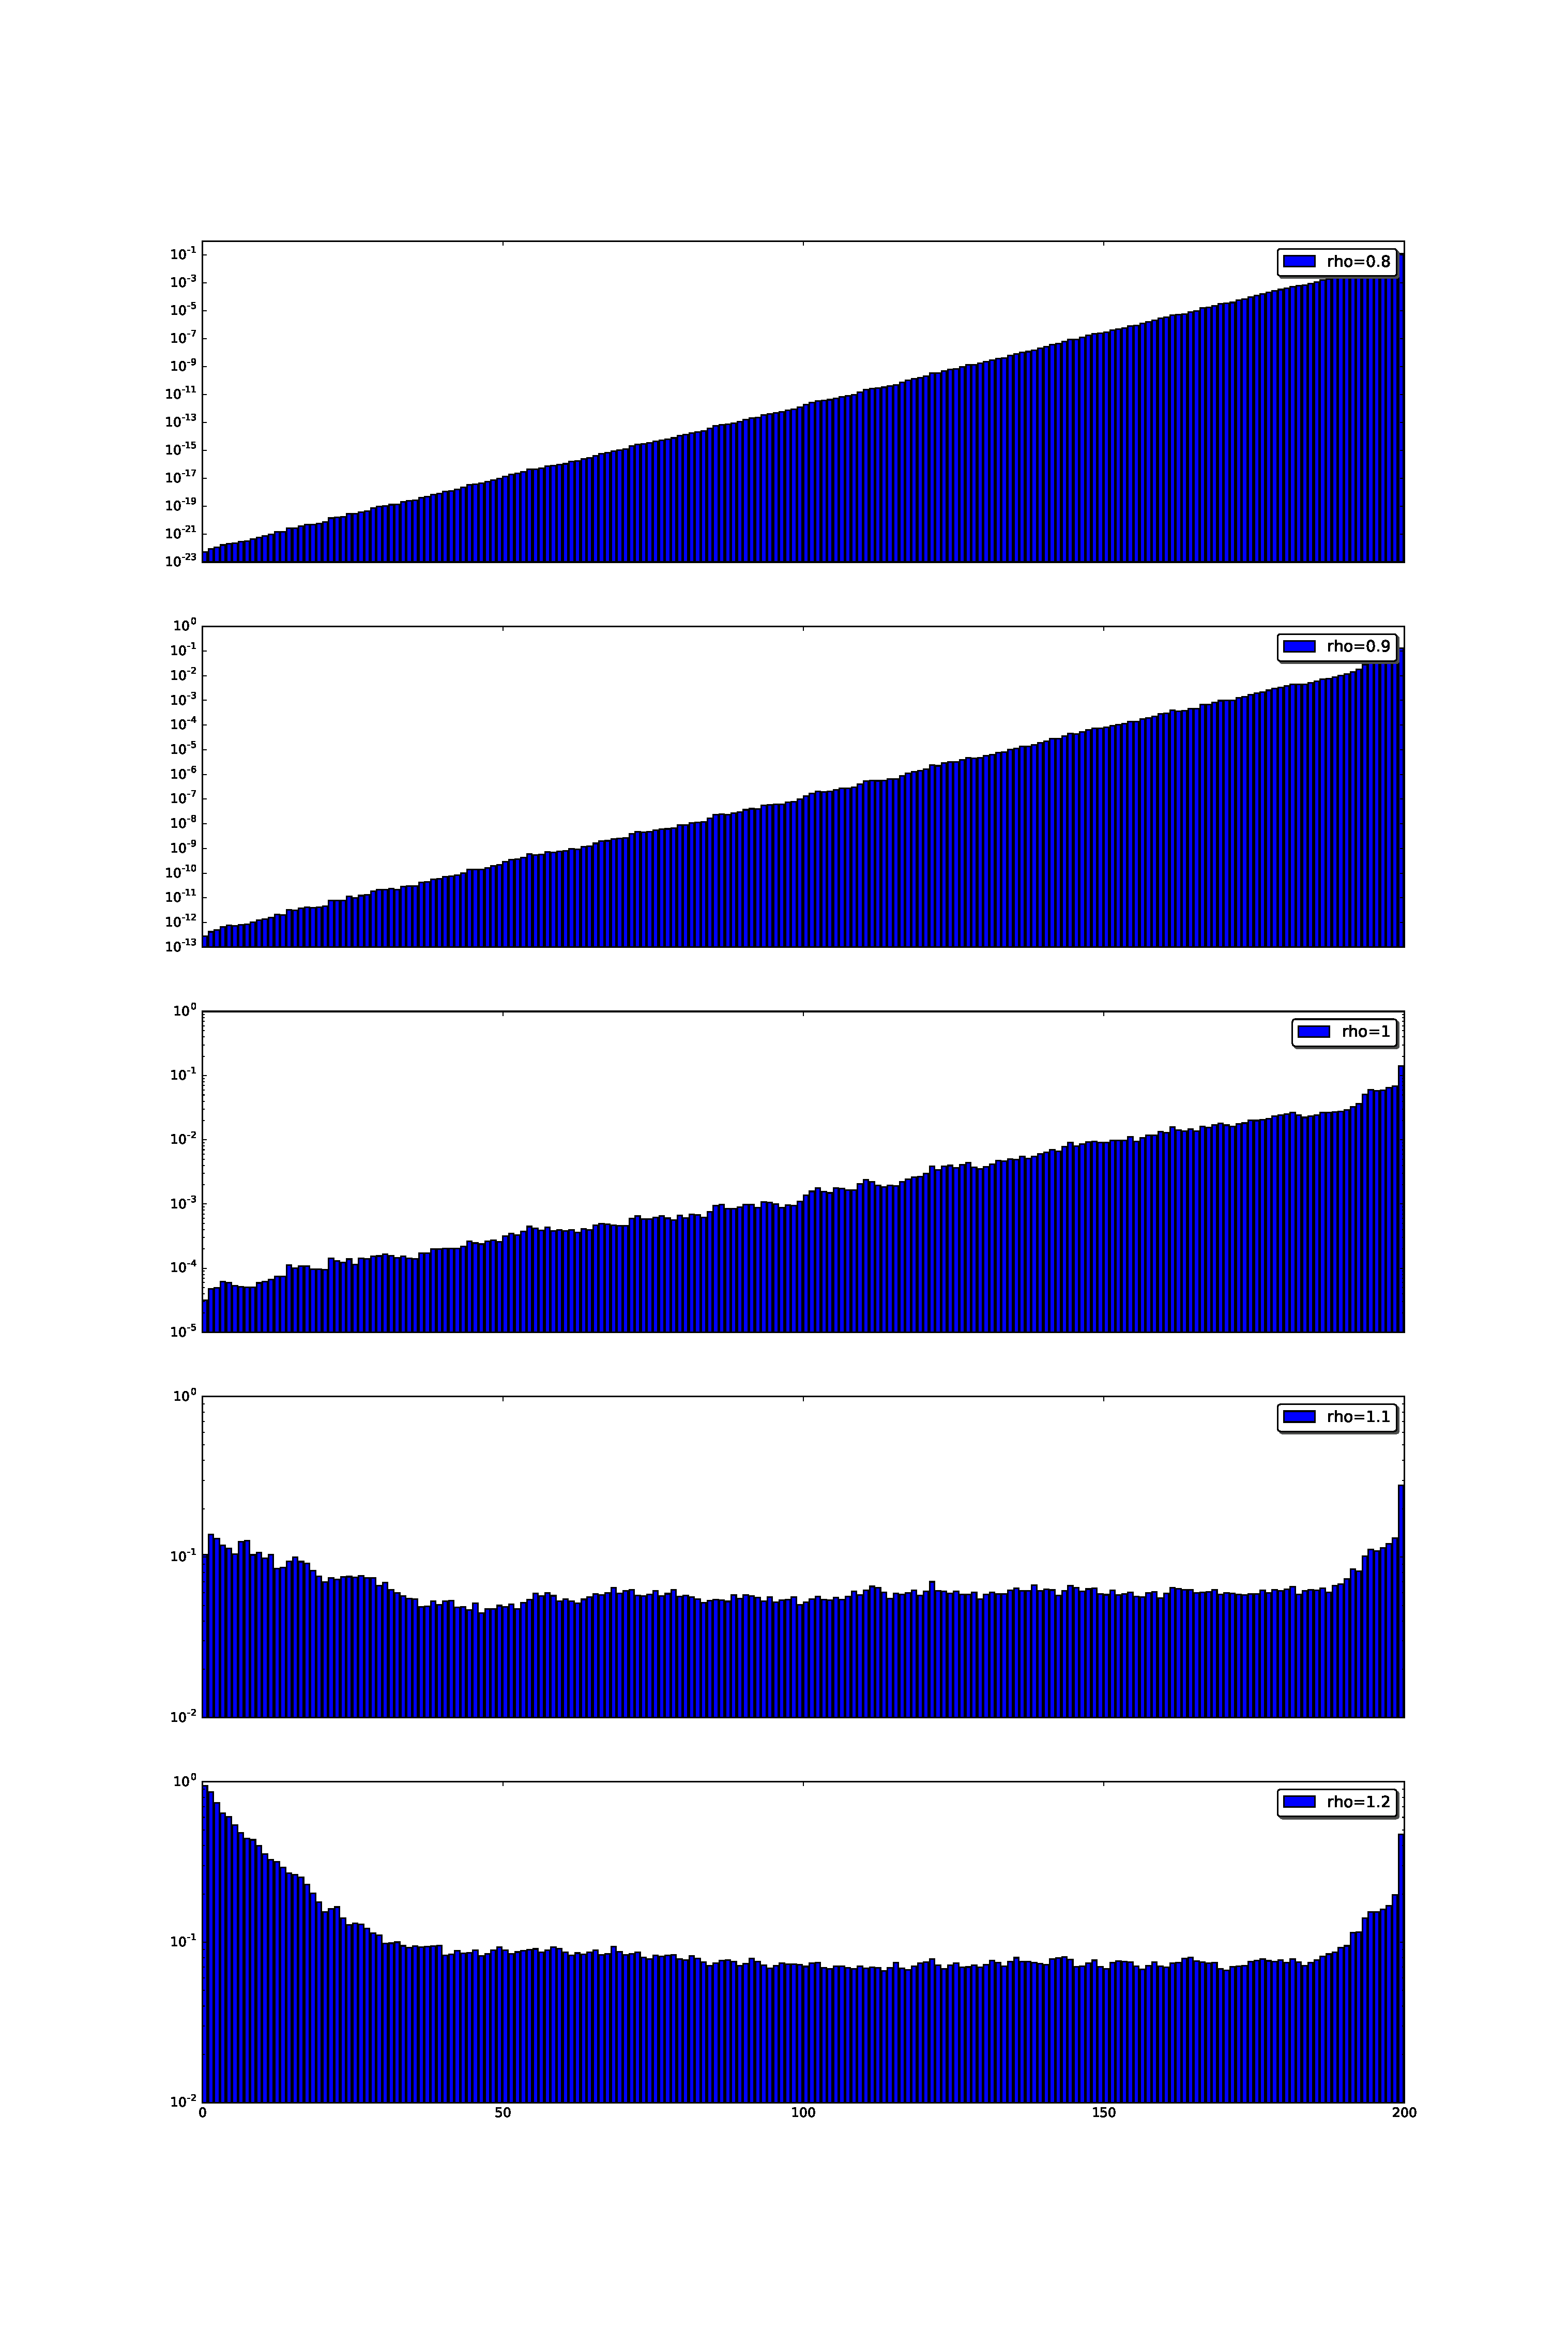
\includegraphics[width=0.6\textwidth]{temporal_components_rho.eps}
%		\caption{Temporal gradients for the temporal order task varying the spectral radius of the recurrent matrix. y axis is in logarithmic scale.}
%		\label{fig:temporal_norms}
%	\end{figure}
\end{frame}

\begin{frame}{The effect of initialization on the rate of success}
	\begin{figure}
		\centering
%		%% Creator: Matplotlib, PGF backend
%%
%% To include the figure in your LaTeX document, write
%%   \input{<filename>.pgf}
%%
%% Make sure the required packages are loaded in your preamble
%%   \usepackage{pgf}
%%
%% Figures using additional raster images can only be included by \input if
%% they are in the same directory as the main LaTeX file. For loading figures
%% from other directories you can use the `import` package
%%   \usepackage{import}
%% and then include the figures with
%%   \import{<path to file>}{<filename>.pgf}
%%
%% Matplotlib used the following preamble
%%   \usepackage{fontspec}
%%   \setmainfont{DejaVu Serif}
%%   \setsansfont{DejaVu Sans}
%%   \setmonofont{DejaVu Sans Mono}
%%
\begingroup%
\makeatletter%
\begin{pgfpicture}%
\pgfpathrectangle{\pgfpointorigin}{\pgfqpoint{8.000000in}{6.000000in}}%
\pgfusepath{use as bounding box, clip}%
\begin{pgfscope}%
\pgfsetbuttcap%
\pgfsetmiterjoin%
\definecolor{currentfill}{rgb}{1.000000,1.000000,1.000000}%
\pgfsetfillcolor{currentfill}%
\pgfsetlinewidth{0.000000pt}%
\definecolor{currentstroke}{rgb}{1.000000,1.000000,1.000000}%
\pgfsetstrokecolor{currentstroke}%
\pgfsetdash{}{0pt}%
\pgfpathmoveto{\pgfqpoint{0.000000in}{0.000000in}}%
\pgfpathlineto{\pgfqpoint{8.000000in}{0.000000in}}%
\pgfpathlineto{\pgfqpoint{8.000000in}{6.000000in}}%
\pgfpathlineto{\pgfqpoint{0.000000in}{6.000000in}}%
\pgfpathclose%
\pgfusepath{fill}%
\end{pgfscope}%
\begin{pgfscope}%
\pgfsetbuttcap%
\pgfsetmiterjoin%
\definecolor{currentfill}{rgb}{1.000000,1.000000,1.000000}%
\pgfsetfillcolor{currentfill}%
\pgfsetlinewidth{0.000000pt}%
\definecolor{currentstroke}{rgb}{0.000000,0.000000,0.000000}%
\pgfsetstrokecolor{currentstroke}%
\pgfsetstrokeopacity{0.000000}%
\pgfsetdash{}{0pt}%
\pgfpathmoveto{\pgfqpoint{1.000000in}{0.600000in}}%
\pgfpathlineto{\pgfqpoint{7.200000in}{0.600000in}}%
\pgfpathlineto{\pgfqpoint{7.200000in}{5.400000in}}%
\pgfpathlineto{\pgfqpoint{1.000000in}{5.400000in}}%
\pgfpathclose%
\pgfusepath{fill}%
\end{pgfscope}%
\begin{pgfscope}%
\pgfpathrectangle{\pgfqpoint{1.000000in}{0.600000in}}{\pgfqpoint{6.200000in}{4.800000in}} %
\pgfusepath{clip}%
\pgfsetbuttcap%
\pgfsetroundjoin%
\pgfsetlinewidth{1.003750pt}%
\definecolor{currentstroke}{rgb}{0.000000,0.000000,1.000000}%
\pgfsetstrokecolor{currentstroke}%
\pgfsetdash{{6.000000pt}{6.000000pt}}{0.000000pt}%
\pgfpathmoveto{\pgfqpoint{1.281818in}{5.000000in}}%
\pgfpathlineto{\pgfqpoint{1.563636in}{5.000000in}}%
\pgfpathlineto{\pgfqpoint{2.409091in}{5.000000in}}%
\pgfpathlineto{\pgfqpoint{3.818182in}{3.640000in}}%
\pgfpathlineto{\pgfqpoint{5.227273in}{3.640000in}}%
\pgfpathlineto{\pgfqpoint{6.636364in}{1.000000in}}%
\pgfusepath{stroke}%
\end{pgfscope}%
\begin{pgfscope}%
\pgfpathrectangle{\pgfqpoint{1.000000in}{0.600000in}}{\pgfqpoint{6.200000in}{4.800000in}} %
\pgfusepath{clip}%
\pgfsetbuttcap%
\pgfsetroundjoin%
\definecolor{currentfill}{rgb}{0.000000,0.000000,1.000000}%
\pgfsetfillcolor{currentfill}%
\pgfsetlinewidth{0.501875pt}%
\definecolor{currentstroke}{rgb}{0.000000,0.000000,0.000000}%
\pgfsetstrokecolor{currentstroke}%
\pgfsetdash{}{0pt}%
\pgfsys@defobject{currentmarker}{\pgfqpoint{-0.041667in}{-0.041667in}}{\pgfqpoint{0.041667in}{0.041667in}}{%
\pgfpathmoveto{\pgfqpoint{0.000000in}{-0.041667in}}%
\pgfpathcurveto{\pgfqpoint{0.011050in}{-0.041667in}}{\pgfqpoint{0.021649in}{-0.037276in}}{\pgfqpoint{0.029463in}{-0.029463in}}%
\pgfpathcurveto{\pgfqpoint{0.037276in}{-0.021649in}}{\pgfqpoint{0.041667in}{-0.011050in}}{\pgfqpoint{0.041667in}{0.000000in}}%
\pgfpathcurveto{\pgfqpoint{0.041667in}{0.011050in}}{\pgfqpoint{0.037276in}{0.021649in}}{\pgfqpoint{0.029463in}{0.029463in}}%
\pgfpathcurveto{\pgfqpoint{0.021649in}{0.037276in}}{\pgfqpoint{0.011050in}{0.041667in}}{\pgfqpoint{0.000000in}{0.041667in}}%
\pgfpathcurveto{\pgfqpoint{-0.011050in}{0.041667in}}{\pgfqpoint{-0.021649in}{0.037276in}}{\pgfqpoint{-0.029463in}{0.029463in}}%
\pgfpathcurveto{\pgfqpoint{-0.037276in}{0.021649in}}{\pgfqpoint{-0.041667in}{0.011050in}}{\pgfqpoint{-0.041667in}{0.000000in}}%
\pgfpathcurveto{\pgfqpoint{-0.041667in}{-0.011050in}}{\pgfqpoint{-0.037276in}{-0.021649in}}{\pgfqpoint{-0.029463in}{-0.029463in}}%
\pgfpathcurveto{\pgfqpoint{-0.021649in}{-0.037276in}}{\pgfqpoint{-0.011050in}{-0.041667in}}{\pgfqpoint{0.000000in}{-0.041667in}}%
\pgfpathclose%
\pgfusepath{stroke,fill}%
}%
\begin{pgfscope}%
\pgfsys@transformshift{1.281818in}{5.000000in}%
\pgfsys@useobject{currentmarker}{}%
\end{pgfscope}%
\begin{pgfscope}%
\pgfsys@transformshift{1.563636in}{5.000000in}%
\pgfsys@useobject{currentmarker}{}%
\end{pgfscope}%
\begin{pgfscope}%
\pgfsys@transformshift{2.409091in}{5.000000in}%
\pgfsys@useobject{currentmarker}{}%
\end{pgfscope}%
\begin{pgfscope}%
\pgfsys@transformshift{3.818182in}{3.640000in}%
\pgfsys@useobject{currentmarker}{}%
\end{pgfscope}%
\begin{pgfscope}%
\pgfsys@transformshift{5.227273in}{3.640000in}%
\pgfsys@useobject{currentmarker}{}%
\end{pgfscope}%
\begin{pgfscope}%
\pgfsys@transformshift{6.636364in}{1.000000in}%
\pgfsys@useobject{currentmarker}{}%
\end{pgfscope}%
\end{pgfscope}%
\begin{pgfscope}%
\pgfpathrectangle{\pgfqpoint{1.000000in}{0.600000in}}{\pgfqpoint{6.200000in}{4.800000in}} %
\pgfusepath{clip}%
\pgfsetbuttcap%
\pgfsetroundjoin%
\pgfsetlinewidth{1.003750pt}%
\definecolor{currentstroke}{rgb}{1.000000,0.000000,0.000000}%
\pgfsetstrokecolor{currentstroke}%
\pgfsetdash{{6.000000pt}{6.000000pt}}{0.000000pt}%
\pgfpathmoveto{\pgfqpoint{1.281818in}{5.000000in}}%
\pgfpathlineto{\pgfqpoint{1.563636in}{5.000000in}}%
\pgfpathlineto{\pgfqpoint{2.409091in}{1.000000in}}%
\pgfpathlineto{\pgfqpoint{3.818182in}{1.000000in}}%
\pgfpathlineto{\pgfqpoint{5.227273in}{1.000000in}}%
\pgfpathlineto{\pgfqpoint{6.636364in}{1.000000in}}%
\pgfusepath{stroke}%
\end{pgfscope}%
\begin{pgfscope}%
\pgfpathrectangle{\pgfqpoint{1.000000in}{0.600000in}}{\pgfqpoint{6.200000in}{4.800000in}} %
\pgfusepath{clip}%
\pgfsetbuttcap%
\pgfsetroundjoin%
\definecolor{currentfill}{rgb}{1.000000,0.000000,0.000000}%
\pgfsetfillcolor{currentfill}%
\pgfsetlinewidth{0.501875pt}%
\definecolor{currentstroke}{rgb}{0.000000,0.000000,0.000000}%
\pgfsetstrokecolor{currentstroke}%
\pgfsetdash{}{0pt}%
\pgfsys@defobject{currentmarker}{\pgfqpoint{-0.041667in}{-0.041667in}}{\pgfqpoint{0.041667in}{0.041667in}}{%
\pgfpathmoveto{\pgfqpoint{0.000000in}{-0.041667in}}%
\pgfpathcurveto{\pgfqpoint{0.011050in}{-0.041667in}}{\pgfqpoint{0.021649in}{-0.037276in}}{\pgfqpoint{0.029463in}{-0.029463in}}%
\pgfpathcurveto{\pgfqpoint{0.037276in}{-0.021649in}}{\pgfqpoint{0.041667in}{-0.011050in}}{\pgfqpoint{0.041667in}{0.000000in}}%
\pgfpathcurveto{\pgfqpoint{0.041667in}{0.011050in}}{\pgfqpoint{0.037276in}{0.021649in}}{\pgfqpoint{0.029463in}{0.029463in}}%
\pgfpathcurveto{\pgfqpoint{0.021649in}{0.037276in}}{\pgfqpoint{0.011050in}{0.041667in}}{\pgfqpoint{0.000000in}{0.041667in}}%
\pgfpathcurveto{\pgfqpoint{-0.011050in}{0.041667in}}{\pgfqpoint{-0.021649in}{0.037276in}}{\pgfqpoint{-0.029463in}{0.029463in}}%
\pgfpathcurveto{\pgfqpoint{-0.037276in}{0.021649in}}{\pgfqpoint{-0.041667in}{0.011050in}}{\pgfqpoint{-0.041667in}{0.000000in}}%
\pgfpathcurveto{\pgfqpoint{-0.041667in}{-0.011050in}}{\pgfqpoint{-0.037276in}{-0.021649in}}{\pgfqpoint{-0.029463in}{-0.029463in}}%
\pgfpathcurveto{\pgfqpoint{-0.021649in}{-0.037276in}}{\pgfqpoint{-0.011050in}{-0.041667in}}{\pgfqpoint{0.000000in}{-0.041667in}}%
\pgfpathclose%
\pgfusepath{stroke,fill}%
}%
\begin{pgfscope}%
\pgfsys@transformshift{1.281818in}{5.000000in}%
\pgfsys@useobject{currentmarker}{}%
\end{pgfscope}%
\begin{pgfscope}%
\pgfsys@transformshift{1.563636in}{5.000000in}%
\pgfsys@useobject{currentmarker}{}%
\end{pgfscope}%
\begin{pgfscope}%
\pgfsys@transformshift{2.409091in}{1.000000in}%
\pgfsys@useobject{currentmarker}{}%
\end{pgfscope}%
\begin{pgfscope}%
\pgfsys@transformshift{3.818182in}{1.000000in}%
\pgfsys@useobject{currentmarker}{}%
\end{pgfscope}%
\begin{pgfscope}%
\pgfsys@transformshift{5.227273in}{1.000000in}%
\pgfsys@useobject{currentmarker}{}%
\end{pgfscope}%
\begin{pgfscope}%
\pgfsys@transformshift{6.636364in}{1.000000in}%
\pgfsys@useobject{currentmarker}{}%
\end{pgfscope}%
\end{pgfscope}%
\begin{pgfscope}%
\pgfsetrectcap%
\pgfsetmiterjoin%
\pgfsetlinewidth{1.003750pt}%
\definecolor{currentstroke}{rgb}{0.000000,0.000000,0.000000}%
\pgfsetstrokecolor{currentstroke}%
\pgfsetdash{}{0pt}%
\pgfpathmoveto{\pgfqpoint{7.200000in}{0.600000in}}%
\pgfpathlineto{\pgfqpoint{7.200000in}{5.400000in}}%
\pgfusepath{stroke}%
\end{pgfscope}%
\begin{pgfscope}%
\pgfsetrectcap%
\pgfsetmiterjoin%
\pgfsetlinewidth{1.003750pt}%
\definecolor{currentstroke}{rgb}{0.000000,0.000000,0.000000}%
\pgfsetstrokecolor{currentstroke}%
\pgfsetdash{}{0pt}%
\pgfpathmoveto{\pgfqpoint{1.000000in}{5.400000in}}%
\pgfpathlineto{\pgfqpoint{7.200000in}{5.400000in}}%
\pgfusepath{stroke}%
\end{pgfscope}%
\begin{pgfscope}%
\pgfsetrectcap%
\pgfsetmiterjoin%
\pgfsetlinewidth{1.003750pt}%
\definecolor{currentstroke}{rgb}{0.000000,0.000000,0.000000}%
\pgfsetstrokecolor{currentstroke}%
\pgfsetdash{}{0pt}%
\pgfpathmoveto{\pgfqpoint{1.000000in}{0.600000in}}%
\pgfpathlineto{\pgfqpoint{7.200000in}{0.600000in}}%
\pgfusepath{stroke}%
\end{pgfscope}%
\begin{pgfscope}%
\pgfsetrectcap%
\pgfsetmiterjoin%
\pgfsetlinewidth{1.003750pt}%
\definecolor{currentstroke}{rgb}{0.000000,0.000000,0.000000}%
\pgfsetstrokecolor{currentstroke}%
\pgfsetdash{}{0pt}%
\pgfpathmoveto{\pgfqpoint{1.000000in}{0.600000in}}%
\pgfpathlineto{\pgfqpoint{1.000000in}{5.400000in}}%
\pgfusepath{stroke}%
\end{pgfscope}%
\begin{pgfscope}%
\pgfsetbuttcap%
\pgfsetroundjoin%
\definecolor{currentfill}{rgb}{0.000000,0.000000,0.000000}%
\pgfsetfillcolor{currentfill}%
\pgfsetlinewidth{0.501875pt}%
\definecolor{currentstroke}{rgb}{0.000000,0.000000,0.000000}%
\pgfsetstrokecolor{currentstroke}%
\pgfsetdash{}{0pt}%
\pgfsys@defobject{currentmarker}{\pgfqpoint{0.000000in}{0.000000in}}{\pgfqpoint{0.000000in}{0.055556in}}{%
\pgfpathmoveto{\pgfqpoint{0.000000in}{0.000000in}}%
\pgfpathlineto{\pgfqpoint{0.000000in}{0.055556in}}%
\pgfusepath{stroke,fill}%
}%
\begin{pgfscope}%
\pgfsys@transformshift{1.281818in}{0.600000in}%
\pgfsys@useobject{currentmarker}{}%
\end{pgfscope}%
\end{pgfscope}%
\begin{pgfscope}%
\pgfsetbuttcap%
\pgfsetroundjoin%
\definecolor{currentfill}{rgb}{0.000000,0.000000,0.000000}%
\pgfsetfillcolor{currentfill}%
\pgfsetlinewidth{0.501875pt}%
\definecolor{currentstroke}{rgb}{0.000000,0.000000,0.000000}%
\pgfsetstrokecolor{currentstroke}%
\pgfsetdash{}{0pt}%
\pgfsys@defobject{currentmarker}{\pgfqpoint{0.000000in}{-0.055556in}}{\pgfqpoint{0.000000in}{0.000000in}}{%
\pgfpathmoveto{\pgfqpoint{0.000000in}{0.000000in}}%
\pgfpathlineto{\pgfqpoint{0.000000in}{-0.055556in}}%
\pgfusepath{stroke,fill}%
}%
\begin{pgfscope}%
\pgfsys@transformshift{1.281818in}{5.400000in}%
\pgfsys@useobject{currentmarker}{}%
\end{pgfscope}%
\end{pgfscope}%
\begin{pgfscope}%
\pgftext[x=1.281818in,y=0.544444in,,top]{\sffamily\fontsize{12.000000}{14.400000}\selectfont 10}%
\end{pgfscope}%
\begin{pgfscope}%
\pgfsetbuttcap%
\pgfsetroundjoin%
\definecolor{currentfill}{rgb}{0.000000,0.000000,0.000000}%
\pgfsetfillcolor{currentfill}%
\pgfsetlinewidth{0.501875pt}%
\definecolor{currentstroke}{rgb}{0.000000,0.000000,0.000000}%
\pgfsetstrokecolor{currentstroke}%
\pgfsetdash{}{0pt}%
\pgfsys@defobject{currentmarker}{\pgfqpoint{0.000000in}{0.000000in}}{\pgfqpoint{0.000000in}{0.055556in}}{%
\pgfpathmoveto{\pgfqpoint{0.000000in}{0.000000in}}%
\pgfpathlineto{\pgfqpoint{0.000000in}{0.055556in}}%
\pgfusepath{stroke,fill}%
}%
\begin{pgfscope}%
\pgfsys@transformshift{1.563636in}{0.600000in}%
\pgfsys@useobject{currentmarker}{}%
\end{pgfscope}%
\end{pgfscope}%
\begin{pgfscope}%
\pgfsetbuttcap%
\pgfsetroundjoin%
\definecolor{currentfill}{rgb}{0.000000,0.000000,0.000000}%
\pgfsetfillcolor{currentfill}%
\pgfsetlinewidth{0.501875pt}%
\definecolor{currentstroke}{rgb}{0.000000,0.000000,0.000000}%
\pgfsetstrokecolor{currentstroke}%
\pgfsetdash{}{0pt}%
\pgfsys@defobject{currentmarker}{\pgfqpoint{0.000000in}{-0.055556in}}{\pgfqpoint{0.000000in}{0.000000in}}{%
\pgfpathmoveto{\pgfqpoint{0.000000in}{0.000000in}}%
\pgfpathlineto{\pgfqpoint{0.000000in}{-0.055556in}}%
\pgfusepath{stroke,fill}%
}%
\begin{pgfscope}%
\pgfsys@transformshift{1.563636in}{5.400000in}%
\pgfsys@useobject{currentmarker}{}%
\end{pgfscope}%
\end{pgfscope}%
\begin{pgfscope}%
\pgftext[x=1.563636in,y=0.544444in,,top]{\sffamily\fontsize{12.000000}{14.400000}\selectfont 20}%
\end{pgfscope}%
\begin{pgfscope}%
\pgfsetbuttcap%
\pgfsetroundjoin%
\definecolor{currentfill}{rgb}{0.000000,0.000000,0.000000}%
\pgfsetfillcolor{currentfill}%
\pgfsetlinewidth{0.501875pt}%
\definecolor{currentstroke}{rgb}{0.000000,0.000000,0.000000}%
\pgfsetstrokecolor{currentstroke}%
\pgfsetdash{}{0pt}%
\pgfsys@defobject{currentmarker}{\pgfqpoint{0.000000in}{0.000000in}}{\pgfqpoint{0.000000in}{0.055556in}}{%
\pgfpathmoveto{\pgfqpoint{0.000000in}{0.000000in}}%
\pgfpathlineto{\pgfqpoint{0.000000in}{0.055556in}}%
\pgfusepath{stroke,fill}%
}%
\begin{pgfscope}%
\pgfsys@transformshift{2.409091in}{0.600000in}%
\pgfsys@useobject{currentmarker}{}%
\end{pgfscope}%
\end{pgfscope}%
\begin{pgfscope}%
\pgfsetbuttcap%
\pgfsetroundjoin%
\definecolor{currentfill}{rgb}{0.000000,0.000000,0.000000}%
\pgfsetfillcolor{currentfill}%
\pgfsetlinewidth{0.501875pt}%
\definecolor{currentstroke}{rgb}{0.000000,0.000000,0.000000}%
\pgfsetstrokecolor{currentstroke}%
\pgfsetdash{}{0pt}%
\pgfsys@defobject{currentmarker}{\pgfqpoint{0.000000in}{-0.055556in}}{\pgfqpoint{0.000000in}{0.000000in}}{%
\pgfpathmoveto{\pgfqpoint{0.000000in}{0.000000in}}%
\pgfpathlineto{\pgfqpoint{0.000000in}{-0.055556in}}%
\pgfusepath{stroke,fill}%
}%
\begin{pgfscope}%
\pgfsys@transformshift{2.409091in}{5.400000in}%
\pgfsys@useobject{currentmarker}{}%
\end{pgfscope}%
\end{pgfscope}%
\begin{pgfscope}%
\pgftext[x=2.409091in,y=0.544444in,,top]{\sffamily\fontsize{12.000000}{14.400000}\selectfont 50}%
\end{pgfscope}%
\begin{pgfscope}%
\pgfsetbuttcap%
\pgfsetroundjoin%
\definecolor{currentfill}{rgb}{0.000000,0.000000,0.000000}%
\pgfsetfillcolor{currentfill}%
\pgfsetlinewidth{0.501875pt}%
\definecolor{currentstroke}{rgb}{0.000000,0.000000,0.000000}%
\pgfsetstrokecolor{currentstroke}%
\pgfsetdash{}{0pt}%
\pgfsys@defobject{currentmarker}{\pgfqpoint{0.000000in}{0.000000in}}{\pgfqpoint{0.000000in}{0.055556in}}{%
\pgfpathmoveto{\pgfqpoint{0.000000in}{0.000000in}}%
\pgfpathlineto{\pgfqpoint{0.000000in}{0.055556in}}%
\pgfusepath{stroke,fill}%
}%
\begin{pgfscope}%
\pgfsys@transformshift{3.818182in}{0.600000in}%
\pgfsys@useobject{currentmarker}{}%
\end{pgfscope}%
\end{pgfscope}%
\begin{pgfscope}%
\pgfsetbuttcap%
\pgfsetroundjoin%
\definecolor{currentfill}{rgb}{0.000000,0.000000,0.000000}%
\pgfsetfillcolor{currentfill}%
\pgfsetlinewidth{0.501875pt}%
\definecolor{currentstroke}{rgb}{0.000000,0.000000,0.000000}%
\pgfsetstrokecolor{currentstroke}%
\pgfsetdash{}{0pt}%
\pgfsys@defobject{currentmarker}{\pgfqpoint{0.000000in}{-0.055556in}}{\pgfqpoint{0.000000in}{0.000000in}}{%
\pgfpathmoveto{\pgfqpoint{0.000000in}{0.000000in}}%
\pgfpathlineto{\pgfqpoint{0.000000in}{-0.055556in}}%
\pgfusepath{stroke,fill}%
}%
\begin{pgfscope}%
\pgfsys@transformshift{3.818182in}{5.400000in}%
\pgfsys@useobject{currentmarker}{}%
\end{pgfscope}%
\end{pgfscope}%
\begin{pgfscope}%
\pgftext[x=3.818182in,y=0.544444in,,top]{\sffamily\fontsize{12.000000}{14.400000}\selectfont 100}%
\end{pgfscope}%
\begin{pgfscope}%
\pgfsetbuttcap%
\pgfsetroundjoin%
\definecolor{currentfill}{rgb}{0.000000,0.000000,0.000000}%
\pgfsetfillcolor{currentfill}%
\pgfsetlinewidth{0.501875pt}%
\definecolor{currentstroke}{rgb}{0.000000,0.000000,0.000000}%
\pgfsetstrokecolor{currentstroke}%
\pgfsetdash{}{0pt}%
\pgfsys@defobject{currentmarker}{\pgfqpoint{0.000000in}{0.000000in}}{\pgfqpoint{0.000000in}{0.055556in}}{%
\pgfpathmoveto{\pgfqpoint{0.000000in}{0.000000in}}%
\pgfpathlineto{\pgfqpoint{0.000000in}{0.055556in}}%
\pgfusepath{stroke,fill}%
}%
\begin{pgfscope}%
\pgfsys@transformshift{5.227273in}{0.600000in}%
\pgfsys@useobject{currentmarker}{}%
\end{pgfscope}%
\end{pgfscope}%
\begin{pgfscope}%
\pgfsetbuttcap%
\pgfsetroundjoin%
\definecolor{currentfill}{rgb}{0.000000,0.000000,0.000000}%
\pgfsetfillcolor{currentfill}%
\pgfsetlinewidth{0.501875pt}%
\definecolor{currentstroke}{rgb}{0.000000,0.000000,0.000000}%
\pgfsetstrokecolor{currentstroke}%
\pgfsetdash{}{0pt}%
\pgfsys@defobject{currentmarker}{\pgfqpoint{0.000000in}{-0.055556in}}{\pgfqpoint{0.000000in}{0.000000in}}{%
\pgfpathmoveto{\pgfqpoint{0.000000in}{0.000000in}}%
\pgfpathlineto{\pgfqpoint{0.000000in}{-0.055556in}}%
\pgfusepath{stroke,fill}%
}%
\begin{pgfscope}%
\pgfsys@transformshift{5.227273in}{5.400000in}%
\pgfsys@useobject{currentmarker}{}%
\end{pgfscope}%
\end{pgfscope}%
\begin{pgfscope}%
\pgftext[x=5.227273in,y=0.544444in,,top]{\sffamily\fontsize{12.000000}{14.400000}\selectfont 150}%
\end{pgfscope}%
\begin{pgfscope}%
\pgfsetbuttcap%
\pgfsetroundjoin%
\definecolor{currentfill}{rgb}{0.000000,0.000000,0.000000}%
\pgfsetfillcolor{currentfill}%
\pgfsetlinewidth{0.501875pt}%
\definecolor{currentstroke}{rgb}{0.000000,0.000000,0.000000}%
\pgfsetstrokecolor{currentstroke}%
\pgfsetdash{}{0pt}%
\pgfsys@defobject{currentmarker}{\pgfqpoint{0.000000in}{0.000000in}}{\pgfqpoint{0.000000in}{0.055556in}}{%
\pgfpathmoveto{\pgfqpoint{0.000000in}{0.000000in}}%
\pgfpathlineto{\pgfqpoint{0.000000in}{0.055556in}}%
\pgfusepath{stroke,fill}%
}%
\begin{pgfscope}%
\pgfsys@transformshift{6.636364in}{0.600000in}%
\pgfsys@useobject{currentmarker}{}%
\end{pgfscope}%
\end{pgfscope}%
\begin{pgfscope}%
\pgfsetbuttcap%
\pgfsetroundjoin%
\definecolor{currentfill}{rgb}{0.000000,0.000000,0.000000}%
\pgfsetfillcolor{currentfill}%
\pgfsetlinewidth{0.501875pt}%
\definecolor{currentstroke}{rgb}{0.000000,0.000000,0.000000}%
\pgfsetstrokecolor{currentstroke}%
\pgfsetdash{}{0pt}%
\pgfsys@defobject{currentmarker}{\pgfqpoint{0.000000in}{-0.055556in}}{\pgfqpoint{0.000000in}{0.000000in}}{%
\pgfpathmoveto{\pgfqpoint{0.000000in}{0.000000in}}%
\pgfpathlineto{\pgfqpoint{0.000000in}{-0.055556in}}%
\pgfusepath{stroke,fill}%
}%
\begin{pgfscope}%
\pgfsys@transformshift{6.636364in}{5.400000in}%
\pgfsys@useobject{currentmarker}{}%
\end{pgfscope}%
\end{pgfscope}%
\begin{pgfscope}%
\pgftext[x=6.636364in,y=0.544444in,,top]{\sffamily\fontsize{12.000000}{14.400000}\selectfont 200}%
\end{pgfscope}%
\begin{pgfscope}%
\pgftext[x=4.100000in,y=0.313705in,,top]{\sffamily\fontsize{12.000000}{14.400000}\selectfont lengths}%
\end{pgfscope}%
\begin{pgfscope}%
\pgfsetbuttcap%
\pgfsetroundjoin%
\definecolor{currentfill}{rgb}{0.000000,0.000000,0.000000}%
\pgfsetfillcolor{currentfill}%
\pgfsetlinewidth{0.501875pt}%
\definecolor{currentstroke}{rgb}{0.000000,0.000000,0.000000}%
\pgfsetstrokecolor{currentstroke}%
\pgfsetdash{}{0pt}%
\pgfsys@defobject{currentmarker}{\pgfqpoint{0.000000in}{0.000000in}}{\pgfqpoint{0.055556in}{0.000000in}}{%
\pgfpathmoveto{\pgfqpoint{0.000000in}{0.000000in}}%
\pgfpathlineto{\pgfqpoint{0.055556in}{0.000000in}}%
\pgfusepath{stroke,fill}%
}%
\begin{pgfscope}%
\pgfsys@transformshift{1.000000in}{1.000000in}%
\pgfsys@useobject{currentmarker}{}%
\end{pgfscope}%
\end{pgfscope}%
\begin{pgfscope}%
\pgfsetbuttcap%
\pgfsetroundjoin%
\definecolor{currentfill}{rgb}{0.000000,0.000000,0.000000}%
\pgfsetfillcolor{currentfill}%
\pgfsetlinewidth{0.501875pt}%
\definecolor{currentstroke}{rgb}{0.000000,0.000000,0.000000}%
\pgfsetstrokecolor{currentstroke}%
\pgfsetdash{}{0pt}%
\pgfsys@defobject{currentmarker}{\pgfqpoint{-0.055556in}{0.000000in}}{\pgfqpoint{0.000000in}{0.000000in}}{%
\pgfpathmoveto{\pgfqpoint{0.000000in}{0.000000in}}%
\pgfpathlineto{\pgfqpoint{-0.055556in}{0.000000in}}%
\pgfusepath{stroke,fill}%
}%
\begin{pgfscope}%
\pgfsys@transformshift{7.200000in}{1.000000in}%
\pgfsys@useobject{currentmarker}{}%
\end{pgfscope}%
\end{pgfscope}%
\begin{pgfscope}%
\pgftext[x=0.944444in,y=1.000000in,right,]{\sffamily\fontsize{12.000000}{14.400000}\selectfont 0}%
\end{pgfscope}%
\begin{pgfscope}%
\pgfsetbuttcap%
\pgfsetroundjoin%
\definecolor{currentfill}{rgb}{0.000000,0.000000,0.000000}%
\pgfsetfillcolor{currentfill}%
\pgfsetlinewidth{0.501875pt}%
\definecolor{currentstroke}{rgb}{0.000000,0.000000,0.000000}%
\pgfsetstrokecolor{currentstroke}%
\pgfsetdash{}{0pt}%
\pgfsys@defobject{currentmarker}{\pgfqpoint{0.000000in}{0.000000in}}{\pgfqpoint{0.055556in}{0.000000in}}{%
\pgfpathmoveto{\pgfqpoint{0.000000in}{0.000000in}}%
\pgfpathlineto{\pgfqpoint{0.055556in}{0.000000in}}%
\pgfusepath{stroke,fill}%
}%
\begin{pgfscope}%
\pgfsys@transformshift{1.000000in}{1.400000in}%
\pgfsys@useobject{currentmarker}{}%
\end{pgfscope}%
\end{pgfscope}%
\begin{pgfscope}%
\pgfsetbuttcap%
\pgfsetroundjoin%
\definecolor{currentfill}{rgb}{0.000000,0.000000,0.000000}%
\pgfsetfillcolor{currentfill}%
\pgfsetlinewidth{0.501875pt}%
\definecolor{currentstroke}{rgb}{0.000000,0.000000,0.000000}%
\pgfsetstrokecolor{currentstroke}%
\pgfsetdash{}{0pt}%
\pgfsys@defobject{currentmarker}{\pgfqpoint{-0.055556in}{0.000000in}}{\pgfqpoint{0.000000in}{0.000000in}}{%
\pgfpathmoveto{\pgfqpoint{0.000000in}{0.000000in}}%
\pgfpathlineto{\pgfqpoint{-0.055556in}{0.000000in}}%
\pgfusepath{stroke,fill}%
}%
\begin{pgfscope}%
\pgfsys@transformshift{7.200000in}{1.400000in}%
\pgfsys@useobject{currentmarker}{}%
\end{pgfscope}%
\end{pgfscope}%
\begin{pgfscope}%
\pgftext[x=0.944444in,y=1.400000in,right,]{\sffamily\fontsize{12.000000}{14.400000}\selectfont 10}%
\end{pgfscope}%
\begin{pgfscope}%
\pgfsetbuttcap%
\pgfsetroundjoin%
\definecolor{currentfill}{rgb}{0.000000,0.000000,0.000000}%
\pgfsetfillcolor{currentfill}%
\pgfsetlinewidth{0.501875pt}%
\definecolor{currentstroke}{rgb}{0.000000,0.000000,0.000000}%
\pgfsetstrokecolor{currentstroke}%
\pgfsetdash{}{0pt}%
\pgfsys@defobject{currentmarker}{\pgfqpoint{0.000000in}{0.000000in}}{\pgfqpoint{0.055556in}{0.000000in}}{%
\pgfpathmoveto{\pgfqpoint{0.000000in}{0.000000in}}%
\pgfpathlineto{\pgfqpoint{0.055556in}{0.000000in}}%
\pgfusepath{stroke,fill}%
}%
\begin{pgfscope}%
\pgfsys@transformshift{1.000000in}{1.800000in}%
\pgfsys@useobject{currentmarker}{}%
\end{pgfscope}%
\end{pgfscope}%
\begin{pgfscope}%
\pgfsetbuttcap%
\pgfsetroundjoin%
\definecolor{currentfill}{rgb}{0.000000,0.000000,0.000000}%
\pgfsetfillcolor{currentfill}%
\pgfsetlinewidth{0.501875pt}%
\definecolor{currentstroke}{rgb}{0.000000,0.000000,0.000000}%
\pgfsetstrokecolor{currentstroke}%
\pgfsetdash{}{0pt}%
\pgfsys@defobject{currentmarker}{\pgfqpoint{-0.055556in}{0.000000in}}{\pgfqpoint{0.000000in}{0.000000in}}{%
\pgfpathmoveto{\pgfqpoint{0.000000in}{0.000000in}}%
\pgfpathlineto{\pgfqpoint{-0.055556in}{0.000000in}}%
\pgfusepath{stroke,fill}%
}%
\begin{pgfscope}%
\pgfsys@transformshift{7.200000in}{1.800000in}%
\pgfsys@useobject{currentmarker}{}%
\end{pgfscope}%
\end{pgfscope}%
\begin{pgfscope}%
\pgftext[x=0.944444in,y=1.800000in,right,]{\sffamily\fontsize{12.000000}{14.400000}\selectfont 20}%
\end{pgfscope}%
\begin{pgfscope}%
\pgfsetbuttcap%
\pgfsetroundjoin%
\definecolor{currentfill}{rgb}{0.000000,0.000000,0.000000}%
\pgfsetfillcolor{currentfill}%
\pgfsetlinewidth{0.501875pt}%
\definecolor{currentstroke}{rgb}{0.000000,0.000000,0.000000}%
\pgfsetstrokecolor{currentstroke}%
\pgfsetdash{}{0pt}%
\pgfsys@defobject{currentmarker}{\pgfqpoint{0.000000in}{0.000000in}}{\pgfqpoint{0.055556in}{0.000000in}}{%
\pgfpathmoveto{\pgfqpoint{0.000000in}{0.000000in}}%
\pgfpathlineto{\pgfqpoint{0.055556in}{0.000000in}}%
\pgfusepath{stroke,fill}%
}%
\begin{pgfscope}%
\pgfsys@transformshift{1.000000in}{2.200000in}%
\pgfsys@useobject{currentmarker}{}%
\end{pgfscope}%
\end{pgfscope}%
\begin{pgfscope}%
\pgfsetbuttcap%
\pgfsetroundjoin%
\definecolor{currentfill}{rgb}{0.000000,0.000000,0.000000}%
\pgfsetfillcolor{currentfill}%
\pgfsetlinewidth{0.501875pt}%
\definecolor{currentstroke}{rgb}{0.000000,0.000000,0.000000}%
\pgfsetstrokecolor{currentstroke}%
\pgfsetdash{}{0pt}%
\pgfsys@defobject{currentmarker}{\pgfqpoint{-0.055556in}{0.000000in}}{\pgfqpoint{0.000000in}{0.000000in}}{%
\pgfpathmoveto{\pgfqpoint{0.000000in}{0.000000in}}%
\pgfpathlineto{\pgfqpoint{-0.055556in}{0.000000in}}%
\pgfusepath{stroke,fill}%
}%
\begin{pgfscope}%
\pgfsys@transformshift{7.200000in}{2.200000in}%
\pgfsys@useobject{currentmarker}{}%
\end{pgfscope}%
\end{pgfscope}%
\begin{pgfscope}%
\pgftext[x=0.944444in,y=2.200000in,right,]{\sffamily\fontsize{12.000000}{14.400000}\selectfont 30}%
\end{pgfscope}%
\begin{pgfscope}%
\pgfsetbuttcap%
\pgfsetroundjoin%
\definecolor{currentfill}{rgb}{0.000000,0.000000,0.000000}%
\pgfsetfillcolor{currentfill}%
\pgfsetlinewidth{0.501875pt}%
\definecolor{currentstroke}{rgb}{0.000000,0.000000,0.000000}%
\pgfsetstrokecolor{currentstroke}%
\pgfsetdash{}{0pt}%
\pgfsys@defobject{currentmarker}{\pgfqpoint{0.000000in}{0.000000in}}{\pgfqpoint{0.055556in}{0.000000in}}{%
\pgfpathmoveto{\pgfqpoint{0.000000in}{0.000000in}}%
\pgfpathlineto{\pgfqpoint{0.055556in}{0.000000in}}%
\pgfusepath{stroke,fill}%
}%
\begin{pgfscope}%
\pgfsys@transformshift{1.000000in}{2.600000in}%
\pgfsys@useobject{currentmarker}{}%
\end{pgfscope}%
\end{pgfscope}%
\begin{pgfscope}%
\pgfsetbuttcap%
\pgfsetroundjoin%
\definecolor{currentfill}{rgb}{0.000000,0.000000,0.000000}%
\pgfsetfillcolor{currentfill}%
\pgfsetlinewidth{0.501875pt}%
\definecolor{currentstroke}{rgb}{0.000000,0.000000,0.000000}%
\pgfsetstrokecolor{currentstroke}%
\pgfsetdash{}{0pt}%
\pgfsys@defobject{currentmarker}{\pgfqpoint{-0.055556in}{0.000000in}}{\pgfqpoint{0.000000in}{0.000000in}}{%
\pgfpathmoveto{\pgfqpoint{0.000000in}{0.000000in}}%
\pgfpathlineto{\pgfqpoint{-0.055556in}{0.000000in}}%
\pgfusepath{stroke,fill}%
}%
\begin{pgfscope}%
\pgfsys@transformshift{7.200000in}{2.600000in}%
\pgfsys@useobject{currentmarker}{}%
\end{pgfscope}%
\end{pgfscope}%
\begin{pgfscope}%
\pgftext[x=0.944444in,y=2.600000in,right,]{\sffamily\fontsize{12.000000}{14.400000}\selectfont 40}%
\end{pgfscope}%
\begin{pgfscope}%
\pgfsetbuttcap%
\pgfsetroundjoin%
\definecolor{currentfill}{rgb}{0.000000,0.000000,0.000000}%
\pgfsetfillcolor{currentfill}%
\pgfsetlinewidth{0.501875pt}%
\definecolor{currentstroke}{rgb}{0.000000,0.000000,0.000000}%
\pgfsetstrokecolor{currentstroke}%
\pgfsetdash{}{0pt}%
\pgfsys@defobject{currentmarker}{\pgfqpoint{0.000000in}{0.000000in}}{\pgfqpoint{0.055556in}{0.000000in}}{%
\pgfpathmoveto{\pgfqpoint{0.000000in}{0.000000in}}%
\pgfpathlineto{\pgfqpoint{0.055556in}{0.000000in}}%
\pgfusepath{stroke,fill}%
}%
\begin{pgfscope}%
\pgfsys@transformshift{1.000000in}{3.000000in}%
\pgfsys@useobject{currentmarker}{}%
\end{pgfscope}%
\end{pgfscope}%
\begin{pgfscope}%
\pgfsetbuttcap%
\pgfsetroundjoin%
\definecolor{currentfill}{rgb}{0.000000,0.000000,0.000000}%
\pgfsetfillcolor{currentfill}%
\pgfsetlinewidth{0.501875pt}%
\definecolor{currentstroke}{rgb}{0.000000,0.000000,0.000000}%
\pgfsetstrokecolor{currentstroke}%
\pgfsetdash{}{0pt}%
\pgfsys@defobject{currentmarker}{\pgfqpoint{-0.055556in}{0.000000in}}{\pgfqpoint{0.000000in}{0.000000in}}{%
\pgfpathmoveto{\pgfqpoint{0.000000in}{0.000000in}}%
\pgfpathlineto{\pgfqpoint{-0.055556in}{0.000000in}}%
\pgfusepath{stroke,fill}%
}%
\begin{pgfscope}%
\pgfsys@transformshift{7.200000in}{3.000000in}%
\pgfsys@useobject{currentmarker}{}%
\end{pgfscope}%
\end{pgfscope}%
\begin{pgfscope}%
\pgftext[x=0.944444in,y=3.000000in,right,]{\sffamily\fontsize{12.000000}{14.400000}\selectfont 50}%
\end{pgfscope}%
\begin{pgfscope}%
\pgfsetbuttcap%
\pgfsetroundjoin%
\definecolor{currentfill}{rgb}{0.000000,0.000000,0.000000}%
\pgfsetfillcolor{currentfill}%
\pgfsetlinewidth{0.501875pt}%
\definecolor{currentstroke}{rgb}{0.000000,0.000000,0.000000}%
\pgfsetstrokecolor{currentstroke}%
\pgfsetdash{}{0pt}%
\pgfsys@defobject{currentmarker}{\pgfqpoint{0.000000in}{0.000000in}}{\pgfqpoint{0.055556in}{0.000000in}}{%
\pgfpathmoveto{\pgfqpoint{0.000000in}{0.000000in}}%
\pgfpathlineto{\pgfqpoint{0.055556in}{0.000000in}}%
\pgfusepath{stroke,fill}%
}%
\begin{pgfscope}%
\pgfsys@transformshift{1.000000in}{3.400000in}%
\pgfsys@useobject{currentmarker}{}%
\end{pgfscope}%
\end{pgfscope}%
\begin{pgfscope}%
\pgfsetbuttcap%
\pgfsetroundjoin%
\definecolor{currentfill}{rgb}{0.000000,0.000000,0.000000}%
\pgfsetfillcolor{currentfill}%
\pgfsetlinewidth{0.501875pt}%
\definecolor{currentstroke}{rgb}{0.000000,0.000000,0.000000}%
\pgfsetstrokecolor{currentstroke}%
\pgfsetdash{}{0pt}%
\pgfsys@defobject{currentmarker}{\pgfqpoint{-0.055556in}{0.000000in}}{\pgfqpoint{0.000000in}{0.000000in}}{%
\pgfpathmoveto{\pgfqpoint{0.000000in}{0.000000in}}%
\pgfpathlineto{\pgfqpoint{-0.055556in}{0.000000in}}%
\pgfusepath{stroke,fill}%
}%
\begin{pgfscope}%
\pgfsys@transformshift{7.200000in}{3.400000in}%
\pgfsys@useobject{currentmarker}{}%
\end{pgfscope}%
\end{pgfscope}%
\begin{pgfscope}%
\pgftext[x=0.944444in,y=3.400000in,right,]{\sffamily\fontsize{12.000000}{14.400000}\selectfont 60}%
\end{pgfscope}%
\begin{pgfscope}%
\pgfsetbuttcap%
\pgfsetroundjoin%
\definecolor{currentfill}{rgb}{0.000000,0.000000,0.000000}%
\pgfsetfillcolor{currentfill}%
\pgfsetlinewidth{0.501875pt}%
\definecolor{currentstroke}{rgb}{0.000000,0.000000,0.000000}%
\pgfsetstrokecolor{currentstroke}%
\pgfsetdash{}{0pt}%
\pgfsys@defobject{currentmarker}{\pgfqpoint{0.000000in}{0.000000in}}{\pgfqpoint{0.055556in}{0.000000in}}{%
\pgfpathmoveto{\pgfqpoint{0.000000in}{0.000000in}}%
\pgfpathlineto{\pgfqpoint{0.055556in}{0.000000in}}%
\pgfusepath{stroke,fill}%
}%
\begin{pgfscope}%
\pgfsys@transformshift{1.000000in}{3.800000in}%
\pgfsys@useobject{currentmarker}{}%
\end{pgfscope}%
\end{pgfscope}%
\begin{pgfscope}%
\pgfsetbuttcap%
\pgfsetroundjoin%
\definecolor{currentfill}{rgb}{0.000000,0.000000,0.000000}%
\pgfsetfillcolor{currentfill}%
\pgfsetlinewidth{0.501875pt}%
\definecolor{currentstroke}{rgb}{0.000000,0.000000,0.000000}%
\pgfsetstrokecolor{currentstroke}%
\pgfsetdash{}{0pt}%
\pgfsys@defobject{currentmarker}{\pgfqpoint{-0.055556in}{0.000000in}}{\pgfqpoint{0.000000in}{0.000000in}}{%
\pgfpathmoveto{\pgfqpoint{0.000000in}{0.000000in}}%
\pgfpathlineto{\pgfqpoint{-0.055556in}{0.000000in}}%
\pgfusepath{stroke,fill}%
}%
\begin{pgfscope}%
\pgfsys@transformshift{7.200000in}{3.800000in}%
\pgfsys@useobject{currentmarker}{}%
\end{pgfscope}%
\end{pgfscope}%
\begin{pgfscope}%
\pgftext[x=0.944444in,y=3.800000in,right,]{\sffamily\fontsize{12.000000}{14.400000}\selectfont 70}%
\end{pgfscope}%
\begin{pgfscope}%
\pgfsetbuttcap%
\pgfsetroundjoin%
\definecolor{currentfill}{rgb}{0.000000,0.000000,0.000000}%
\pgfsetfillcolor{currentfill}%
\pgfsetlinewidth{0.501875pt}%
\definecolor{currentstroke}{rgb}{0.000000,0.000000,0.000000}%
\pgfsetstrokecolor{currentstroke}%
\pgfsetdash{}{0pt}%
\pgfsys@defobject{currentmarker}{\pgfqpoint{0.000000in}{0.000000in}}{\pgfqpoint{0.055556in}{0.000000in}}{%
\pgfpathmoveto{\pgfqpoint{0.000000in}{0.000000in}}%
\pgfpathlineto{\pgfqpoint{0.055556in}{0.000000in}}%
\pgfusepath{stroke,fill}%
}%
\begin{pgfscope}%
\pgfsys@transformshift{1.000000in}{4.200000in}%
\pgfsys@useobject{currentmarker}{}%
\end{pgfscope}%
\end{pgfscope}%
\begin{pgfscope}%
\pgfsetbuttcap%
\pgfsetroundjoin%
\definecolor{currentfill}{rgb}{0.000000,0.000000,0.000000}%
\pgfsetfillcolor{currentfill}%
\pgfsetlinewidth{0.501875pt}%
\definecolor{currentstroke}{rgb}{0.000000,0.000000,0.000000}%
\pgfsetstrokecolor{currentstroke}%
\pgfsetdash{}{0pt}%
\pgfsys@defobject{currentmarker}{\pgfqpoint{-0.055556in}{0.000000in}}{\pgfqpoint{0.000000in}{0.000000in}}{%
\pgfpathmoveto{\pgfqpoint{0.000000in}{0.000000in}}%
\pgfpathlineto{\pgfqpoint{-0.055556in}{0.000000in}}%
\pgfusepath{stroke,fill}%
}%
\begin{pgfscope}%
\pgfsys@transformshift{7.200000in}{4.200000in}%
\pgfsys@useobject{currentmarker}{}%
\end{pgfscope}%
\end{pgfscope}%
\begin{pgfscope}%
\pgftext[x=0.944444in,y=4.200000in,right,]{\sffamily\fontsize{12.000000}{14.400000}\selectfont 80}%
\end{pgfscope}%
\begin{pgfscope}%
\pgfsetbuttcap%
\pgfsetroundjoin%
\definecolor{currentfill}{rgb}{0.000000,0.000000,0.000000}%
\pgfsetfillcolor{currentfill}%
\pgfsetlinewidth{0.501875pt}%
\definecolor{currentstroke}{rgb}{0.000000,0.000000,0.000000}%
\pgfsetstrokecolor{currentstroke}%
\pgfsetdash{}{0pt}%
\pgfsys@defobject{currentmarker}{\pgfqpoint{0.000000in}{0.000000in}}{\pgfqpoint{0.055556in}{0.000000in}}{%
\pgfpathmoveto{\pgfqpoint{0.000000in}{0.000000in}}%
\pgfpathlineto{\pgfqpoint{0.055556in}{0.000000in}}%
\pgfusepath{stroke,fill}%
}%
\begin{pgfscope}%
\pgfsys@transformshift{1.000000in}{4.600000in}%
\pgfsys@useobject{currentmarker}{}%
\end{pgfscope}%
\end{pgfscope}%
\begin{pgfscope}%
\pgfsetbuttcap%
\pgfsetroundjoin%
\definecolor{currentfill}{rgb}{0.000000,0.000000,0.000000}%
\pgfsetfillcolor{currentfill}%
\pgfsetlinewidth{0.501875pt}%
\definecolor{currentstroke}{rgb}{0.000000,0.000000,0.000000}%
\pgfsetstrokecolor{currentstroke}%
\pgfsetdash{}{0pt}%
\pgfsys@defobject{currentmarker}{\pgfqpoint{-0.055556in}{0.000000in}}{\pgfqpoint{0.000000in}{0.000000in}}{%
\pgfpathmoveto{\pgfqpoint{0.000000in}{0.000000in}}%
\pgfpathlineto{\pgfqpoint{-0.055556in}{0.000000in}}%
\pgfusepath{stroke,fill}%
}%
\begin{pgfscope}%
\pgfsys@transformshift{7.200000in}{4.600000in}%
\pgfsys@useobject{currentmarker}{}%
\end{pgfscope}%
\end{pgfscope}%
\begin{pgfscope}%
\pgftext[x=0.944444in,y=4.600000in,right,]{\sffamily\fontsize{12.000000}{14.400000}\selectfont 90}%
\end{pgfscope}%
\begin{pgfscope}%
\pgfsetbuttcap%
\pgfsetroundjoin%
\definecolor{currentfill}{rgb}{0.000000,0.000000,0.000000}%
\pgfsetfillcolor{currentfill}%
\pgfsetlinewidth{0.501875pt}%
\definecolor{currentstroke}{rgb}{0.000000,0.000000,0.000000}%
\pgfsetstrokecolor{currentstroke}%
\pgfsetdash{}{0pt}%
\pgfsys@defobject{currentmarker}{\pgfqpoint{0.000000in}{0.000000in}}{\pgfqpoint{0.055556in}{0.000000in}}{%
\pgfpathmoveto{\pgfqpoint{0.000000in}{0.000000in}}%
\pgfpathlineto{\pgfqpoint{0.055556in}{0.000000in}}%
\pgfusepath{stroke,fill}%
}%
\begin{pgfscope}%
\pgfsys@transformshift{1.000000in}{5.000000in}%
\pgfsys@useobject{currentmarker}{}%
\end{pgfscope}%
\end{pgfscope}%
\begin{pgfscope}%
\pgfsetbuttcap%
\pgfsetroundjoin%
\definecolor{currentfill}{rgb}{0.000000,0.000000,0.000000}%
\pgfsetfillcolor{currentfill}%
\pgfsetlinewidth{0.501875pt}%
\definecolor{currentstroke}{rgb}{0.000000,0.000000,0.000000}%
\pgfsetstrokecolor{currentstroke}%
\pgfsetdash{}{0pt}%
\pgfsys@defobject{currentmarker}{\pgfqpoint{-0.055556in}{0.000000in}}{\pgfqpoint{0.000000in}{0.000000in}}{%
\pgfpathmoveto{\pgfqpoint{0.000000in}{0.000000in}}%
\pgfpathlineto{\pgfqpoint{-0.055556in}{0.000000in}}%
\pgfusepath{stroke,fill}%
}%
\begin{pgfscope}%
\pgfsys@transformshift{7.200000in}{5.000000in}%
\pgfsys@useobject{currentmarker}{}%
\end{pgfscope}%
\end{pgfscope}%
\begin{pgfscope}%
\pgftext[x=0.944444in,y=5.000000in,right,]{\sffamily\fontsize{12.000000}{14.400000}\selectfont 100}%
\end{pgfscope}%
\begin{pgfscope}%
\pgftext[x=0.556885in,y=3.000000in,,bottom,rotate=90.000000]{\sffamily\fontsize{12.000000}{14.400000}\selectfont rate of success}%
\end{pgfscope}%
\begin{pgfscope}%
\pgfsetbuttcap%
\pgfsetmiterjoin%
\definecolor{currentfill}{rgb}{0.300000,0.300000,0.300000}%
\pgfsetfillcolor{currentfill}%
\pgfsetfillopacity{0.500000}%
\pgfsetlinewidth{1.003750pt}%
\definecolor{currentstroke}{rgb}{0.300000,0.300000,0.300000}%
\pgfsetstrokecolor{currentstroke}%
\pgfsetstrokeopacity{0.500000}%
\pgfsetdash{}{0pt}%
\pgfpathmoveto{\pgfqpoint{5.113794in}{4.625113in}}%
\pgfpathlineto{\pgfqpoint{7.087778in}{4.625113in}}%
\pgfpathquadraticcurveto{\pgfqpoint{7.127778in}{4.625113in}}{\pgfqpoint{7.127778in}{4.665113in}}%
\pgfpathlineto{\pgfqpoint{7.127778in}{5.232222in}}%
\pgfpathquadraticcurveto{\pgfqpoint{7.127778in}{5.272222in}}{\pgfqpoint{7.087778in}{5.272222in}}%
\pgfpathlineto{\pgfqpoint{5.113794in}{5.272222in}}%
\pgfpathquadraticcurveto{\pgfqpoint{5.073794in}{5.272222in}}{\pgfqpoint{5.073794in}{5.232222in}}%
\pgfpathlineto{\pgfqpoint{5.073794in}{4.665113in}}%
\pgfpathquadraticcurveto{\pgfqpoint{5.073794in}{4.625113in}}{\pgfqpoint{5.113794in}{4.625113in}}%
\pgfpathclose%
\pgfusepath{stroke,fill}%
\end{pgfscope}%
\begin{pgfscope}%
\pgfsetbuttcap%
\pgfsetmiterjoin%
\definecolor{currentfill}{rgb}{1.000000,1.000000,1.000000}%
\pgfsetfillcolor{currentfill}%
\pgfsetlinewidth{1.003750pt}%
\definecolor{currentstroke}{rgb}{0.000000,0.000000,0.000000}%
\pgfsetstrokecolor{currentstroke}%
\pgfsetdash{}{0pt}%
\pgfpathmoveto{\pgfqpoint{5.086016in}{4.652891in}}%
\pgfpathlineto{\pgfqpoint{7.060000in}{4.652891in}}%
\pgfpathquadraticcurveto{\pgfqpoint{7.100000in}{4.652891in}}{\pgfqpoint{7.100000in}{4.692891in}}%
\pgfpathlineto{\pgfqpoint{7.100000in}{5.260000in}}%
\pgfpathquadraticcurveto{\pgfqpoint{7.100000in}{5.300000in}}{\pgfqpoint{7.060000in}{5.300000in}}%
\pgfpathlineto{\pgfqpoint{5.086016in}{5.300000in}}%
\pgfpathquadraticcurveto{\pgfqpoint{5.046016in}{5.300000in}}{\pgfqpoint{5.046016in}{5.260000in}}%
\pgfpathlineto{\pgfqpoint{5.046016in}{4.692891in}}%
\pgfpathquadraticcurveto{\pgfqpoint{5.046016in}{4.652891in}}{\pgfqpoint{5.086016in}{4.652891in}}%
\pgfpathclose%
\pgfusepath{stroke,fill}%
\end{pgfscope}%
\begin{pgfscope}%
\pgfsetbuttcap%
\pgfsetroundjoin%
\pgfsetlinewidth{1.003750pt}%
\definecolor{currentstroke}{rgb}{0.000000,0.000000,1.000000}%
\pgfsetstrokecolor{currentstroke}%
\pgfsetdash{{6.000000pt}{6.000000pt}}{0.000000pt}%
\pgfpathmoveto{\pgfqpoint{5.186016in}{5.138047in}}%
\pgfpathlineto{\pgfqpoint{5.466016in}{5.138047in}}%
\pgfusepath{stroke}%
\end{pgfscope}%
\begin{pgfscope}%
\pgfsetbuttcap%
\pgfsetroundjoin%
\definecolor{currentfill}{rgb}{0.000000,0.000000,1.000000}%
\pgfsetfillcolor{currentfill}%
\pgfsetlinewidth{0.501875pt}%
\definecolor{currentstroke}{rgb}{0.000000,0.000000,0.000000}%
\pgfsetstrokecolor{currentstroke}%
\pgfsetdash{}{0pt}%
\pgfsys@defobject{currentmarker}{\pgfqpoint{-0.041667in}{-0.041667in}}{\pgfqpoint{0.041667in}{0.041667in}}{%
\pgfpathmoveto{\pgfqpoint{0.000000in}{-0.041667in}}%
\pgfpathcurveto{\pgfqpoint{0.011050in}{-0.041667in}}{\pgfqpoint{0.021649in}{-0.037276in}}{\pgfqpoint{0.029463in}{-0.029463in}}%
\pgfpathcurveto{\pgfqpoint{0.037276in}{-0.021649in}}{\pgfqpoint{0.041667in}{-0.011050in}}{\pgfqpoint{0.041667in}{0.000000in}}%
\pgfpathcurveto{\pgfqpoint{0.041667in}{0.011050in}}{\pgfqpoint{0.037276in}{0.021649in}}{\pgfqpoint{0.029463in}{0.029463in}}%
\pgfpathcurveto{\pgfqpoint{0.021649in}{0.037276in}}{\pgfqpoint{0.011050in}{0.041667in}}{\pgfqpoint{0.000000in}{0.041667in}}%
\pgfpathcurveto{\pgfqpoint{-0.011050in}{0.041667in}}{\pgfqpoint{-0.021649in}{0.037276in}}{\pgfqpoint{-0.029463in}{0.029463in}}%
\pgfpathcurveto{\pgfqpoint{-0.037276in}{0.021649in}}{\pgfqpoint{-0.041667in}{0.011050in}}{\pgfqpoint{-0.041667in}{0.000000in}}%
\pgfpathcurveto{\pgfqpoint{-0.041667in}{-0.011050in}}{\pgfqpoint{-0.037276in}{-0.021649in}}{\pgfqpoint{-0.029463in}{-0.029463in}}%
\pgfpathcurveto{\pgfqpoint{-0.021649in}{-0.037276in}}{\pgfqpoint{-0.011050in}{-0.041667in}}{\pgfqpoint{0.000000in}{-0.041667in}}%
\pgfpathclose%
\pgfusepath{stroke,fill}%
}%
\begin{pgfscope}%
\pgfsys@transformshift{5.186016in}{5.138047in}%
\pgfsys@useobject{currentmarker}{}%
\end{pgfscope}%
\begin{pgfscope}%
\pgfsys@transformshift{5.466016in}{5.138047in}%
\pgfsys@useobject{currentmarker}{}%
\end{pgfscope}%
\end{pgfscope}%
\begin{pgfscope}%
\pgftext[x=5.686016in,y=5.068047in,left,base]{\sffamily\fontsize{14.400000}{17.280000}\selectfont SGD-C rho>1}%
\end{pgfscope}%
\begin{pgfscope}%
\pgfsetbuttcap%
\pgfsetroundjoin%
\pgfsetlinewidth{1.003750pt}%
\definecolor{currentstroke}{rgb}{1.000000,0.000000,0.000000}%
\pgfsetstrokecolor{currentstroke}%
\pgfsetdash{{6.000000pt}{6.000000pt}}{0.000000pt}%
\pgfpathmoveto{\pgfqpoint{5.186016in}{4.844492in}}%
\pgfpathlineto{\pgfqpoint{5.466016in}{4.844492in}}%
\pgfusepath{stroke}%
\end{pgfscope}%
\begin{pgfscope}%
\pgfsetbuttcap%
\pgfsetroundjoin%
\definecolor{currentfill}{rgb}{1.000000,0.000000,0.000000}%
\pgfsetfillcolor{currentfill}%
\pgfsetlinewidth{0.501875pt}%
\definecolor{currentstroke}{rgb}{0.000000,0.000000,0.000000}%
\pgfsetstrokecolor{currentstroke}%
\pgfsetdash{}{0pt}%
\pgfsys@defobject{currentmarker}{\pgfqpoint{-0.041667in}{-0.041667in}}{\pgfqpoint{0.041667in}{0.041667in}}{%
\pgfpathmoveto{\pgfqpoint{0.000000in}{-0.041667in}}%
\pgfpathcurveto{\pgfqpoint{0.011050in}{-0.041667in}}{\pgfqpoint{0.021649in}{-0.037276in}}{\pgfqpoint{0.029463in}{-0.029463in}}%
\pgfpathcurveto{\pgfqpoint{0.037276in}{-0.021649in}}{\pgfqpoint{0.041667in}{-0.011050in}}{\pgfqpoint{0.041667in}{0.000000in}}%
\pgfpathcurveto{\pgfqpoint{0.041667in}{0.011050in}}{\pgfqpoint{0.037276in}{0.021649in}}{\pgfqpoint{0.029463in}{0.029463in}}%
\pgfpathcurveto{\pgfqpoint{0.021649in}{0.037276in}}{\pgfqpoint{0.011050in}{0.041667in}}{\pgfqpoint{0.000000in}{0.041667in}}%
\pgfpathcurveto{\pgfqpoint{-0.011050in}{0.041667in}}{\pgfqpoint{-0.021649in}{0.037276in}}{\pgfqpoint{-0.029463in}{0.029463in}}%
\pgfpathcurveto{\pgfqpoint{-0.037276in}{0.021649in}}{\pgfqpoint{-0.041667in}{0.011050in}}{\pgfqpoint{-0.041667in}{0.000000in}}%
\pgfpathcurveto{\pgfqpoint{-0.041667in}{-0.011050in}}{\pgfqpoint{-0.037276in}{-0.021649in}}{\pgfqpoint{-0.029463in}{-0.029463in}}%
\pgfpathcurveto{\pgfqpoint{-0.021649in}{-0.037276in}}{\pgfqpoint{-0.011050in}{-0.041667in}}{\pgfqpoint{0.000000in}{-0.041667in}}%
\pgfpathclose%
\pgfusepath{stroke,fill}%
}%
\begin{pgfscope}%
\pgfsys@transformshift{5.186016in}{4.844492in}%
\pgfsys@useobject{currentmarker}{}%
\end{pgfscope}%
\begin{pgfscope}%
\pgfsys@transformshift{5.466016in}{4.844492in}%
\pgfsys@useobject{currentmarker}{}%
\end{pgfscope}%
\end{pgfscope}%
\begin{pgfscope}%
\pgftext[x=5.686016in,y=4.774492in,left,base]{\sffamily\fontsize{14.400000}{17.280000}\selectfont SGD-C rho<1}%
\end{pgfscope}%
\end{pgfpicture}%
\makeatother%
\endgroup%

		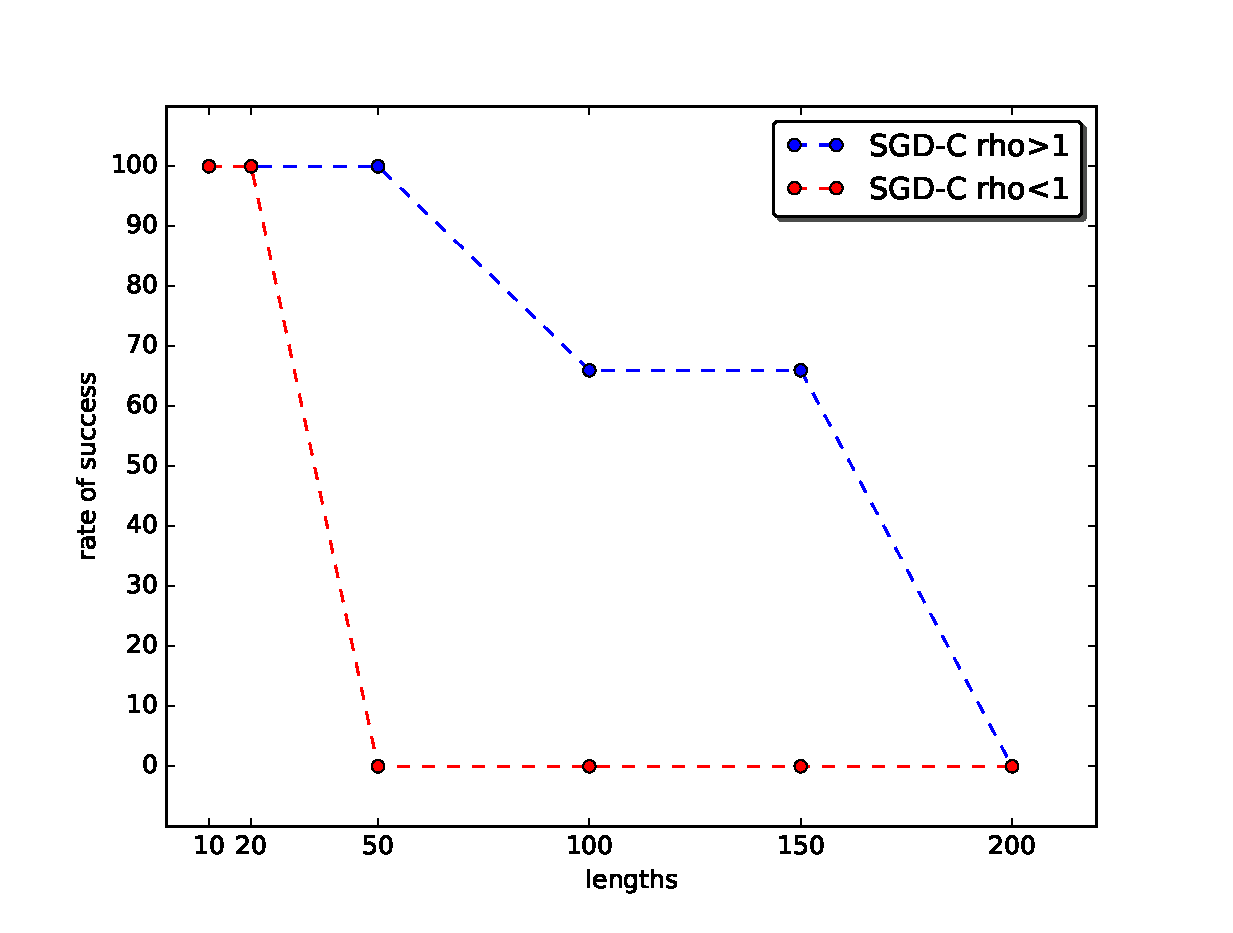
\includegraphics[width= 0.8\textwidth]{temporal_rates.eps}
		\caption{Rate of success for the temporal order task.}
		\label{fig:temporal_rates}
	\end{figure}
\end{frame}


\begin{frame}{A different descent direction}
	Combine the temporal gradients to obtain a descent direction which does not suffer from the vanishing gradient problem.
\begin{itemize}
	\item Normalize the temporal gradients:
	\begin{equation}
	s_t(\vec{x}) = \frac{\nabla L_{|t}(\vec{x})}{\norm{\nabla L_{|t}(\vec{x})}}.
	\end{equation}
	
	\item Combine the normalized gradients in a convex way:
	\begin{equation}
	s(\vec{x}) = \sum_{t=1}^T \beta_t \cdot s_t(\vec{x}).
	\end{equation}
	
	with $\sum_{t=1}^T\beta_t=1, \beta_t>0$ (randomly picked at each iteration).
	\item Introduce the gradient norm:
	\begin{equation}
	d(\vec{x}) = - \norm{\nabla L (\vec{x})}\frac{s(\vec{x})}{\norm{s(\vec{x})}}.
	\end{equation}
\end{itemize}
\end{frame}

\begin{frame}{}
	\begin{center}
		\scalebox{0.65}{
			\begin{minipage}{0.8\linewidth}
\begin{algorithm}[H]
	\KwData{\\
		\Indp
		$D=\{\pair{\vec{x}^{(i)}}{\vec{y}^{(i)}}\}$: training set\\
		$m$: size of each mini-batch\\
		$\mu$: constant learning rate\\
		$\tau$: gradient clipping threshold \\
		$\rho$: initial spectral radius \\
		$\psi$ threshold for the direction norm
	}
	
	
	$\mat{W_{rec}}, \mat{W_{in}, \mat{W_{out}}} \sim \mathcal{N}(0, \sigma^2)$\\
	$\vec{b}_{out}, \vec{b}_{rec} \gets 0$\\
	$r \gets \mbox{spectral\_radius}(\mat{W_{rec}})$\\
	$\mat{W_{rec}}\gets \frac{\rho}{r} \cdot \mat{W_{rec}}$\\
	$\theta_0 = [\mat{W_{rec}}, \mat{W_{in}}, \mat{W_{out}},\vec{b}_{out}, \vec{b}_{rec}]$
	
	
	\BlankLine
	\While{stop criterion}{
		
		$I$ $\gets$ sample $m$ training example $\in D$  \\
		$\{\nabla_\theta L_{|t}\}_{t=1}^{T} \gets \mbox{compute\_temporal\_gradients}(\theta_k, I)$\\
		$\vec{d}_k \gets \mbox{simplex\_combination}(\{\nabla_\theta L_{|t}\})$\\
		
		\If{$\norm{\nabla_{\theta}L(\theta_k)}_2 > \psi$}
		{$\vec{d}_k \gets \nabla_{\theta}L(\theta_k)$ \\
			\label{algo:line:condition}
		}
		
		$\alpha_k = 
		\begin{cases}
		\mu  \quad &\mbox{if} \norm{\vec{d}_k}_2 \leq \tau\\
		\frac{\mu \cdot \tau}{\norm{\vec{d}_k}_2} \quad & \mbox{otherwise}
		\end{cases}$\\
		
		$\theta_{k+1} \gets \theta_k + \alpha_k \vec{d}_k$\\
		$k\gets k+1$
	}
	\KwRet{$\theta_k$}
	\caption{RNN training}
	\label{algo:complete_solution}
\end{algorithm}
\end{minipage}%
}
\end{center}

\end{frame}

\begin{frame}{Effect of the simplex direction}
	
	\begin{figure}
		\centering
		\vspace{-2em}
	     \subfloat[][ Loss for the addition task during training.]{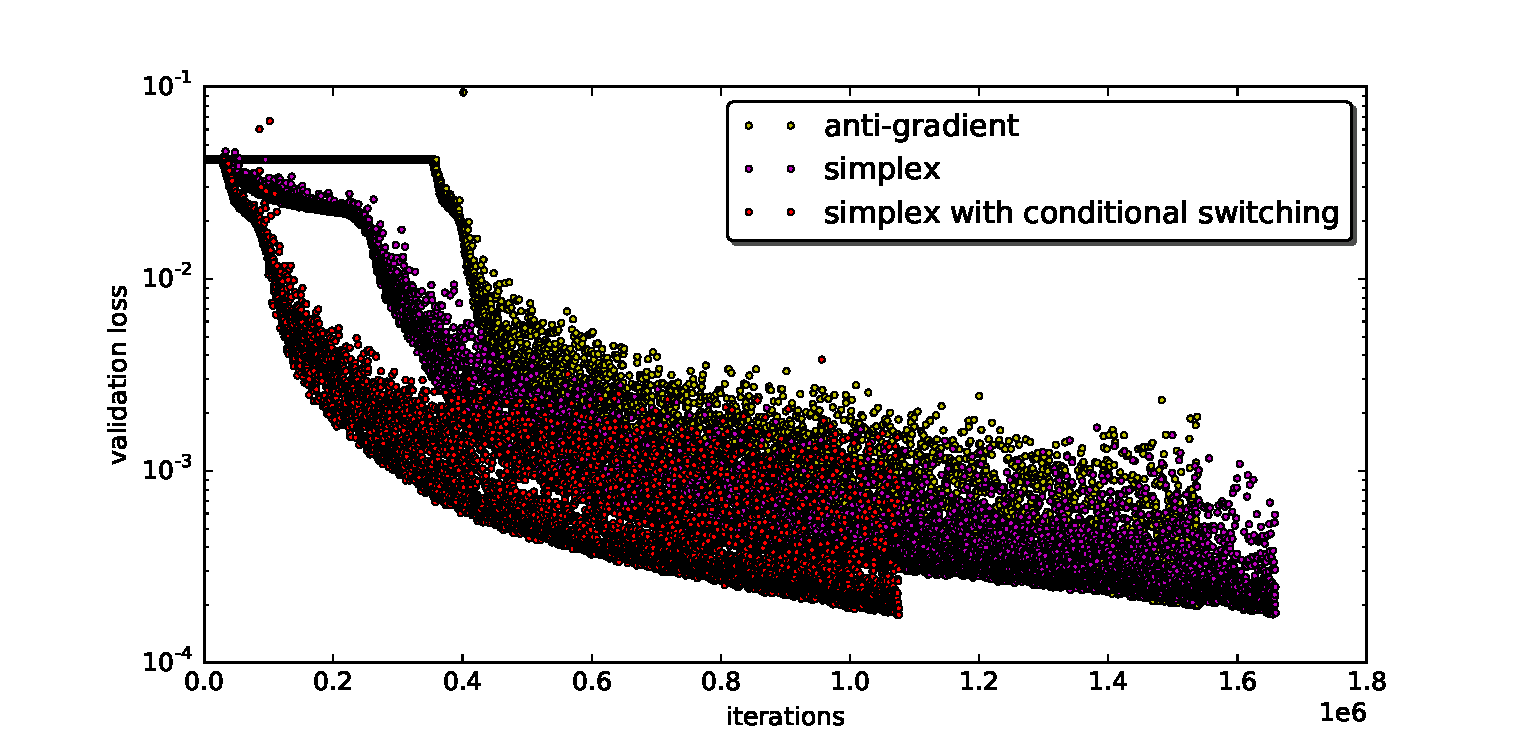
\includegraphics[width= 1\textwidth]{compare_simplex_add_new.eps}\label{fig:compare_add_13}}\\
	     \vspace{0em}
	     \subfloat[][Average number of iterations to converge.]{\raisebox{0em}{\resizebox{0.9\columnwidth}{!}{
	     		{\renewcommand{\arraystretch}{1.3}
	     			\setlength{\tabcolsep}{5pt}
	     		\begin{tabular}[b]{C{3cm} | C{3cm} C{5cm}}
	     		& anti-gradient & simplex with conditional switching \\
	     		\hline
	     		addition & 1807466 & \textbf{1630666} \\
	     		temporal order & 	2164800 & \textbf{1010000}\\
	     	\end{tabular}}}
	     }
	    }
%		\caption{Comparison between SGD using as descent direction the anti-gradient, the simplex direction and the simplex direction with conditional switching.}
		\label{fig:1}
	\end{figure}
	
%	\begin{figure}[h]
%		\begin{subfigure}{1.\textwidth}
%			\centering
%			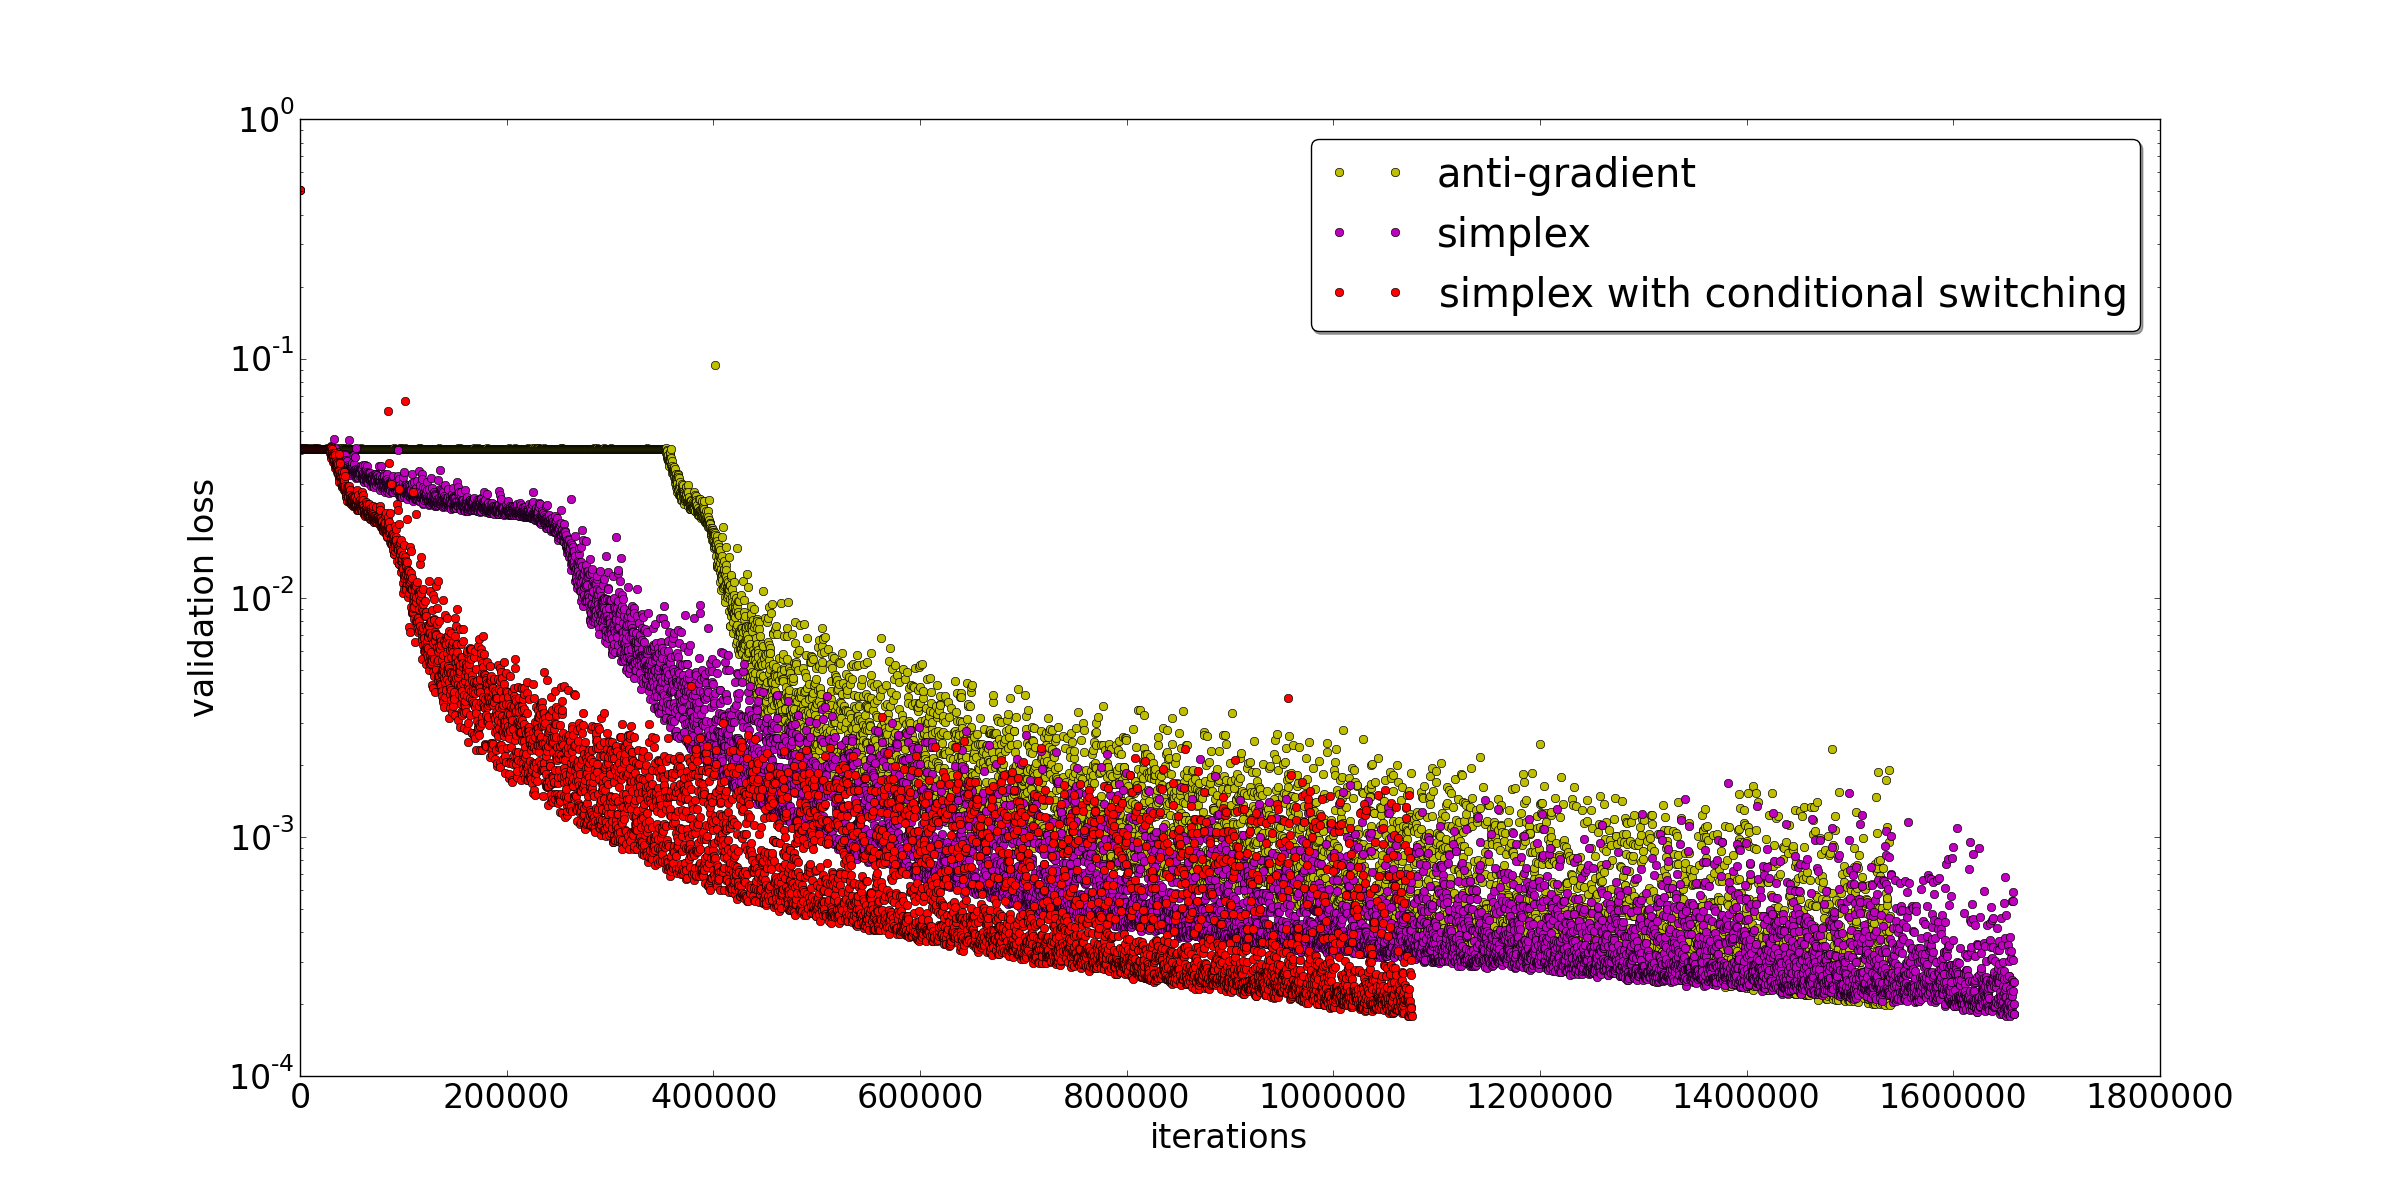
\includegraphics[width= 1\textwidth]{compare_add_simplex_13.png}
%			\caption{First run}
%			\label{fig:a:comparisong_add_simplex}
%		\end{subfigure}\\
%		\begin{subfigure}{1.\textwidth}
%			\centering
%			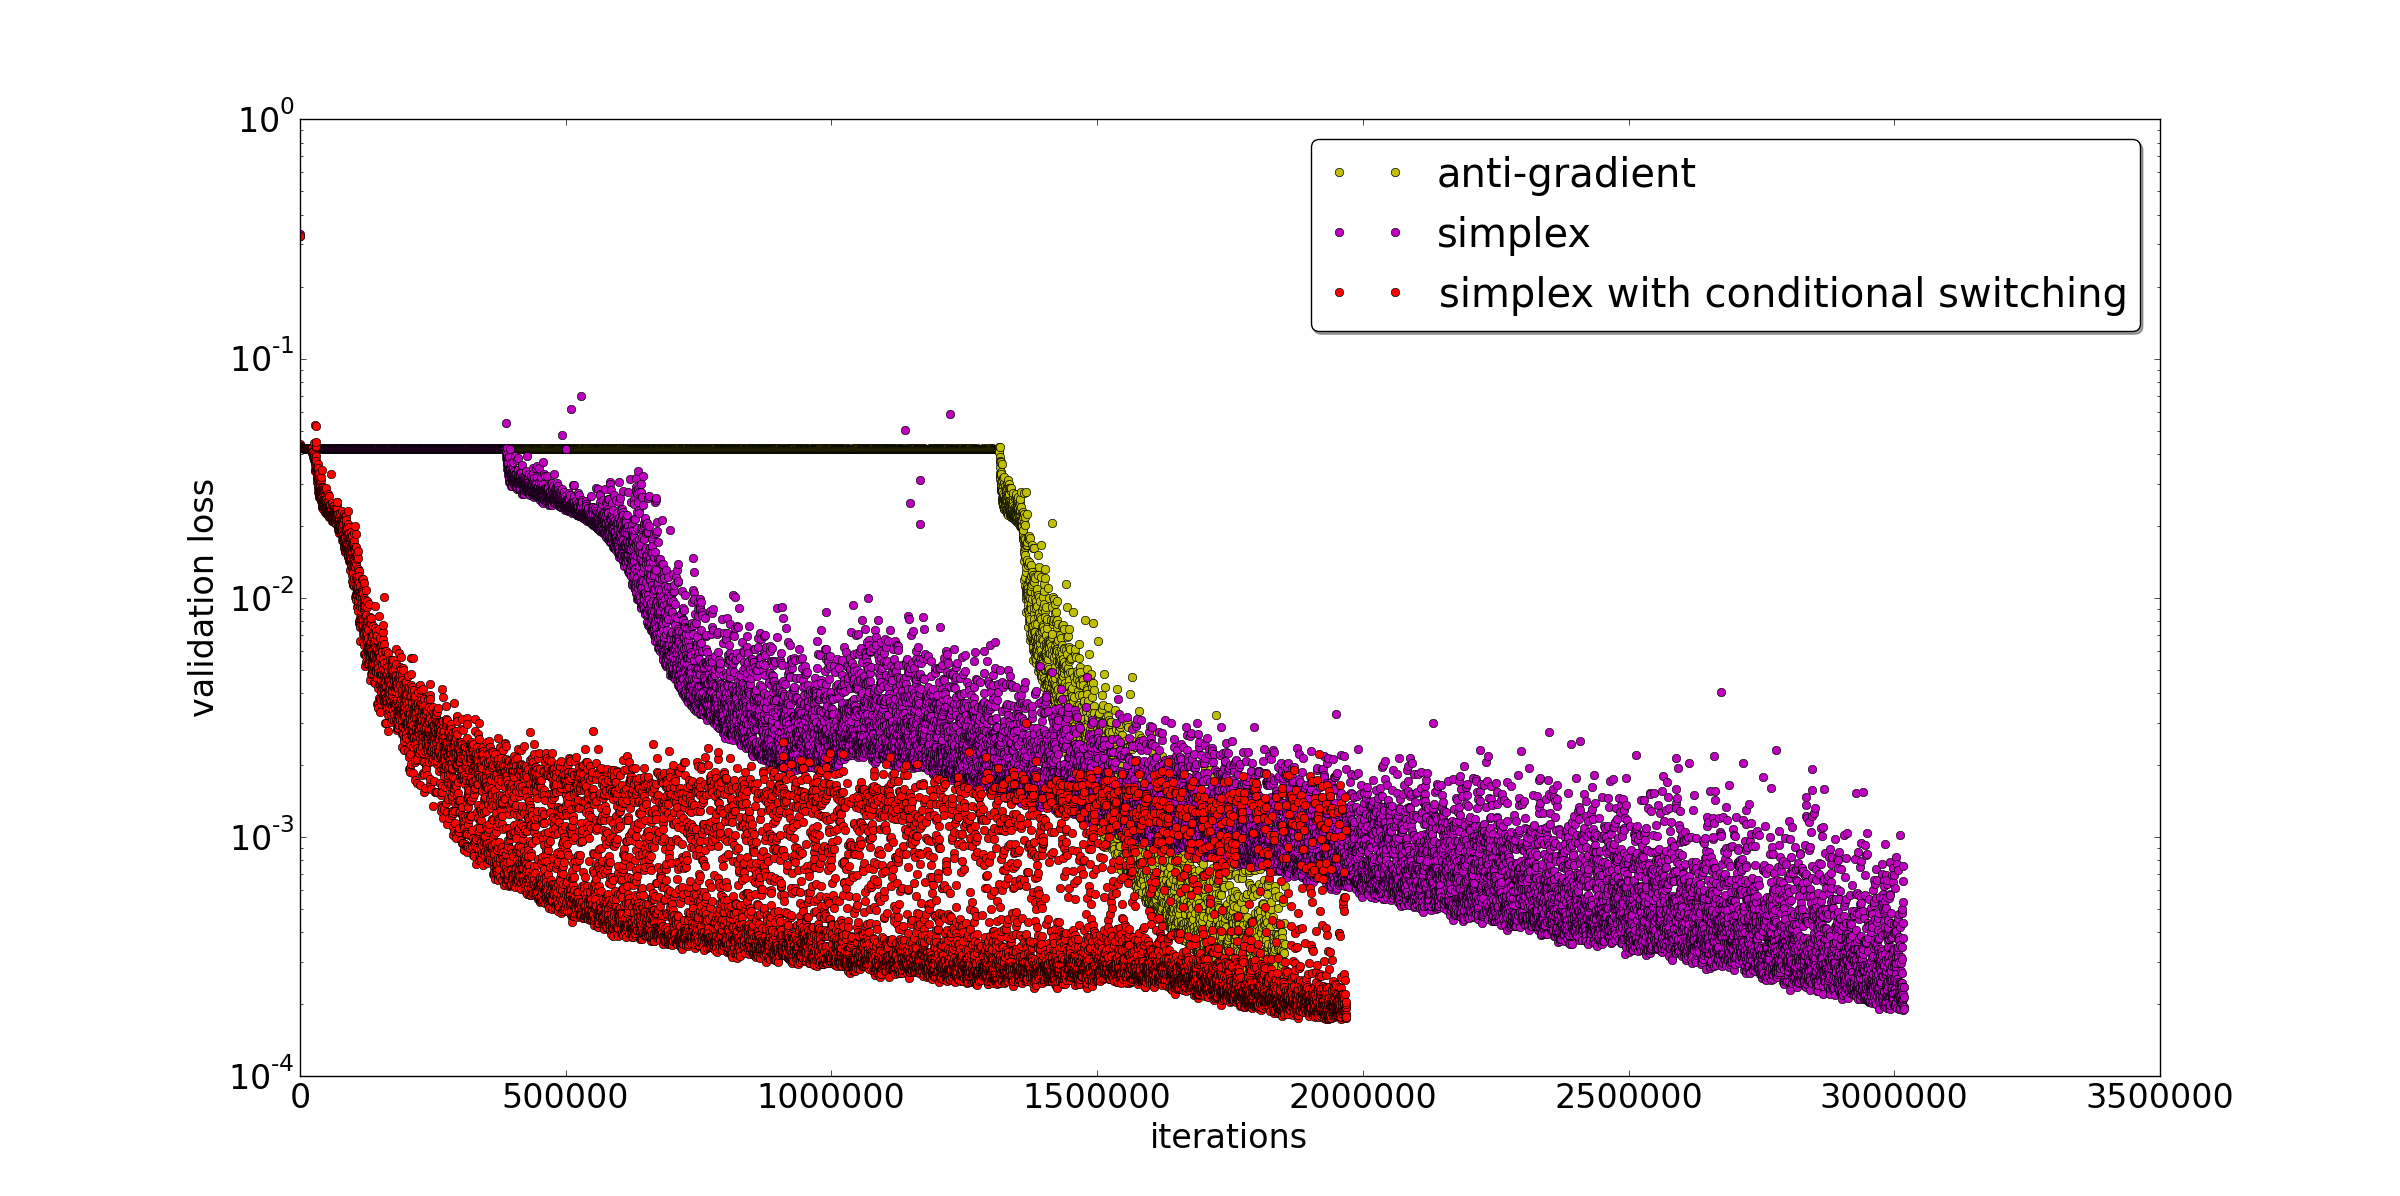
\includegraphics[width= 1\textwidth]{compare_add_simplex_14.png}
%			\caption{Second run}
%			\label{fig:b:comparisong_add_simplex}
%		\end{subfigure}\\
%		\begin{subfigure}{1.\textwidth}
%			\centering
%			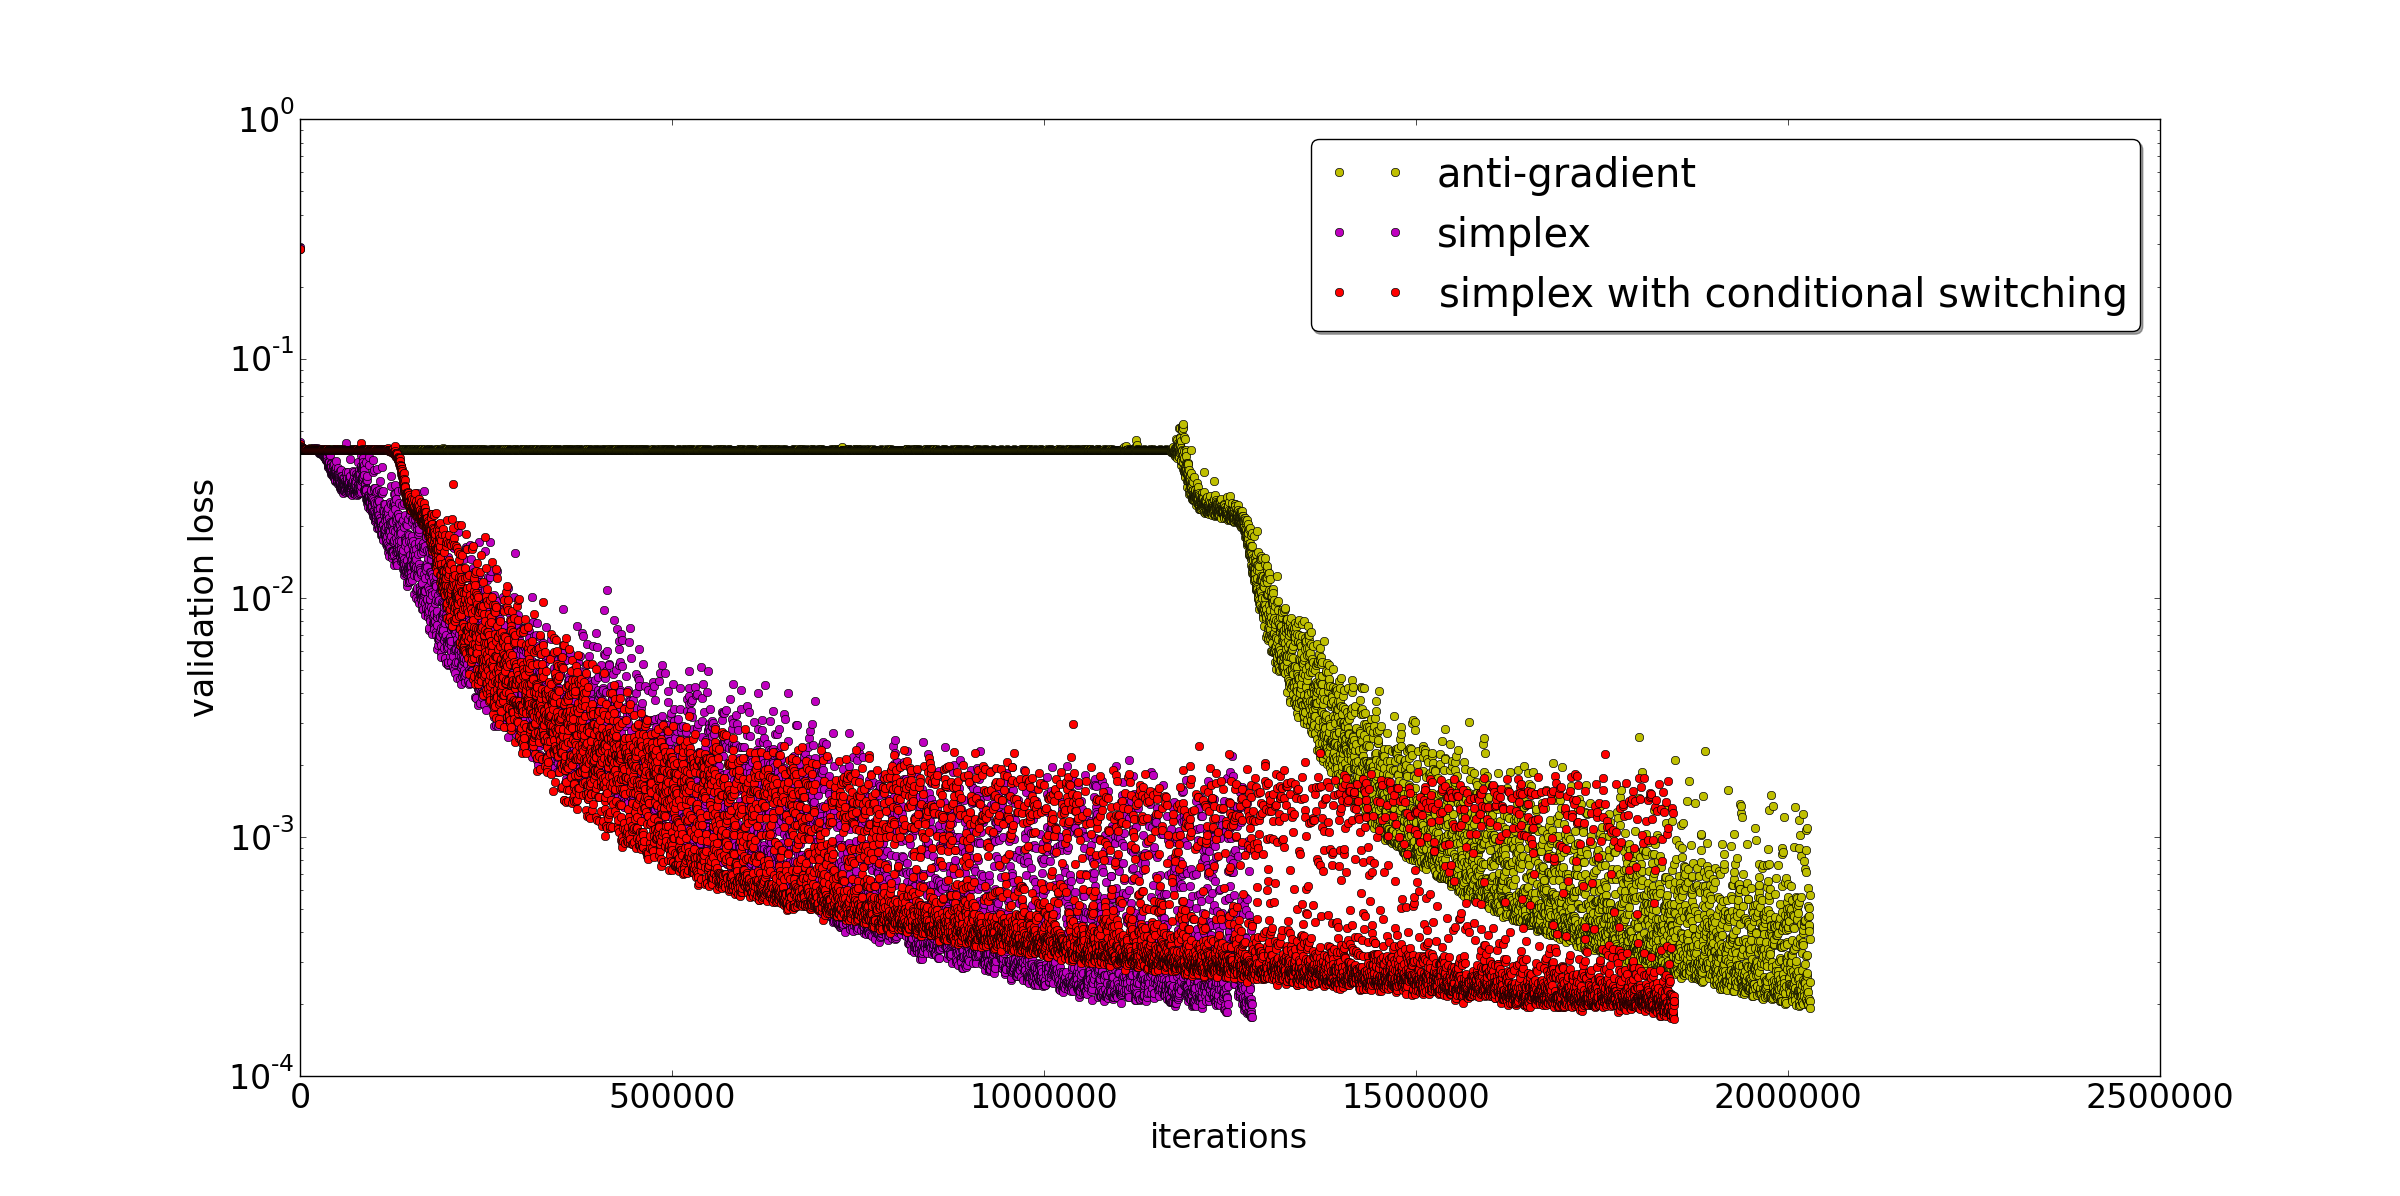
\includegraphics[width= 1\textwidth]{compare_add_simplex_15.png}
%			\caption{Third run}
%			\label{fig:c:comparisong_add_simplex}
%		\end{subfigure}%
%		\caption{Comparison between SGD using as descent direction the anti-gradient (in yellow, start decreasing always for last), the simplex direction (in purple, which is the second that start decreasing) and the simplex direction with conditional switching (in red, start decreasing always for first) for the addition task (T=100). In y axis the loss (mean squared error) in logarithmic scale.}
%		\label{fig:comparisong_add_simplex}
%	\end{figure}
\end{frame}

\section{A real case: Lupus disease prediction}

%\begin{table}
%	\begin{tabular}{ C{1.5cm} | C{0.7cm} C{2cm} C{1.5cm} C{1cm} C{1cm} C{1cm} C{2cm} C{2cm} | C{2cm} }
%		& age & MyasteniaGravis & arthritis & c3level & c4level & hematological & skinrash & sledai2kInferred & SDI \\
%		\hline
%		Visit 0 & 44.23 & 0 & 1 & 119 & 9 & 0 & 0 & 12.0 & 0 \\
%		Visit 1 & 44.63 & 0 & 0 & 96  & 7 & 0 & 0 & 2 & 0 \\
%		Visit 2 & 44.77 & 0 & 1 & 85.42 & 6 & 0 & 0 & 2 & 0 \\
%		Visit 3 & 44.98 & 0 & 1 & 76 & 6 & 0 & 0 & 2 & 0 \\
%		Visit 4:& 45.58 & 0 & 0 & 76 & 6 & 0 & 0 & 1 \\
%	\end{tabular}
%\end{table}

\begin{frame}{Lupus disease prediction}

	The \textbf{goal} is to predict whether a patience will develop the lupus disease in the near future given its medical history.
	\vspace{2em}\\
	Dataset:
	\begin{itemize}
		\item Gathered by the ``Lupus Clinic'', Reumatologia, Università Sapienza, Rome.
		\item Patients have a different number of visits.
		\item Visits are not equally spaced over time.
		\item Small dataset ($\sim100$ negatives, $40$ positives).
	\end{itemize}

\end{frame}

\begin{frame}{An example of a record of a patience}
\begin{table}[H]
	\centering
	\begin{tabular}{ C{2.5cm} | C{1cm} C{1cm} C{1cm} C{1cm} C{1cm}}
		& Visit 0 & Visit 1 & Visit 2 & Visit 3 & Visit 4 \\
		\hline
		age & 44.23 & 44.63 & 44.77 & 44.98 & 45.58 \\
		MyasteniaGravis & 0 & 0 & 0 & 0 & 0 \\
		arthritis & 1 & 0 & 1 & 1 & 0 \\
		c3level & 119 & 96 & 85.42 & 76 & 76 \\
		c4level & 9 & 7 & 6 & 6 & 6 \\
		hematological & 0 & 0 & 6 & 6 & 6 \\
		skinrash & 0 & 0 & 0 & 0 & 0 \\
		sledai2kInferred & 12 & 2 & 2 & 2 & 0 \\
		\dots & \dots & \dots & \dots & \dots & \dots \\
		\hline
		SDI & 0 & 0 & 0 & 0 & \textbf{1}\\
	\end{tabular}
\end{table}	
\end{frame}


\begin{frame}{Numerical results for the lupus disease prediction}

\begin{figure}
	\centering
		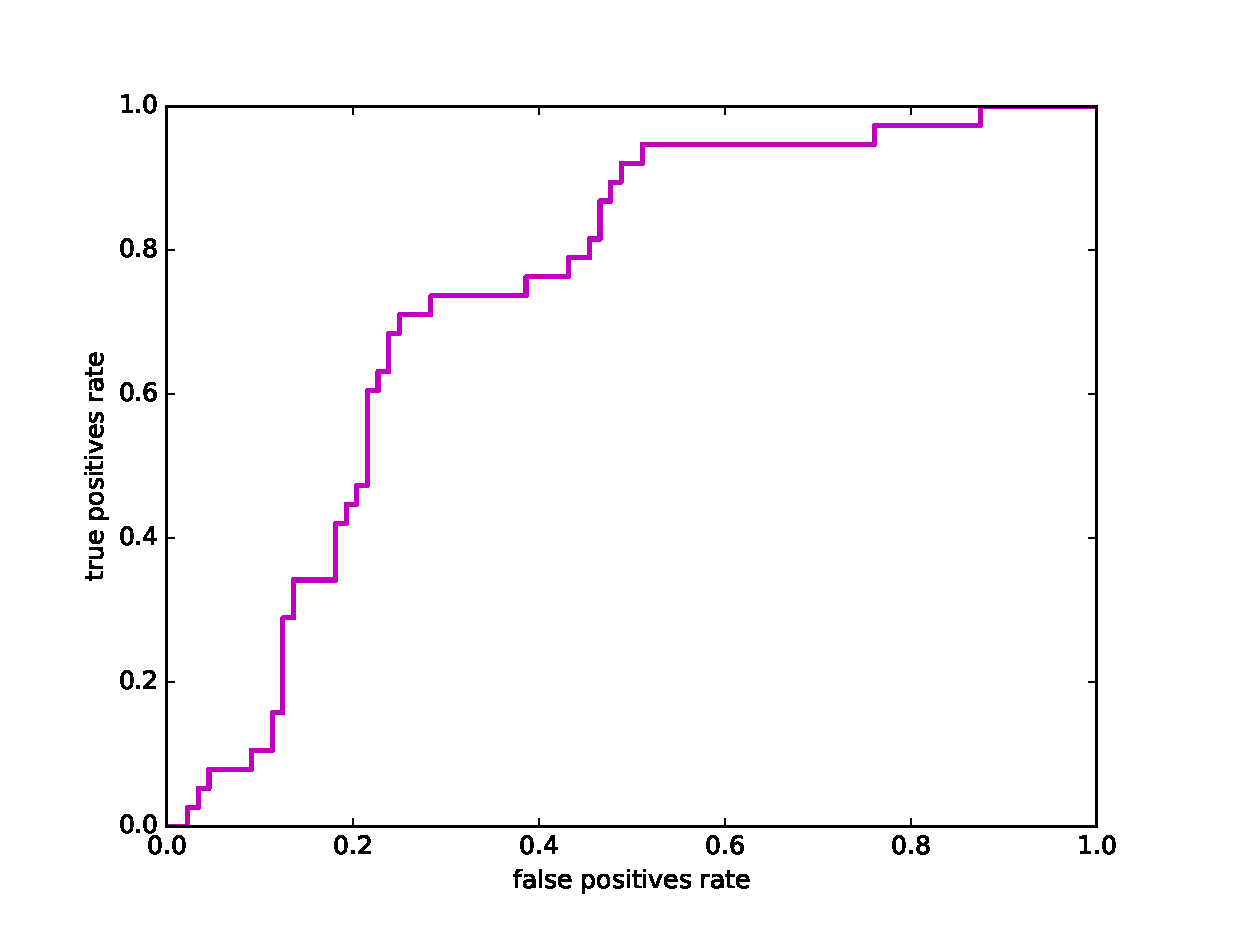
\includegraphics[width= 0.6\textwidth]{plot_roc_lupus_roc_.eps}
		%			\caption{roc curve for models of Line 5 of Table \ref{table:exp_res}.}
		\caption{ROC curve. AUC score is 0.74}
		\label{fig:lupus_roc}
\end{figure}

\begin{itemize}
	\item Results considered promising by medical experts.
	\item Improvable when more data will be available.
\end{itemize}

\end{frame}


 


\section{}
\begin{frame}[allowframebreaks]{References}
	\bibliographystyle{ieee}
	\bibliography{biblio}
\end{frame}

\end{document} 
